\documentclass[compress,11 pt,t]{beamer}
\usetheme[
	bullet=circle,		% Other option: square
	bigpagenumber,		% circled page number on lower right
	topline=true,		% colored bar at the top of the frame 
	]{Zurich}
%\useoutertheme[subsection=false]{miniframes}  
\usepackage[utf8]{inputenc} % Required for inputting international characters
\usepackage{multicol}
%\usepackage{media9}
\usepackage{multimedia}
\usefonttheme{professionalfonts}
\usepackage{arydshln}
\usepackage{amsmath}
\usepackage{amssymb}
\usepackage{subfigure}

%-----------------------------------------------------------------------------
% BEAMER TEMPLATE
\setbeamertemplate{section in toc}[sections numbered]
\setbeamerfont{subsection in toc}{size=\small}
\usepackage{etoolbox}
\makeatletter
\patchcmd{\slideentry}{\advance\beamer@xpos by1\relax}{}{}{}
\def\beamer@subsectionentry#1#2#3#4#5{\advance\beamer@xpos by1\relax}%
\makeatother

\def\algreen#1#2{{\only<#1>{\textcolor{tangocolordarkchameleon}{#2}}}}


%-----------------------------------------------------------------------------
% DOCUMENT PROPERTIES

\author[\textsc{Oriol Colomés Gené}]{\emph{author:}\\
\textsc{Oriol Colomés Gené}\\[0.2cm]
\emph{supervisor:}\\
\textsc{Santiago Badia}}
\title[Large scale FE solvers for LES of incomprssible turbulent flows]{Large scale Finite Element solvers for the large eddy simulation of incompressible turbulent flows}
\institute{Departament d'Enginyeria Civil i Ambiental}
\titlegraphic{
\includegraphics[width=0.5\textwidth]{../../sources/Figures/Cover/logo_escola_pantone_201_C}}
\date{March 31 2016}
%\titlegraphic{
\includegraphics[width=0.7\texwidth]{../../sources/Figures/Cover/logo_escola_pantone_201_C.png}}

%-----------------------------------------------------------------------------
%----------------------------------------------------------------------------------------
%	DEFINE CUSTOM SYMBOL COMMANDS
%----------------------------------------------------------------------------------------

% Bold
\def\u{{\bf u}}
\def\x{{\bf x}}
\def\r{{\bf r}}
\def\e{{\bf e}}
\def\a{{\bf a}}
\def\v{{\bf v}}
\def\w{{\bf w}}
\def\f{{\bf f}}
\def\n{{\bf n}}
\def\t{{\bf t}}
\def\k{{\bf k}}
\def\R{{\bf R}}
\def\F{{\bf F}}
\def\U{{\bf U}}
\def\P{{\bf P}}
\def\X{{\bf X}}
\def\H{\bf{H}}
\def\Lbf{{\bf L}}
\def\Hbf{{\bf H}}
\def\Tbf{{\bf T}}
\def\Cbf{{\bf C}}
\def\Rbf{{\bf R}}
\def\boldI{\mathbf{I}}

% Bold symbols
\def\XI{{\boldsymbol{\Xi}}}
\def\kppa{\boldsymbol{\kappa}}
\def\etaa{\boldsymbol{\eta}}
\def\xii{\boldsymbol{\xi}}
\def\KA{\boldsymbol{\Kappa}}
\def\ETA{\boldsymbol{\Upsilon}}
\def\boldsigma{\boldsymbol{\sigma}}
\def\boldomega{\boldsymbol{\omega}}
\def\boldzeta{\boldsymbol{\zeta}}

%Caligraphic
\def\Dcal{\mathcal{D}}
\def\Ccal{\mathcal{C}}

% BB
\def\M{\mathbb{M}}
\def\K{\mathbb{K}}
\def\C{\mathbb{C}}
\def\G{\mathbb{G}}
\def\D{\mathbb{D}}
\def\L{\mathbb{L}}
\def\A{\mathbb{A}}
\def\B{\mathbb{B}}
\def\I{\mathbb{I}}
\def\Sb{\mathbb{S}}
\def\Kt{\tilde{\mathbb{K}}}
\def\Bt{\tilde{\mathbb{B}}}
\def\Mt{\tilde{\mathbb{M}}}
\def\St{\tilde{\mathbb{S}}}
\def\At{\tilde{\mathbb{A}}}
\def\T{\mathbb{T}}
\def\Rbb{\mathbb{R}}

% Other
\def\half{\frac{1}{2}}
\def\Eq#1{(\ref{eq-#1})}
\def\Lem#1{\ref{lem-#1}}
\def\Fig#1{Figure \ref{fig-#1}}
\def\Chap#1{Chapter \ref{chap-#1}}
\def\Sec#1{Section \ref{sec-#1}}
\def\cl{ \nonumber \\}
\def\el{\nonumber}
\def\jumpl{\lbrack\!\lbrack}
\def\jumpr{\rbrack\!\rbrack}
\def\jump#1{\jumpl #1 \jumpr}
\def\jumpt#1{\underline{\jump{#1}}}
\def\mean#1{\{\! \!\{ #1\}\! \!\}}
\def\meanpv#1{\{ #1\}}
\def\meanhar#1{\langle#1\rangle}
\def\Qq{ \Omega \times (0,t^*)}

% New commands
\newtheorem{remark}{Remark}[section]
\newtheorem{proposition}{Proposition}[section]
\newcommand{\tickYes}{\checkmark}
\newcommand{\tickNo}{\hspace{1pt}\ding{55}}
\definecolor{tableShade}{HTML}{F1F5FA}



\begin{document}

%=========================================================================================
% TITLE
% ----------------------------------------------------------------------------
\addtocounter{framenumber}{-1}
\frame{\titlepage}
% ----------------------------------------------------------------------------
\addtocounter{framenumber}{-1}
\frame{\vfill\tableofcontents[subsectionstyle=hide,subsubsectionstyle=hide]\vfill}

%=========================================================================================
% 1.MOTIVATION
% ----------------------------------------------------------------------------
\section{Motivation}
\addtocounter{framenumber}{-1}
\frame{\vfill
	\tableofcontents[currentsection,
		 			  subsubsectionstyle=hide,						  sectionstyle=show/shaded, 
					  subsectionstyle=show/hide]
					  \vfill
}
\begin{frame}
\frametitle{Motivation}
\vfill
{\bf Thesis motivation }\\
\begin{itemize}
\item<2-> Turbulence is a very challenging problem:
\begin{itemize}
\item Many industrial applications
\item Understanding the phenomena (physics)
\end{itemize}
\item<3-> Computational Fluid Dynamics (CFD) to simulate such flows
\item<4-> Take advantage of increasing computational capacity (High-performance Computing (HPC))
\item<5-> In a Finite Element (FE) framework
\end{itemize}
\vfill
\end{frame}
%=========================================================================================
\begin{frame}
\frametitle{Objective}
\vfill
{\bf Thesis goal }\\
Highly scalable Finite Element (FE) framework for Large Eddy Simulations (LES) of incompressible turbulent flows\\
\vspace{0.5cm}
\onslide<2->{{\bf How to get there?}
\begin{enumerate}
\onslide<3->{\item \alert<3>{Variational MultiScale} (VMS) methods as LES models}
\onslide<4->{\item Time integration schemes with \alert<4>{velocity-pressure segregation}}
\onslide<5->{\item Highly scalable algorithms based on \alert<5>{Domain Decomposition (DD) and block preconditioners}}
\end{enumerate}}
\vfill
\end{frame}
%=========================================================================================
\begin{frame}
\frametitle{Objective}
\vfill
\textbf{Step by step...}
\begin{itemize}
\onslide<1->{\alert<6>{\item Residual-based VMS as LES models}}
\onslide<2->{\item Mixed FE formulations as LES models}
\onslide<3->{\item High-order time integration schemes}
\onslide<4->{\item Velocity-pressure segregation}
\onslide<5->{\item Scalable solvers}
\end{itemize}
\vfill
\end{frame}

%=========================================================================================
% 2.RESIDUAL-BASED VMS
% ----------------------------------------------------------------------------
\section{Residual-based VMS}
\addtocounter{framenumber}{-1}
\frame{
\begin{minipage}[\textheight]{0.5\textwidth}
\vfill
\tableofcontents[currentsection,
				subsubsectionstyle=hide,
				sectionstyle=show/shaded, 
				subsectionstyle=show/show/hide]
\vfill
\end{minipage}
\begin{minipage}[\textheight]{0.4\textwidth}
	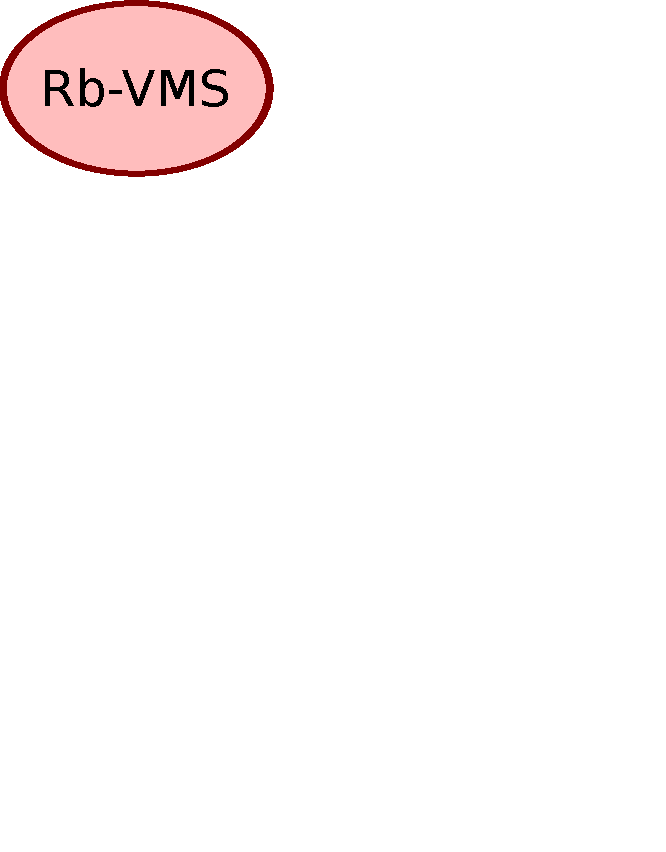
\includegraphics[width=1.1\textwidth]{Figures/index_1}
\end{minipage}
}
\begin{frame}
\frametitle{Implicit LES}
\vfill
\textbf{ILES}: only numerical dissipation (for stabilization) acts as turbulent model
\begin{overprint}
\onslide<1>
\begin{itemize}
\item Not based on filtering of the Navier-Stokes equations
\item Rely on numerical artifacts, no modification at the continuous level
\end{itemize}
\end{overprint}
\vfill
\end{frame}

%=========================================================================================
% 2.1.FORMULATION
% ----------------------------------------------------------------------------
\subsection{Formulation}
%----------------------------------------------------------------------------------------
\begin{frame}[t]
\frametitle{Incomp. Navier Stokes equations}
Find $ \mathbf{u}$ and $p$ defined in $\Omega$
\begin{align*}
\partial _{t}\mathbf{u}+ {\color<4>{red} \mathbf{u}\cdot \mathbf{\nabla u} }+\mathbf{
\nabla }p-\nu \nabla ^{2}\mathbf{u}& =\mathbf{f} \\
\mathbf{\nabla }\cdot \mathbf{u}& =0
\end{align*}
with appropriate boundary conditions on $ \Gamma$.\vskip 0.3cm
\only<2->{
The weak problem is: $\forall \mathbf{v}\in \mathcal{V}_0$ and  $\forall q\in \mathcal{Q}_0$, 
find $ \mathbf{u} \in \mathcal{V}$ and $ p \in \mathcal{Q}$ such that 
\begin{align*}
  \left( \mathbf{v},\partial_{t}\mathbf{u}\right)_{\Omega }
+ \left( \mathbf{\nabla v}, \nu \mathbf{\nabla u}\right)_{\Omega }  
%+ {\color<4>{red} \langle \mathbf{v},\mathbf{a}\cdot \mathbf{\nabla u}\rangle _{\Omega }} 
+ {\color<4>{red} b\left(\mathbf{u},\mathbf{u}, \mathbf{v}\right)} % \\
- \left( \mathbf{\nabla }\cdot \mathbf{v},p\right) _{\Omega } 
& = 
\left\langle \mathbf{v},\mathbf{f} \right\rangle _{\Omega } 
\\
\left(q, \mathbf{\nabla } \cdot \mathbf{u}\right)_{\Omega } 
& = 0
\end{align*}}
\only<3->{where
\begin{equation*}
{\color<4>{red} 
b\left(\mathbf{a},\mathbf{u}, \mathbf{v}\right) = {\color<1-3>{white} \frac{1}{2}}\langle \mathbf{v},\mathbf{a}\cdot \mathbf{\nabla u}\rangle_{\Omega }
{\color<1-3>{white} - \frac{1}{2} \langle \mathbf{a}\cdot\mathbf{\nabla}\mathbf{v}, \mathbf{u}\rangle_{\Omega }
+ \frac{1}{2} \langle \mathbf{v},\mathbf{n} \cdot \mathbf{a}  \mathbf{u} \rangle_{\Gamma }}}
\end{equation*}
}
\end{frame}
%----------------------------------------------------------------------------------------
\begin{frame}[t]
\frametitle{VMS decomposition {\small (Hughes 1995)}}
A decomposition of spaces $\mathcal{V}$ and $\mathcal{Q}$ given by 
\begin{equation*}
\mathcal{V}=\mathcal{V}_{h}\oplus \widetilde{\mathcal{V}},\quad
\mathcal{Q}=\mathcal{Q}_{h}\oplus \widetilde{\mathcal{Q}}
\end{equation*}
\only<2->{is applied to the function and test spaces
\begin{align*}
\mathbf{u} = \mathbf{u}_{h} +\widetilde{\mathbf{u}}, \quad p = p_h + \widetilde{p} \\
\mathbf{v} = \mathbf{v}_{h} +\widetilde{\mathbf{v}}, \quad q = q_h + \widetilde{q}
\end{align*}}
\only<3->{We keep all the (eight) contributions from the splitting of the convective
term 
\begin{equation*}
  { \mathbf{u}} \cdot \mathbf{\nabla u}
= { \mathbf{u}_{h}\cdot \mathbf{\nabla u}_{h} }
+ { \color<3->{red} \widetilde{\mathbf{u}}\cdot \mathbf{\nabla u}_{h} }
+ { \mathbf{u}_{h}\cdot \mathbf{\nabla }\widetilde{\mathbf{u}} }
+ { \color<3->{red} \widetilde{\mathbf{u}}\cdot \mathbf{\nabla }\widetilde{\mathbf{u}} }
\end{equation*}
}
\only<4->{and all the (four) contributions from the temporal term 
\begin{equation*}
\partial _{t}\mathbf{u}=\partial _{t}\mathbf{u}_{h} + { \color<4->{red} \partial _{t}\widetilde{\mathbf{u}}}
\end{equation*}
}
\end{frame}
%----------------------------------------------------------------------------------------
\begin{frame}[t]
\frametitle{Semidiscrete problem}
\begin{block}{FEM equations}
\begin{overlayarea}{\textwidth}{2.0cm}
\vspace{-0.8cm}
\begin{align*}
% FEM EQUATIONS
\only<1>{B\left(\left(\mathbf{u}_h,p_h\right);\left(\widetilde{\mathbf{u}},\widetilde{p}\right);\left(\mathbf{v}_h,q_h\right)\right)=L\left(\mathbf{v}_h,q_h\right)}
\only<2->{\left( \mathbf{v}_{h},\partial _{t}\mathbf{u}_{h}\right) _{\Omega }
%+\langle \mathbf{v}_{h},\mathbf{a}\cdot \mathbf{\nabla u}_{h}\rangle _{\Omega}
+ b\left(\mathbf{a},\mathbf{u}_h, \mathbf{v}_h\right)
+\left( \mathbf{\nabla v}_{h},\nu \mathbf{\nabla u}_{h}\right) _{\Omega} &
-\left( \mathbf{\nabla }\cdot \mathbf{v}_{h},p_{h}\right) _{\Omega }
\\[0.05in]
%
+\left( \mathbf{v}_{h},\partial _{t}\widetilde{\mathbf{u}}\right) _{\Omega}
+\left( \mathcal{L}^{\ast }\mathbf{v}_{h},\widetilde{\mathbf{u}}\right)_{\Omega^h}
-\left( \mathbf{\nabla }\cdot \mathbf{v}_{h},\widetilde{p}\right) _{\Omega^h} &
=\left\langle \mathbf{v}_{h},\mathbf{f}\right\rangle_{\Omega }
\\[0.1in]
%
\left( q_{h},\mathbf{\nabla }\cdot \mathbf{u}_{h}\right) _{\Omega }
-\left( \mathbf{\nabla }q_{h},\widetilde{\mathbf{u}}\right) _{\Omega^h} & =0}
\end{align*}
\end{overlayarea}
\end{block}
\begin{block}{SGS equations}
\vspace{-0.4cm}
\begin{align*}
% SGS EQUATIONS
\only<1>{B\left(\left(\widetilde{\mathbf{u}},\widetilde{p}\right);\left(\mathbf{u}_h,p_h\right);\left(\widetilde{\mathbf{v}},\widetilde{q}\right)\right)=L\left(\widetilde{\mathbf{v}},\widetilde{q}\right)}
%\only<1-4>{\left( \widetilde{\mathbf{v}},\partial_{t} \widetilde{\mathbf{u}} \right)_{\Omega }}
%\only<1-2>{\color<2>{red}  + \left( \widetilde{\mathbf{v}},\mathcal{L}\widetilde{\mathbf{u}}\right )_{\Omega^h}}
%\only<3-4>{\color<3>{red}  + \tau _{m}^{-1} \left( \widetilde{\mathbf{v}},\widetilde{\mathbf{u}} \right)_{\Omega^h}}
%\only<1-2>{\color<2>{blue} + \left( \widetilde{\mathbf{v}},\mathbf{\nabla }\widetilde{p}\right)_{\Omega^h} }
%%\only<1-4>{\color{white}\tau _{m}^{-1}} % This is needed to avoid a vertical blinking 
\only<2-> {{\color<5>{red} \partial_{t}\widetilde{\mathbf{u}}} + {\color<2>{red}\tau_{m}^{-1}} \widetilde{\mathbf{u}}}
&
\only<2-> { = {\color<4>{red}\mathcal{P}} {\color<3>{red}\mathbf{R}_{m} }}
\only<1>{\\[0.05in]}
%
%\only<1->{{ \color{white}\tau_{c}^{-1} }}
%\only<1-4>{ \color<4>{red}
%+\left( \widetilde{\mathbf{v}},\partial _{t}\mathbf{u}_{h}\right)_{\Omega}
%+\left( \widetilde{\mathbf{v}},\mathcal{L}\mathbf{u}_{h}\right)_{\Omega^h}
%+\left( \widetilde{\mathbf{v}},\mathbf{\nabla }p_{h}\right)_{\Omega^h}
%& = 
%\color<4>{red} \left\langle \widetilde{\mathbf{v}},\mathbf{f}\right\rangle _{\Omega} }
%%
\\[0.1in]
%%
%%\only<1->{{ \color{white}\tau_{c}^{-1} }}
%\only<1-2>{{\color<2>{blue} \left(( \widetilde{q},\mathbf{\nabla} \cdot \widetilde{\mathbf{u}}\right)_{\Omega }}}
%\only<3-4>{{\color<3>{blue} \tau_{c}^{-1} \left( \widetilde{q},\widetilde{p}\right) _{\Omega^h }}}
%\only<1-4>{ + {\color<4>{blue} \left( \widetilde{q},\mathbf{\nabla}\cdot \mathbf{u}_{h}\right)_{\Omega } }} 
%\only<1-4>{& = 0}
\only<2->{ {\color<2>{blue} \tau _{c}^{-1}} \widetilde{p} & = {\color<4>{blue}\mathcal{P}} {\color<3>{blue}R_{c}}}
\end{align*}
\end{block}
%\end{overlayarea}
\vspace{-0.2cm}
\begin{overlayarea}{\textwidth}{3.0cm}
\only<1>{
\vspace*{-1.0cm}
\begin{equation*}
%\mathcal{L}=-\nu \nabla ^{2}+\mathbf{a}\cdot \mathbf{\nabla },\quad 
%\mathcal{L}^{\ast }=-\nu \nabla ^{2}-\mathbf{a}\cdot \mathbf{\nabla },\quad
%\mathbf{a=u}_{h}+\widetilde{\mathbf{u}}
\end{equation*}
}
\only<2>{
\begin{equation*}
{ \color<2>{red} \tau_{m}=\left( \frac{c_{1}\nu }{h^{2}}+\frac{c_{2}\left| \mathbf{a}\right| }{h}\right) ^{-1}},\quad
{ \color<2>{blue}\tau_{c}=\frac{h^{2}}{c_{1}\tau _{m}} }
\end{equation*}
}
\only<3>{
\begin{equation*}
{ \color<3>{red} \mathbf{R}_{m}} := \mathbf{f} - \partial_{t}\mathbf{u}_{h} - \mathcal{L} \mathbf{u}_{h} - \mathbf{\nabla }p_{h}, \quad
{ \color<3>{blue} R_{c}} := - \mathbf{\nabla }\cdot \mathbf{u}_{h}
\end{equation*}
}
\only<4->{
\begin{equation*}
\only<4>{{\color<4>{red} \mathcal{P} = I \quad \rm{(ASGS)}}, \quad \quad {\color<4>{blue} \mathcal{P} = P_h^{\perp}=I-P_h \quad \rm{(OSS)}} }
\only<5->{{\color<5>{magenta} \mathcal{P} = I \quad \rm{(ASGS)}, \quad \quad  \mathcal{P} = P_h^{\perp}=I-P_h \quad \rm{(OSS)} }}
\end{equation*}
}
\only<2,5>{
\vspace{-0.2cm}
\begin{equation*}
{\color<5>{blue} \mathbf{a=u}_{h}+\widetilde{\mathbf{u}} }
\end{equation*}
}
\end{overlayarea}
%
%\begin{overlayarea}{\textwidth}{1.5cm}
%%\only<3->{
%\begin{equation*}
%{\color<6>{blue} \mathbf{a=u}_{h}+\widetilde{\mathbf{u}}} 
%{\color<1-2>{white}, \quad \tau_{m}=\left(( \frac{c_{1}\nu }{h^{2}}+\frac{c_{2}\left| \mathbf{a}\right| }{h}\right) ^{-1},\quad
%\tau_{c}=\frac{h^{2}}{c_{1}\tau _{m}} }
%\end{equation*}
%%}
%\end{overlayarea}
\end{frame}


%=========================================================================================
% 2.2.ENERGY STATEMENTS
% ----------------------------------------------------------------------------
%\subsection{Energy statements}
%\begin{frame}[t]
\frametitle{Energy statements}
\begin{overlayarea}{\textwidth}{0.25\textheight}
\textbf{FE counterpart:}
\vspace*{-0.3cm}
\only<1>{
\begin{align*}
&B\left(\left(\mathbf{u}_h,p_h\right);\left(\widetilde{\mathbf{u}},\widetilde{p}\right);\left(\mathbf{u}_h,p_h\right)\right)=L\left(\mathbf{u}_h,p_h\right)
\end{align*}}
\only<2->{
\begin{align*}
&\alert<3>{\frac{1}{2}d_t\|\u_h\|^2}+\alert<4>{\nu\|\nabla\u_h\|^2}+\alert<5>{b(\a,\u_h,\u_h)}\\
&\alert<7>{+\left( \partial _{t}\widetilde{\u},\u_{h}\right)
+\left( \mathcal{L}^{\ast }_a(\u_{h},p_h),\widetilde{\u}\right)
-\left( \mathbf{\nabla }\cdot \u_{h},\widetilde{p}\right)}
=\alert<8>{\left\langle \mathbf{f},\u_{h}\right\rangle}
\end{align*}}
\end{overlayarea}
\begin{overlayarea}{\textwidth}{0.25\textheight}
\textbf{SGS counterpart:}
\vspace*{-0.3cm}
\only<1>{
\begin{align*}
&B\left(\left(\widetilde{\mathbf{u}},\widetilde{p}\right);\left(\mathbf{u}_h,p_h\right);\left(\widetilde{\mathbf{u}},\widetilde{p}\right)\right)=L\left(\widetilde{\mathbf{u}},\widetilde{p}\right)
\end{align*}}
\only<2->{
\begin{align*}
&\alert<3>{\frac{1}{2}d_t\|\widetilde{\u}\|^2}\alert<6>{+\tau_m^{-1}\|\widetilde{\u}\|^2+\tau_c^{-1}\|\widetilde{p}\|^2}\\
&\alert<7>{+\left( \mathcal{P}(\partial _{t}\u_{h}),\widetilde{\u}\right)
+\left( \mathcal{P}(\mathcal{L}^{\ast }_a(\u_{h},p_h)),\widetilde{\u}\right)
-\left( \mathcal{P}(\mathbf{\nabla }\cdot \u_{h}),\widetilde{p}\right)}
=\alert<8>{\left\langle \mathcal{P}(\mathbf{f}),\widetilde{\u}\right\rangle}
\end{align*}}
\end{overlayarea}
\begin{overlayarea}{\textwidth}{0.5\textheight}
\textbf{TOTAL:}
\only<9>{\alert<9>{\textbf{ Static subscales}}}
\only<10->{\alert<10->{\textbf{ Dynamic subscales}}}
\only<10>{\alert<10>{\textbf{- ASGS}}}
\only<11>{\alert<11>{\textbf{- OSS}}}
\only<1>{
\begin{align*}
&B\left(\left(\mathbf{u}_h,p_h\right);\left(\widetilde{\mathbf{u}},\widetilde{p}\right);\left(\mathbf{u}_h,p_h\right)\right)\\
+&B\left(\left(\widetilde{\mathbf{u}},\widetilde{p}\right);\left(\mathbf{u}_h,p_h\right);\left(\widetilde{\mathbf{u}},\widetilde{p}\right)\right)=L\left(\mathbf{u}_h,p_h\right)+L\left(\widetilde{\mathbf{u}},\widetilde{p}\right)
\end{align*}}
\only<3-8>{
\begin{align*}
&\alert<3>{\frac{1}{2}d_t\|\u_h\|^2+\frac{1}{2}d_t\|\widetilde{\u}\|^2}
\onslide<4-8>{
\alert<4>{+\nu\|\nabla\u_h\|^2}
\onslide<6-8>{
\alert<6>{+\tau_m^{-1}\|\widetilde{\u}\|^2+\tau_c^{-1}\|\widetilde{p}\|^2}\\
\onslide<7-8>{
&\alert<7>{+\left( \partial _{t}\widetilde{\u},\u_{h}\right)+\left( \mathcal{P}(\partial _{t}\u_{h}),\widetilde{\u}\right)
+\left( \mathcal{L}^{\ast }_a(\u_{h},p_h),\widetilde{\u}\right)+\left( \mathcal{P}(\mathcal{L}^{\ast }_a(\u_{h},p_h)),\widetilde{\u}\right)}\\
&\alert<7>{
-\left( \mathbf{\nabla }\cdot \u_{h},\widetilde{p}\right)
-\left( \mathcal{P}(\mathbf{\nabla }\cdot \u_{h}),\widetilde{p}\right)}
\onslide<8>{
=\alert<8>{\left\langle \mathbf{f},\u_{h}\right\rangle+\left\langle \mathcal{P}(\mathbf{f}),\widetilde{\u}\right\rangle}
}}}}
\end{align*}}
\only<9->{
\begin{align*}
&\only<9,11>{\frac{1}{2}d_t\|\u_h\|^2}
\only<10>{\frac{1}{2}d_t\|\u_h+\widetilde{\u}\|^2}
\onslide<11>{+\frac{1}{2}d_t\|\widetilde{\u}\|^2}
+\nu\|\nabla\u_h\|^2
+\tau_m^{-1}\|\widetilde{\u}\|^2+\tau_c^{-1}\|\widetilde{p}\|^2\\
&\only<9>{\onslide<11>{+\left( \partial _{t}\widetilde{\u},\u_{h}\right)}+\left( \mathcal{P}(\partial _{t}\u_{h}),\widetilde{\u}\right)
+\left( \mathcal{L}^{\ast }_a(\u_{h},p_h),\widetilde{\u}\right)+\left( \mathcal{P}(\mathcal{L}^{\ast }_a(\u_{h},p_h)),\widetilde{\u}\right)}
\only<10,11>{-2\left( \nu\Delta\u_h,\widetilde{\u}\right)}\\
&\onslide<9>{-\left( \mathbf{\nabla }\cdot \u_{h},\widetilde{p}\right)
-\left( \mathcal{P}(\mathbf{\nabla }\cdot \u_{h}),\widetilde{p}\right)}
=\left\langle \mathbf{f},\u_{h}\right\rangle
\only<9,11>{+\left\langle \mathcal{P}(\mathbf{f}),\widetilde{\u}\right\rangle}
\only<10>{+\left\langle \mathbf{f},\widetilde{\u}\right\rangle}
\end{align*}}
\end{overlayarea}

\end{frame}

%=========================================================================================
% 2.3.NUMERICAL EXPERIMENTS
% ----------------------------------------------------------------------------
\subsection{Numerical experiments}
\begin{frame}[t]
\frametitle{Numerical experiments}
\vfill
Three different turbulent benchmarks:
\begin{itemize}
\item Decaying of Homogeneous Isotropic Turbulence (DHIT)
\item Taylor-Green Vortex (TGV) flow
\item Turbulent Channel Flow (TCF)
\end{itemize}
\vfill
\end{frame}

%=========================================================================================
% 2.3.1.DHIT
% ----------------------------------------------------------------------------
\subsubsection{DHIT}
%----------------------------------------------------------------------------------------
\begin{frame}
  \frametitle{DHIT{\small Decay of Homogeneous Isotropic Turbulence}}
  \textbf{Problem setting:}
  \begin{itemize}
  \itemsep0cm
  \item Prescribed initial energy spectra corresponding to $Re_{\lambda}=952$.
  \item Setting defined in AGARD database (Mansour \& Wray 1993). 
  \item A (very simple) time step adaptation technique is used.
  \item Different mesh discretizations ($ Q_1/Q_1 $ and $ Q_2/Q_2 $).
  \end{itemize}
  \vspace{-0.1cm}
  \begin{figure}
      \centering	
      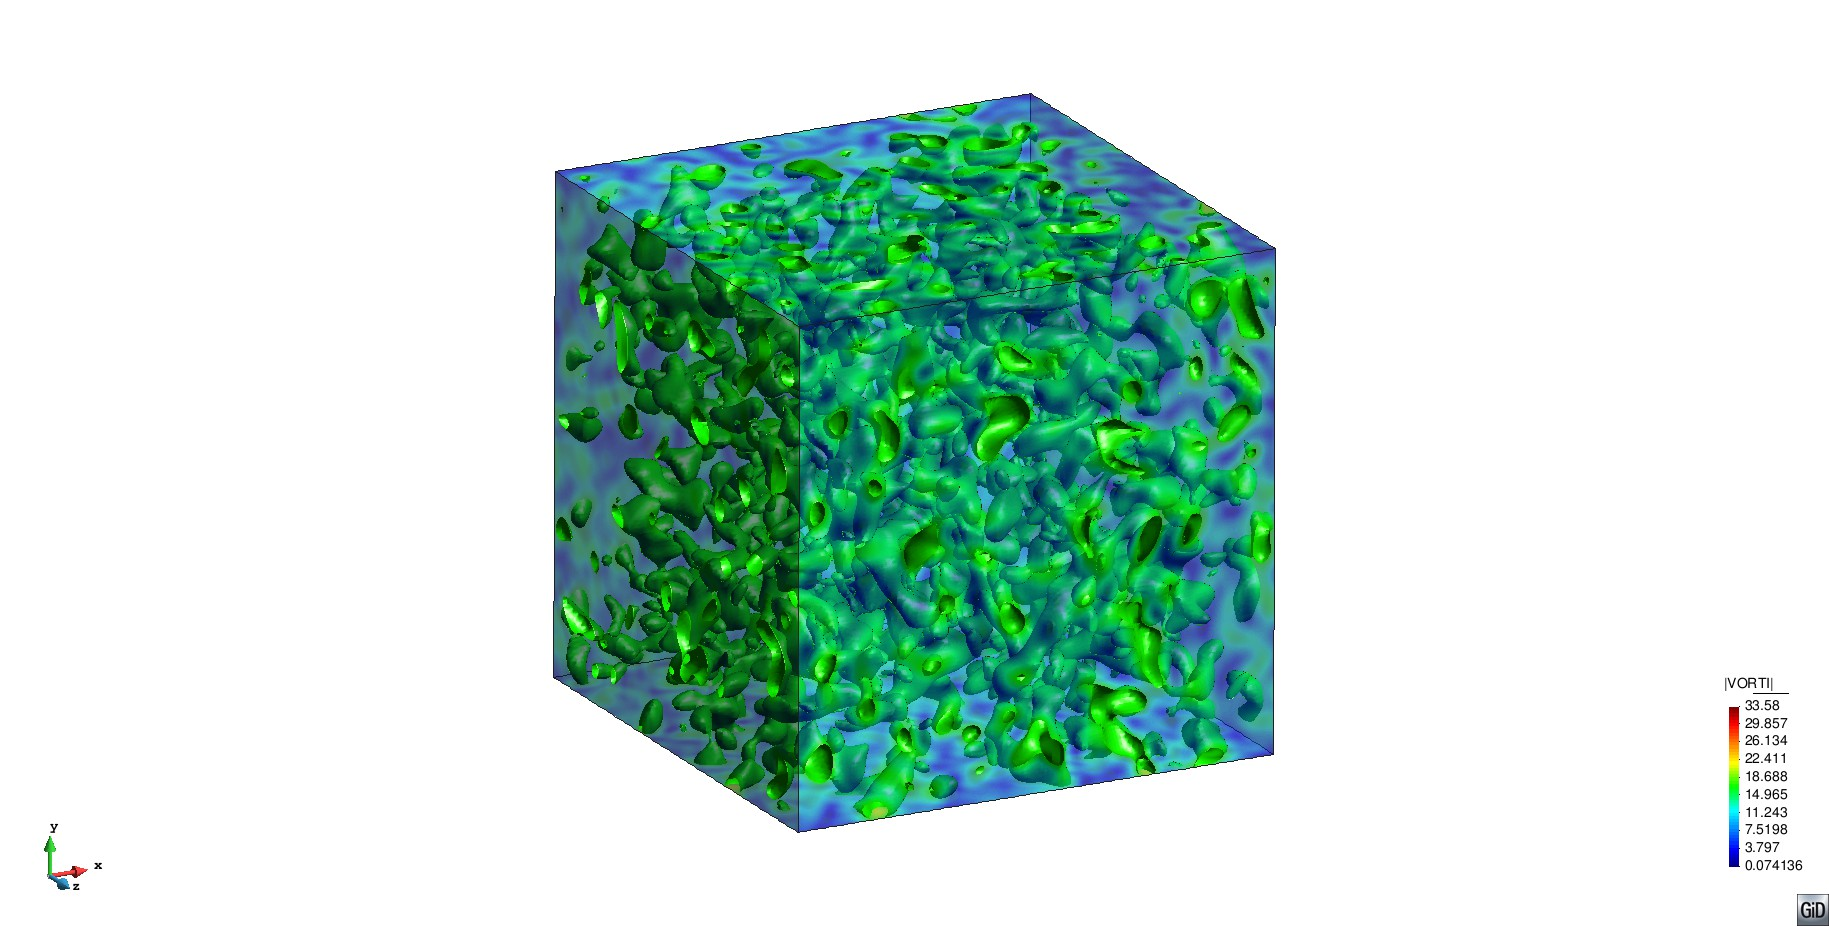
\includegraphics[clip=true,trim=19cm 2cm 19cm 3cm,width=0.45\textwidth]{Figures/iso_vorti_1.jpg}
  \end{figure}
\end{frame}
%----------------------------------------------------------------------------------------
\begin{frame}[t]
  \frametitle{DHIT{\small Decay of Homogeneous Isotropic Turbulence}}
  \textbf{Energy espectra (models):}
  \vspace*{-1.0cm}
  \begin{columns}
  \begin{column}{0.5\textwidth}
  \begin{figure}
    \centering	
    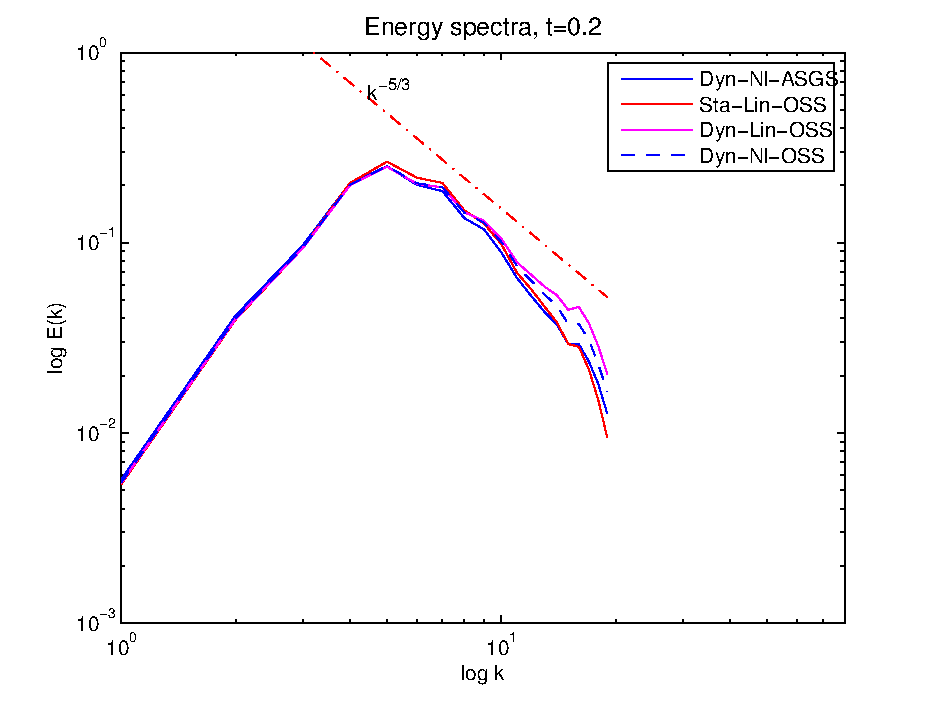
\includegraphics[width=1.1\textwidth]{Figures/spec_32_02_scaled}
    \vspace*{-0.8cm}
    \caption{$32^3-Q1$, $t=0.2s$}
  \end{figure}
  \end{column}
  \begin{column}{0.5\textwidth}
    \begin{figure}
    \centering	
    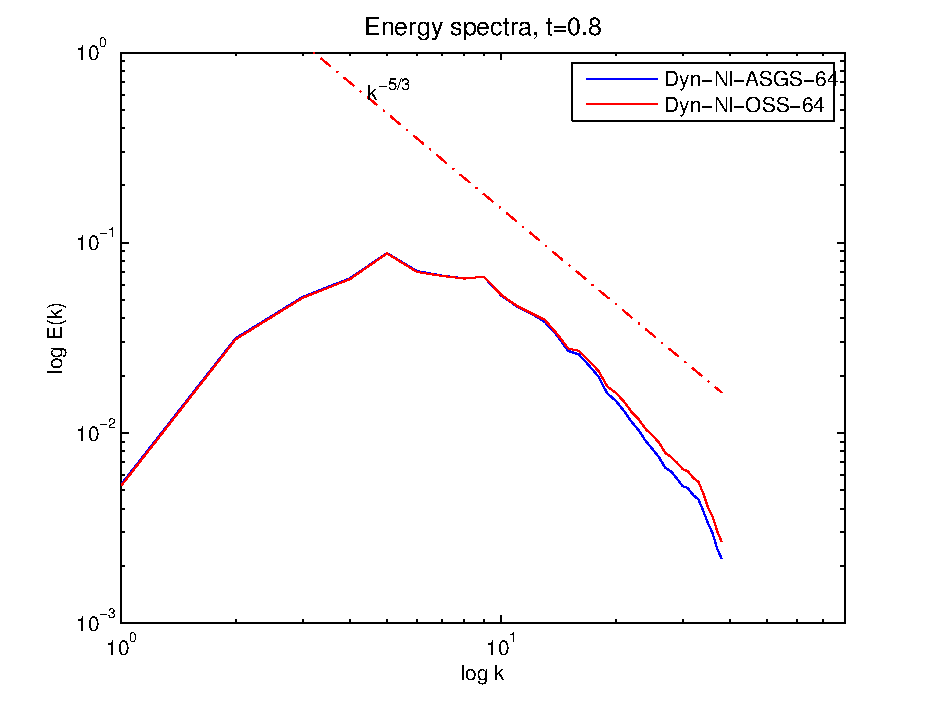
\includegraphics[width=1.1\textwidth]{Figures/spec_64_08}
    \vspace*{-0.8cm}
    \caption{$64^3-Q1$, $t=0.8s$}
  \end{figure}
  \end{column}
  \end{columns}
  \vspace*{-0.3cm}
  \begin{overlayarea}{\textwidth}{1.5cm}
  \only<2->{
  \begin{itemize}
  	\item \alert<2>{Small differences} between methods (physical sense).
  	\only<3->{\item Even \alert<3>{more similar when we refine} the mesh.}
  \end{itemize}}
  \end{overlayarea}
\end{frame}
%----------------------------------------------------------------------------------------
\begin{frame}
\frametitle{DHIT{\small Decay of Homogeneous Isotropic Turbulence}}
\textbf{Computational cost (models):}
 \vspace*{-1.0cm}
 \begin{columns}
 \begin{column}{0.5\textwidth}
 \begin{figure}
  \centering
  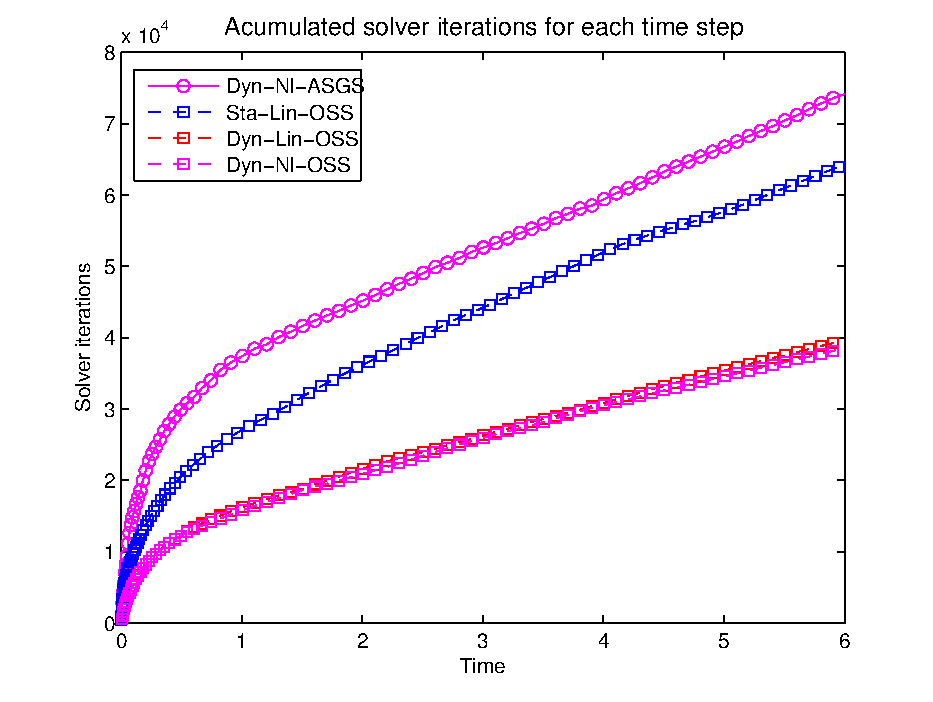
\includegraphics[width=1.1\textwidth]{Figures/Acsoliter_32_scaled_cnvgd}
      \vspace*{-0.8cm}
  \caption{$32^3-Q1$}
  \end{figure}
  \end{column}
  \begin{column}{0.5\textwidth}
   \begin{figure}
  \centering
  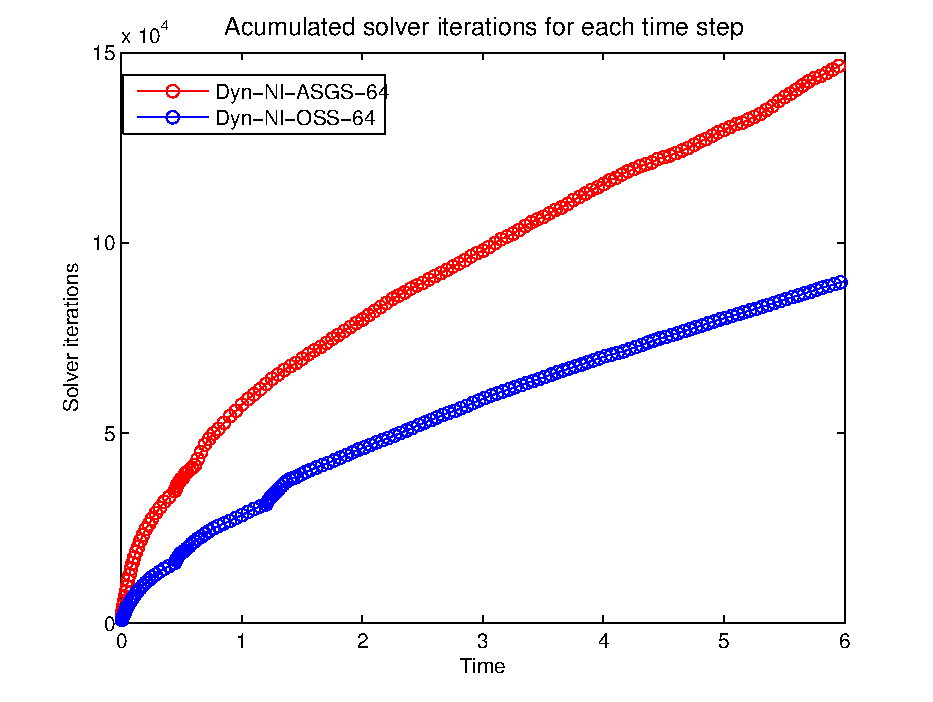
\includegraphics[width=1.1\textwidth]{Figures/Acsoliter_64}
      \vspace*{-0.8cm}
  \caption{$64^3-Q1$}
  \end{figure}
  \end{column}
  \end{columns}
  \begin{overlayarea}{\textwidth}{1.5cm}
  \vspace*{-0.3cm}
  \only<2->{
  \begin{itemize}
  	\item \alert<2>{Big differences} between methods (computational sense).
  	\only<3->{\item \alert<3>{Dynamic} versions of \alert<3>{OSS} method are \alert<3>{the most efficient}.}
  \end{itemize}}
  \end{overlayarea}
\end{frame}
%----------------------------------------------------------------------------------------
\begin{frame}[t]
  \frametitle{DHIT{\small Decay of Homogeneous Isotropic Turbulence}}
  \textbf{Energy espectra (refinement):}
  \begin{figure}
    \centering	
    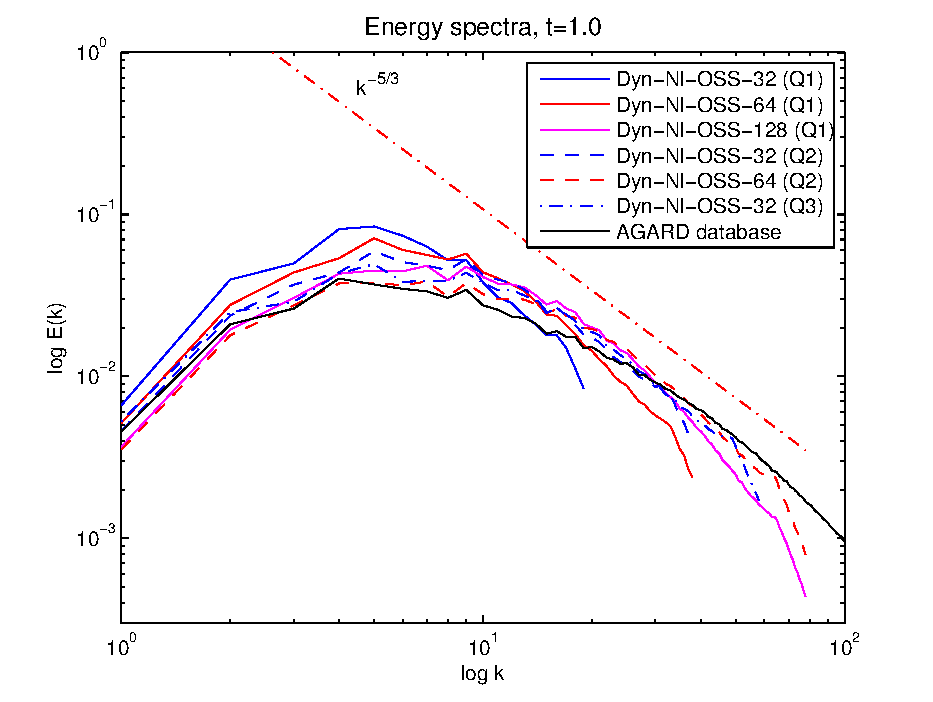
\includegraphics[width=0.7\textwidth]{Figures/spec_hp_1}
  \end{figure}
  \begin{overlayarea}{\textwidth}{1.5cm}
  \vspace*{-0.6cm}
  \begin{itemize}
  	\item Results become \alert<1->{closer to the DNS when we refine} the mesh.
  \end{itemize}
  \end{overlayarea}
\end{frame}

%=========================================================================================
% 2.3.2.TGV
% ----------------------------------------------------------------------------
\subsubsection{TGV}
%----------------------------------------------------------------------------------------
\begin{frame}
  \frametitle{TGV {\small Taylor-Green Vortex flow}}
  \only<1-2>{
  \textbf{Problem setting:}
  \begin{itemize}
    \itemsep-0.10cm
 	\item Prescribed initial condition
  	\item $Re=1600$
	\item Different mesh discretizations ($ Q_1/Q_1 $ and $ Q_2/Q_2 $)
  \end{itemize}
  \only<1>{
  	  \vspace*{-0.3cm}
	  \begin{figure}
	    \centering	
	    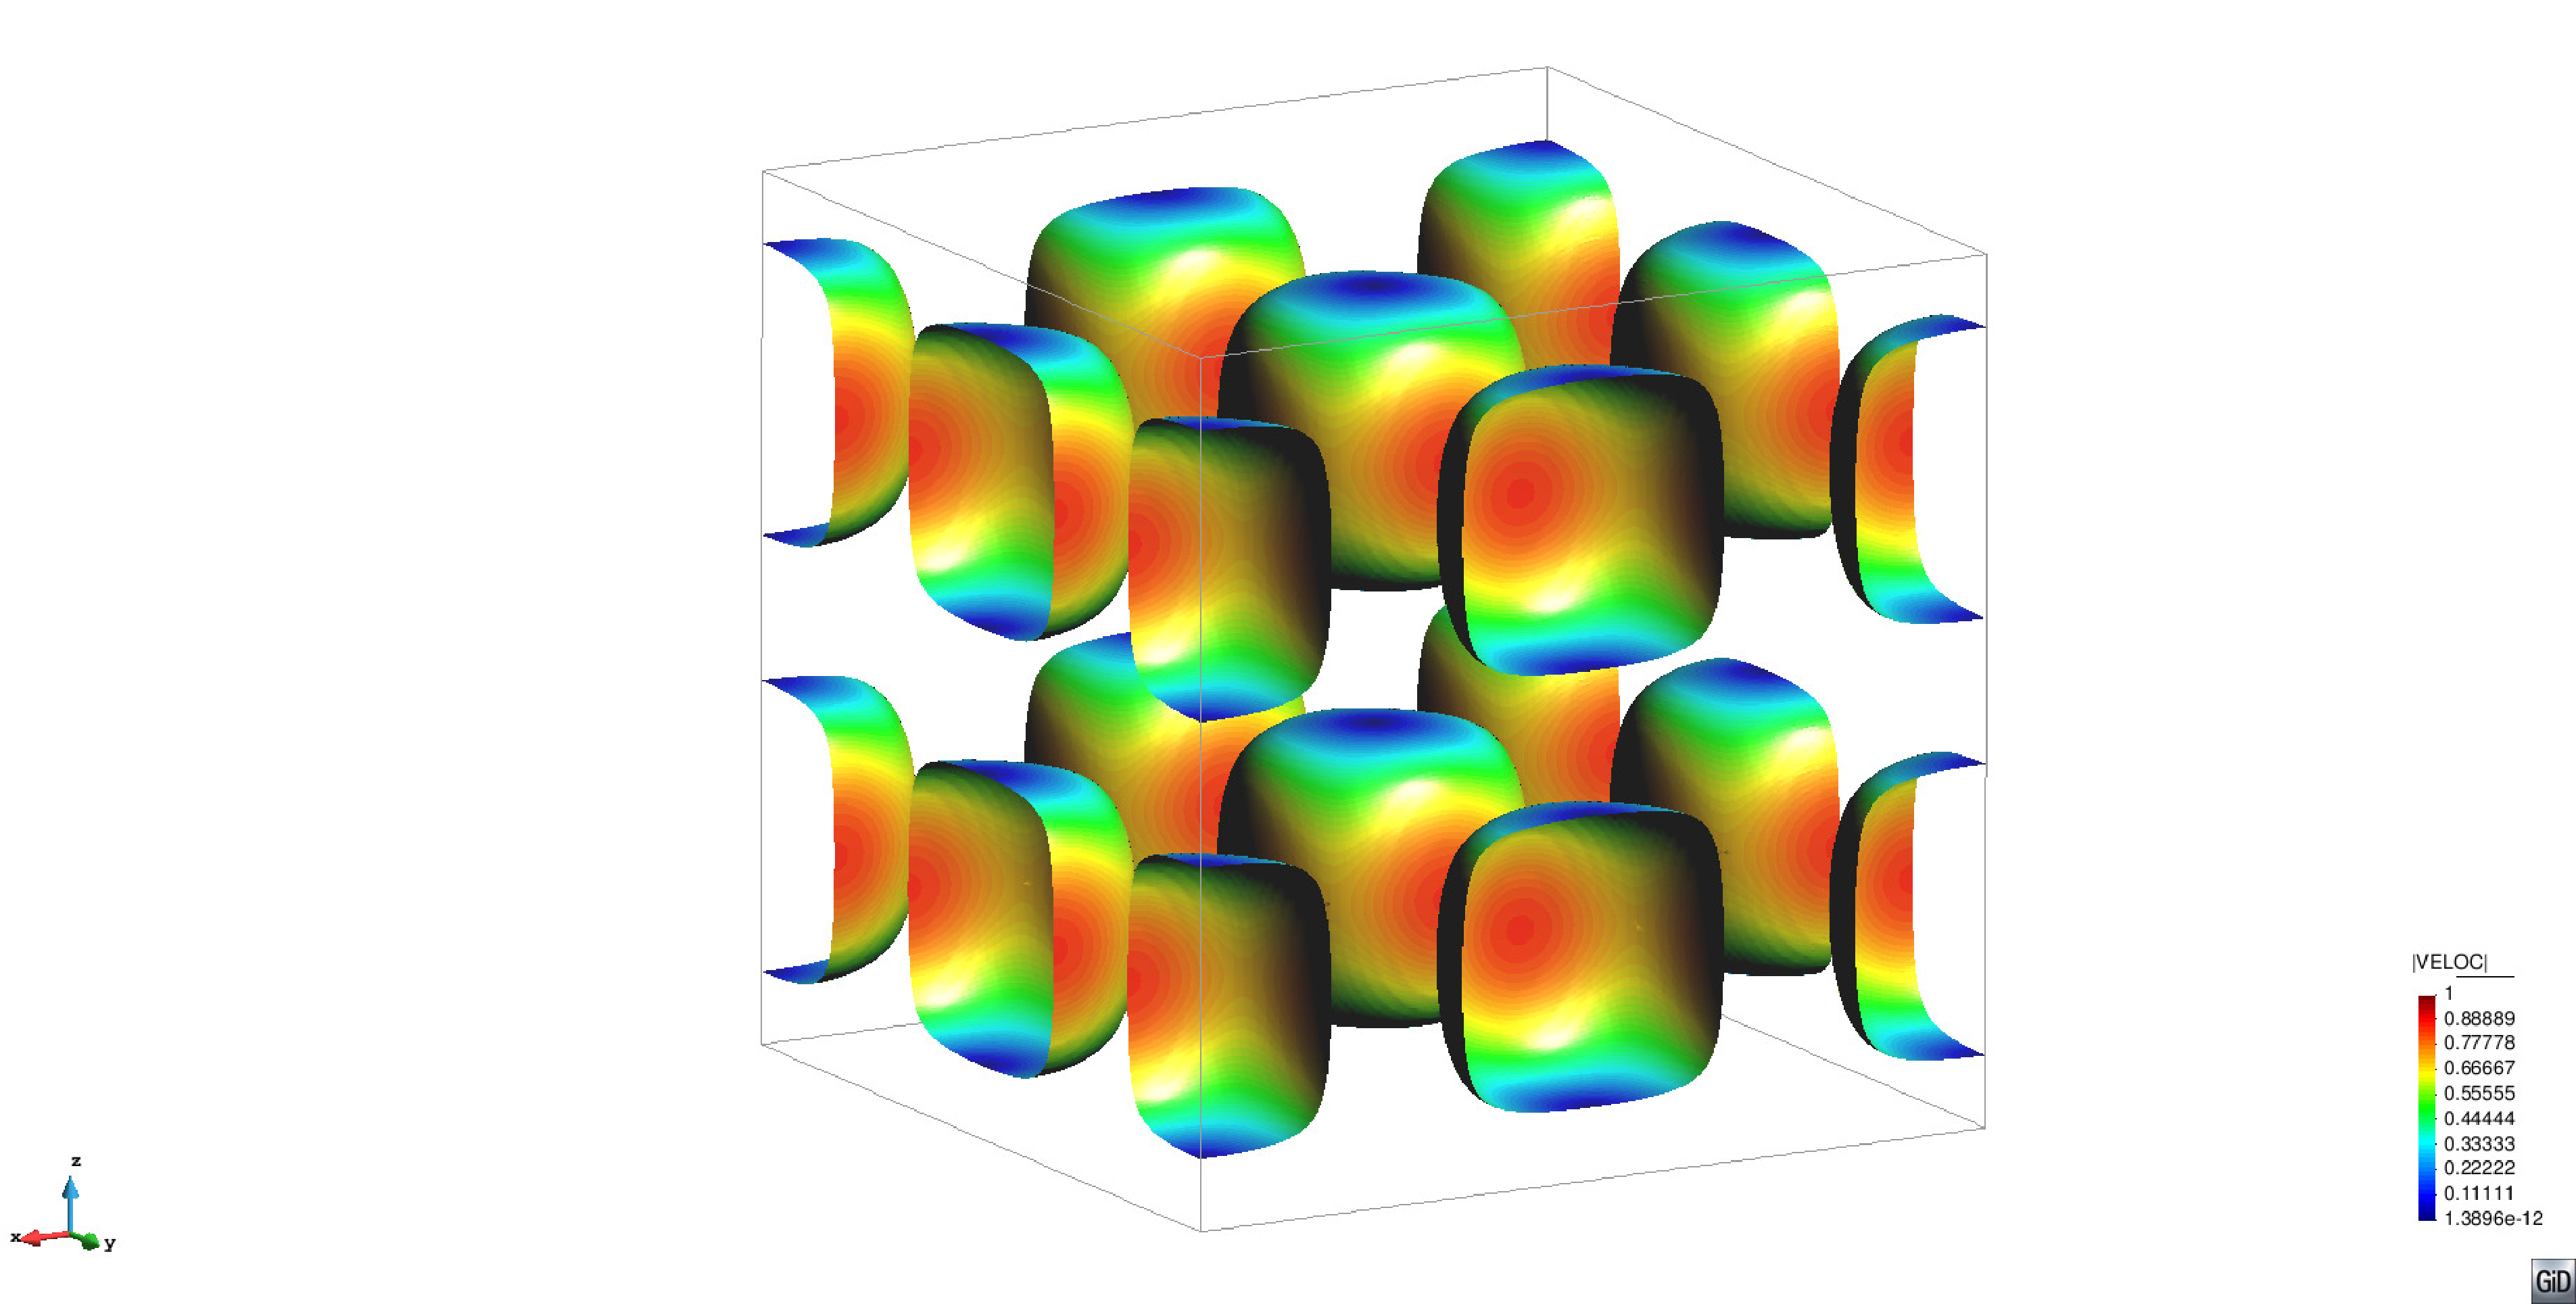
\includegraphics[trim=18cm 1cm 14cm 1cm, clip=true, width=0.45\textwidth]{Figures/isovorti_veloc_1.pdf}
	    \vspace*{-0.2cm}
	    \caption{Initial vorticity isosurface $|\omega|=1$}
	  \end{figure}}
  \only<2>{
      \vspace*{-0.3cm}
	  \begin{figure}
	    \centering	
	    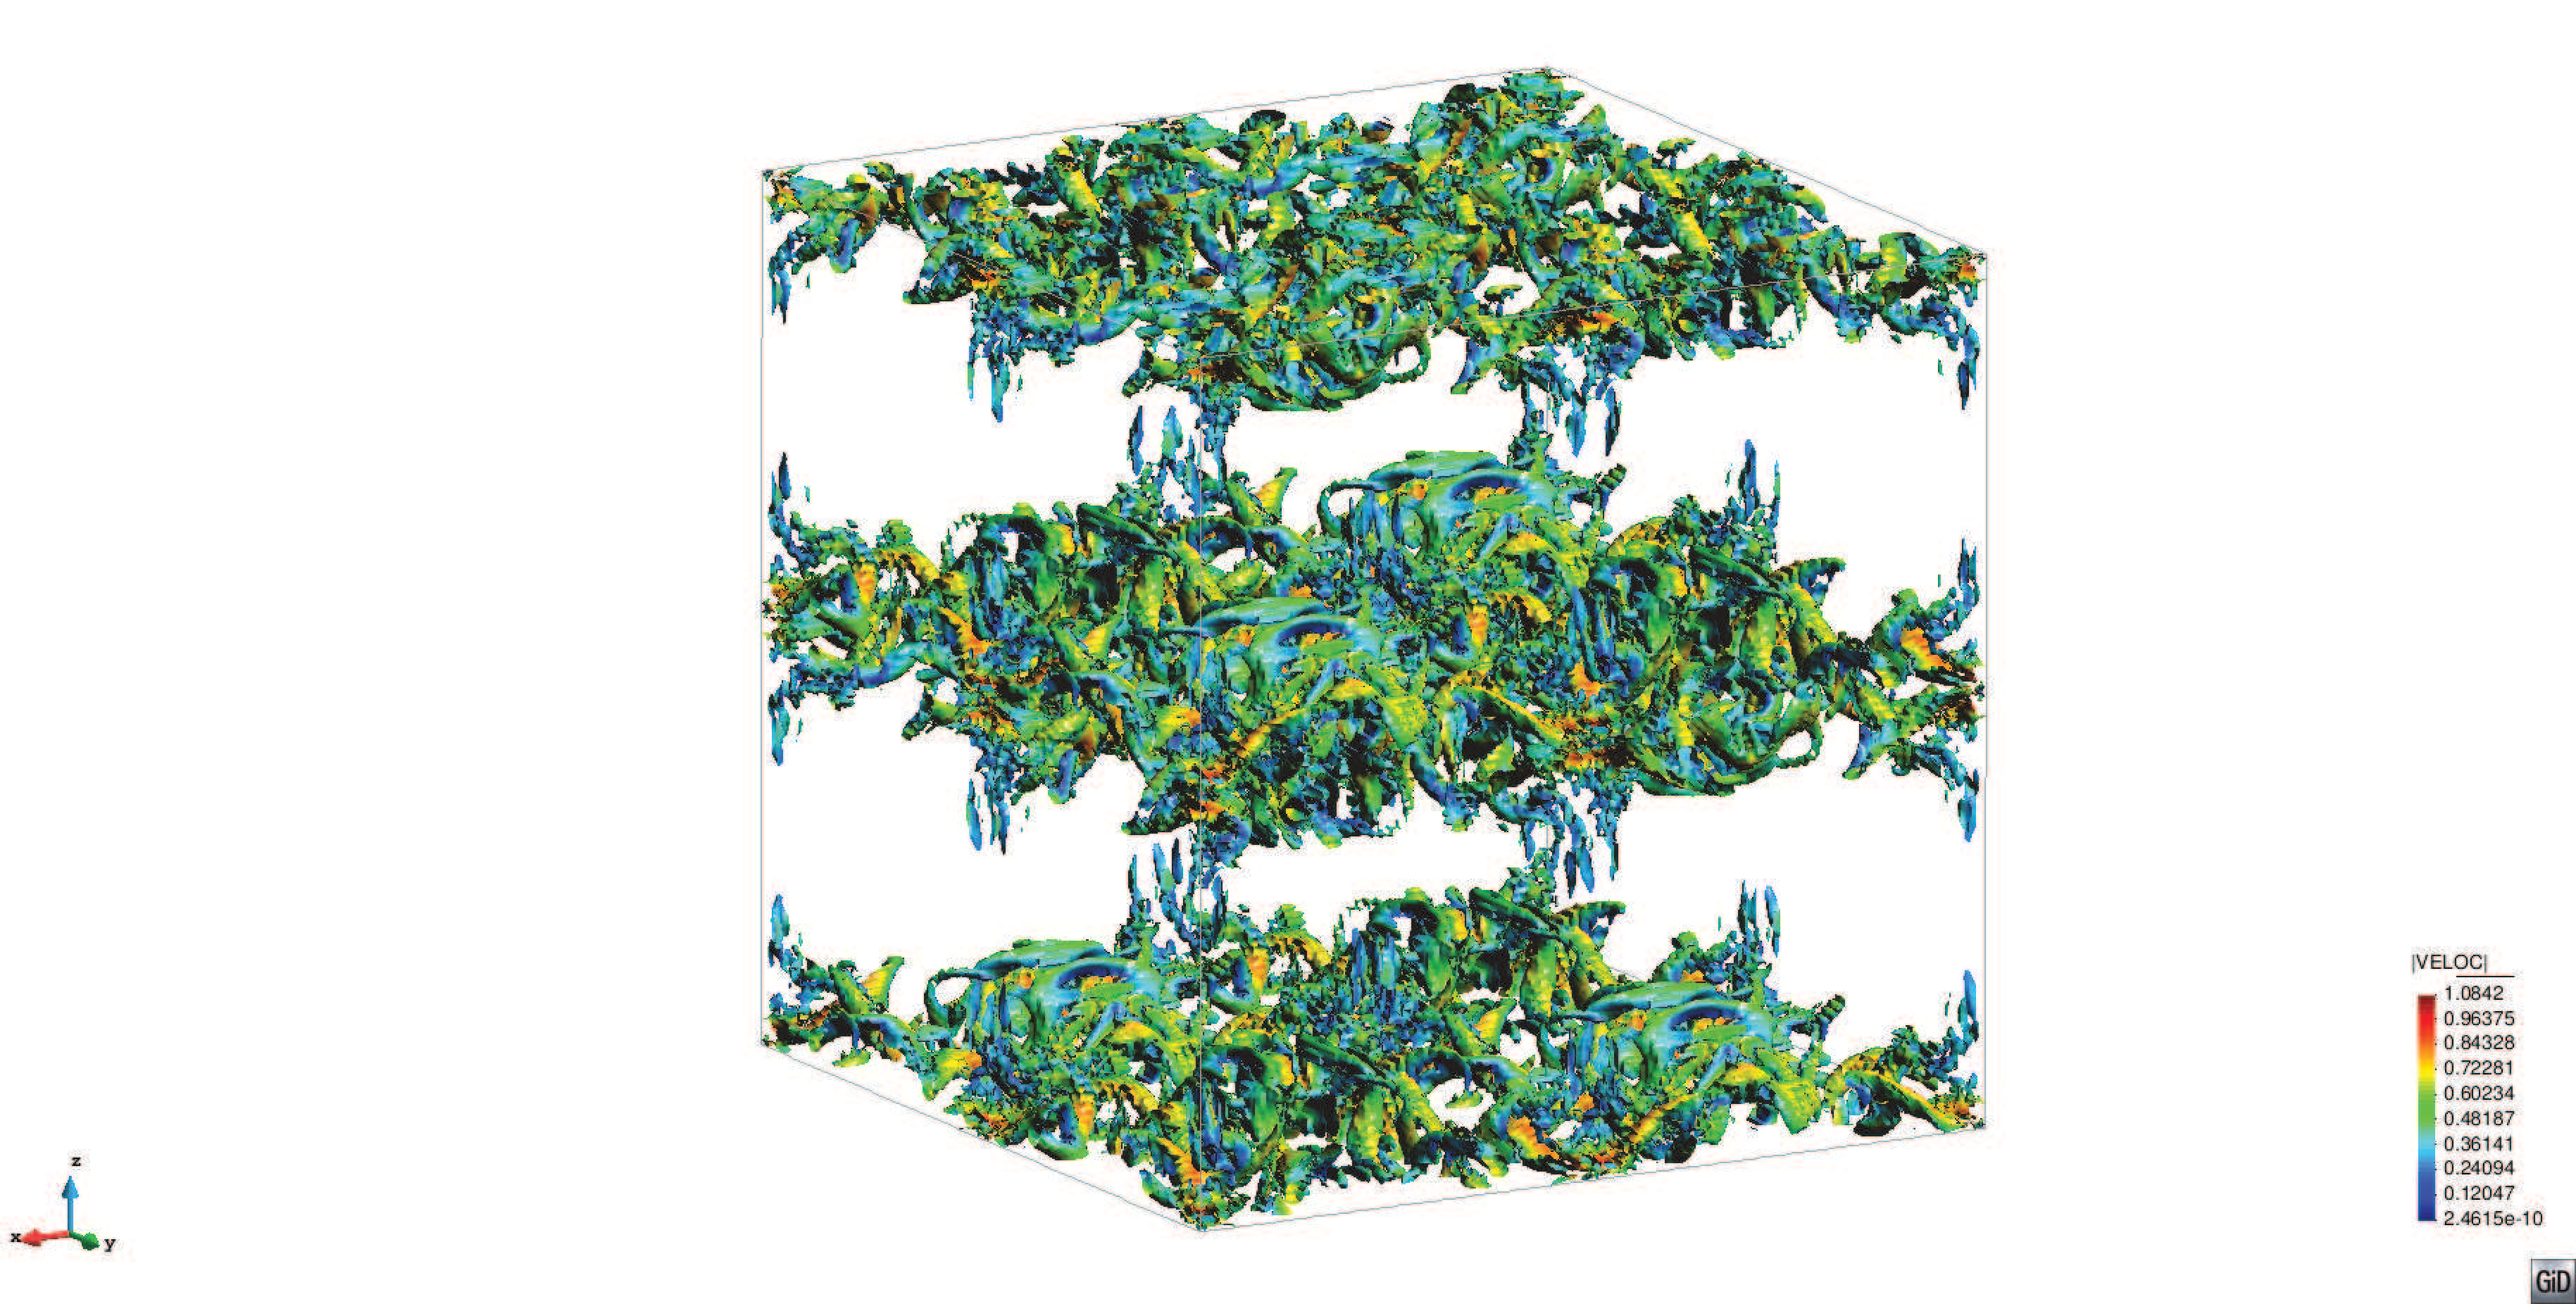
\includegraphics[trim=18cm 1cm 14cm 1cm, clip=true, width=0.45\textwidth]{Figures/isovorti_veloc_6.pdf}
	    \vspace*{-0.2cm}
	    \caption{Vorticity isosurfaces $|\omega|=9.0$}
	  \end{figure}}}
\only<3>{
\begin{figure}[h!]
\centering    
\movie[label=show3,width=1.0\textwidth,poster,autostart,showcontrols,loop]{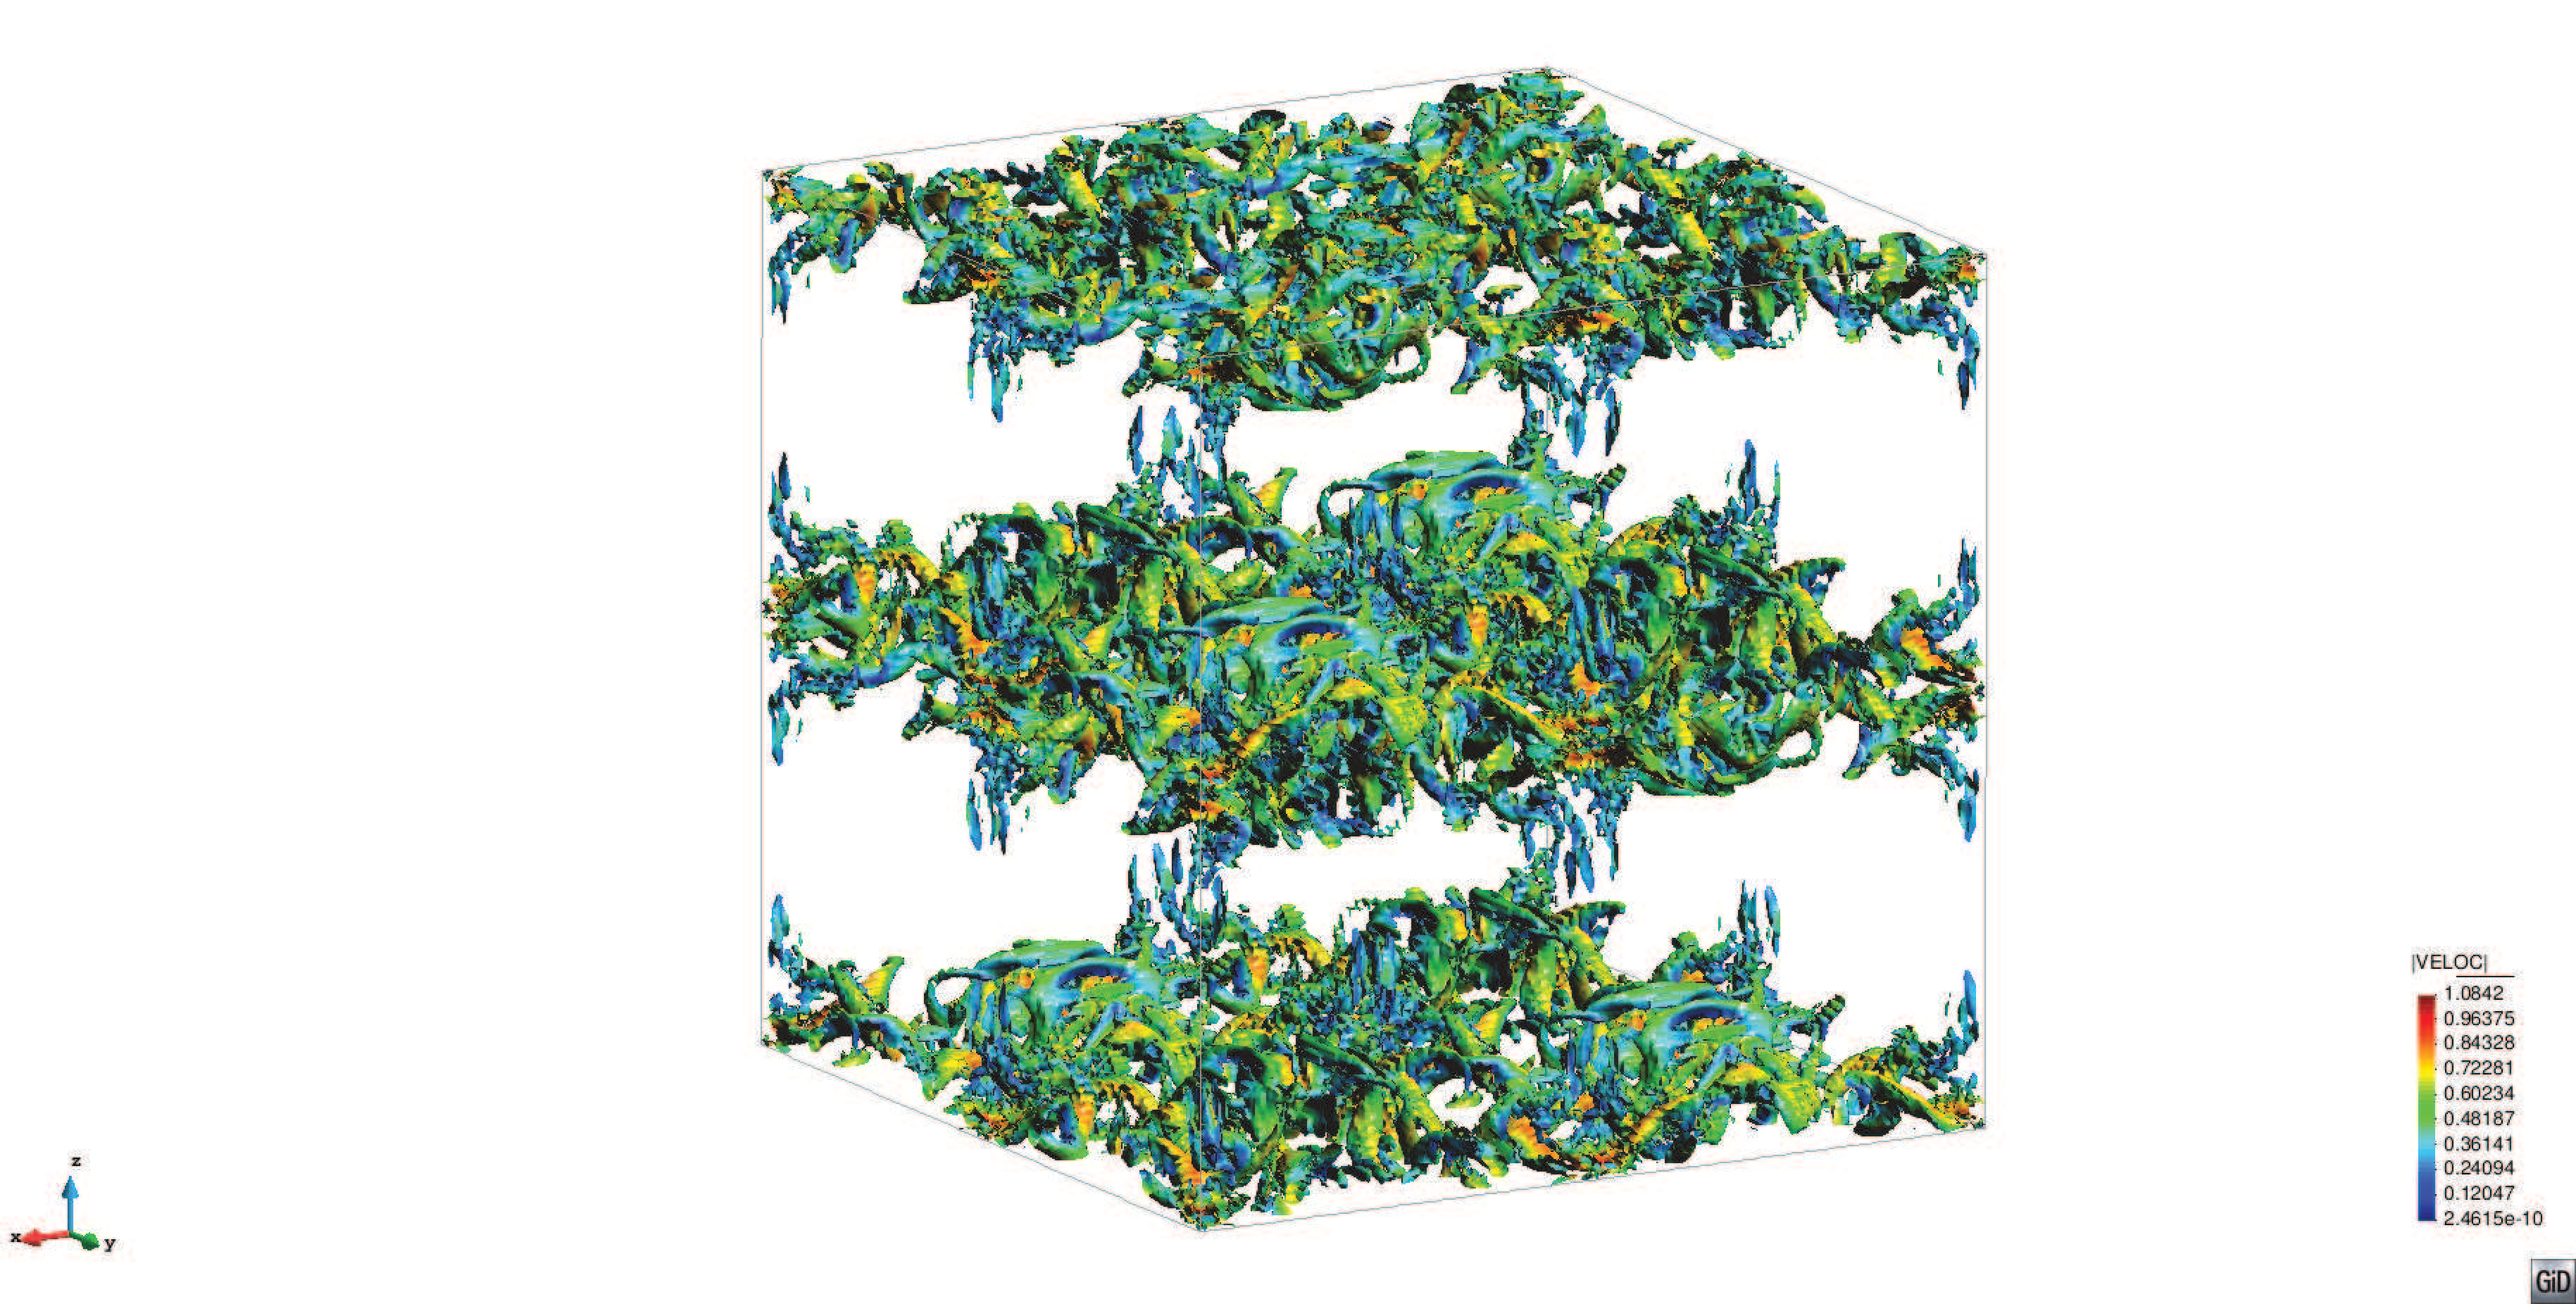
\includegraphics[width=1.0\textwidth]{Figures/isovorti_veloc_6}}{Movies/TGV.avi}
%\includemedia[activate=onclick,width=1.0\textwidth]{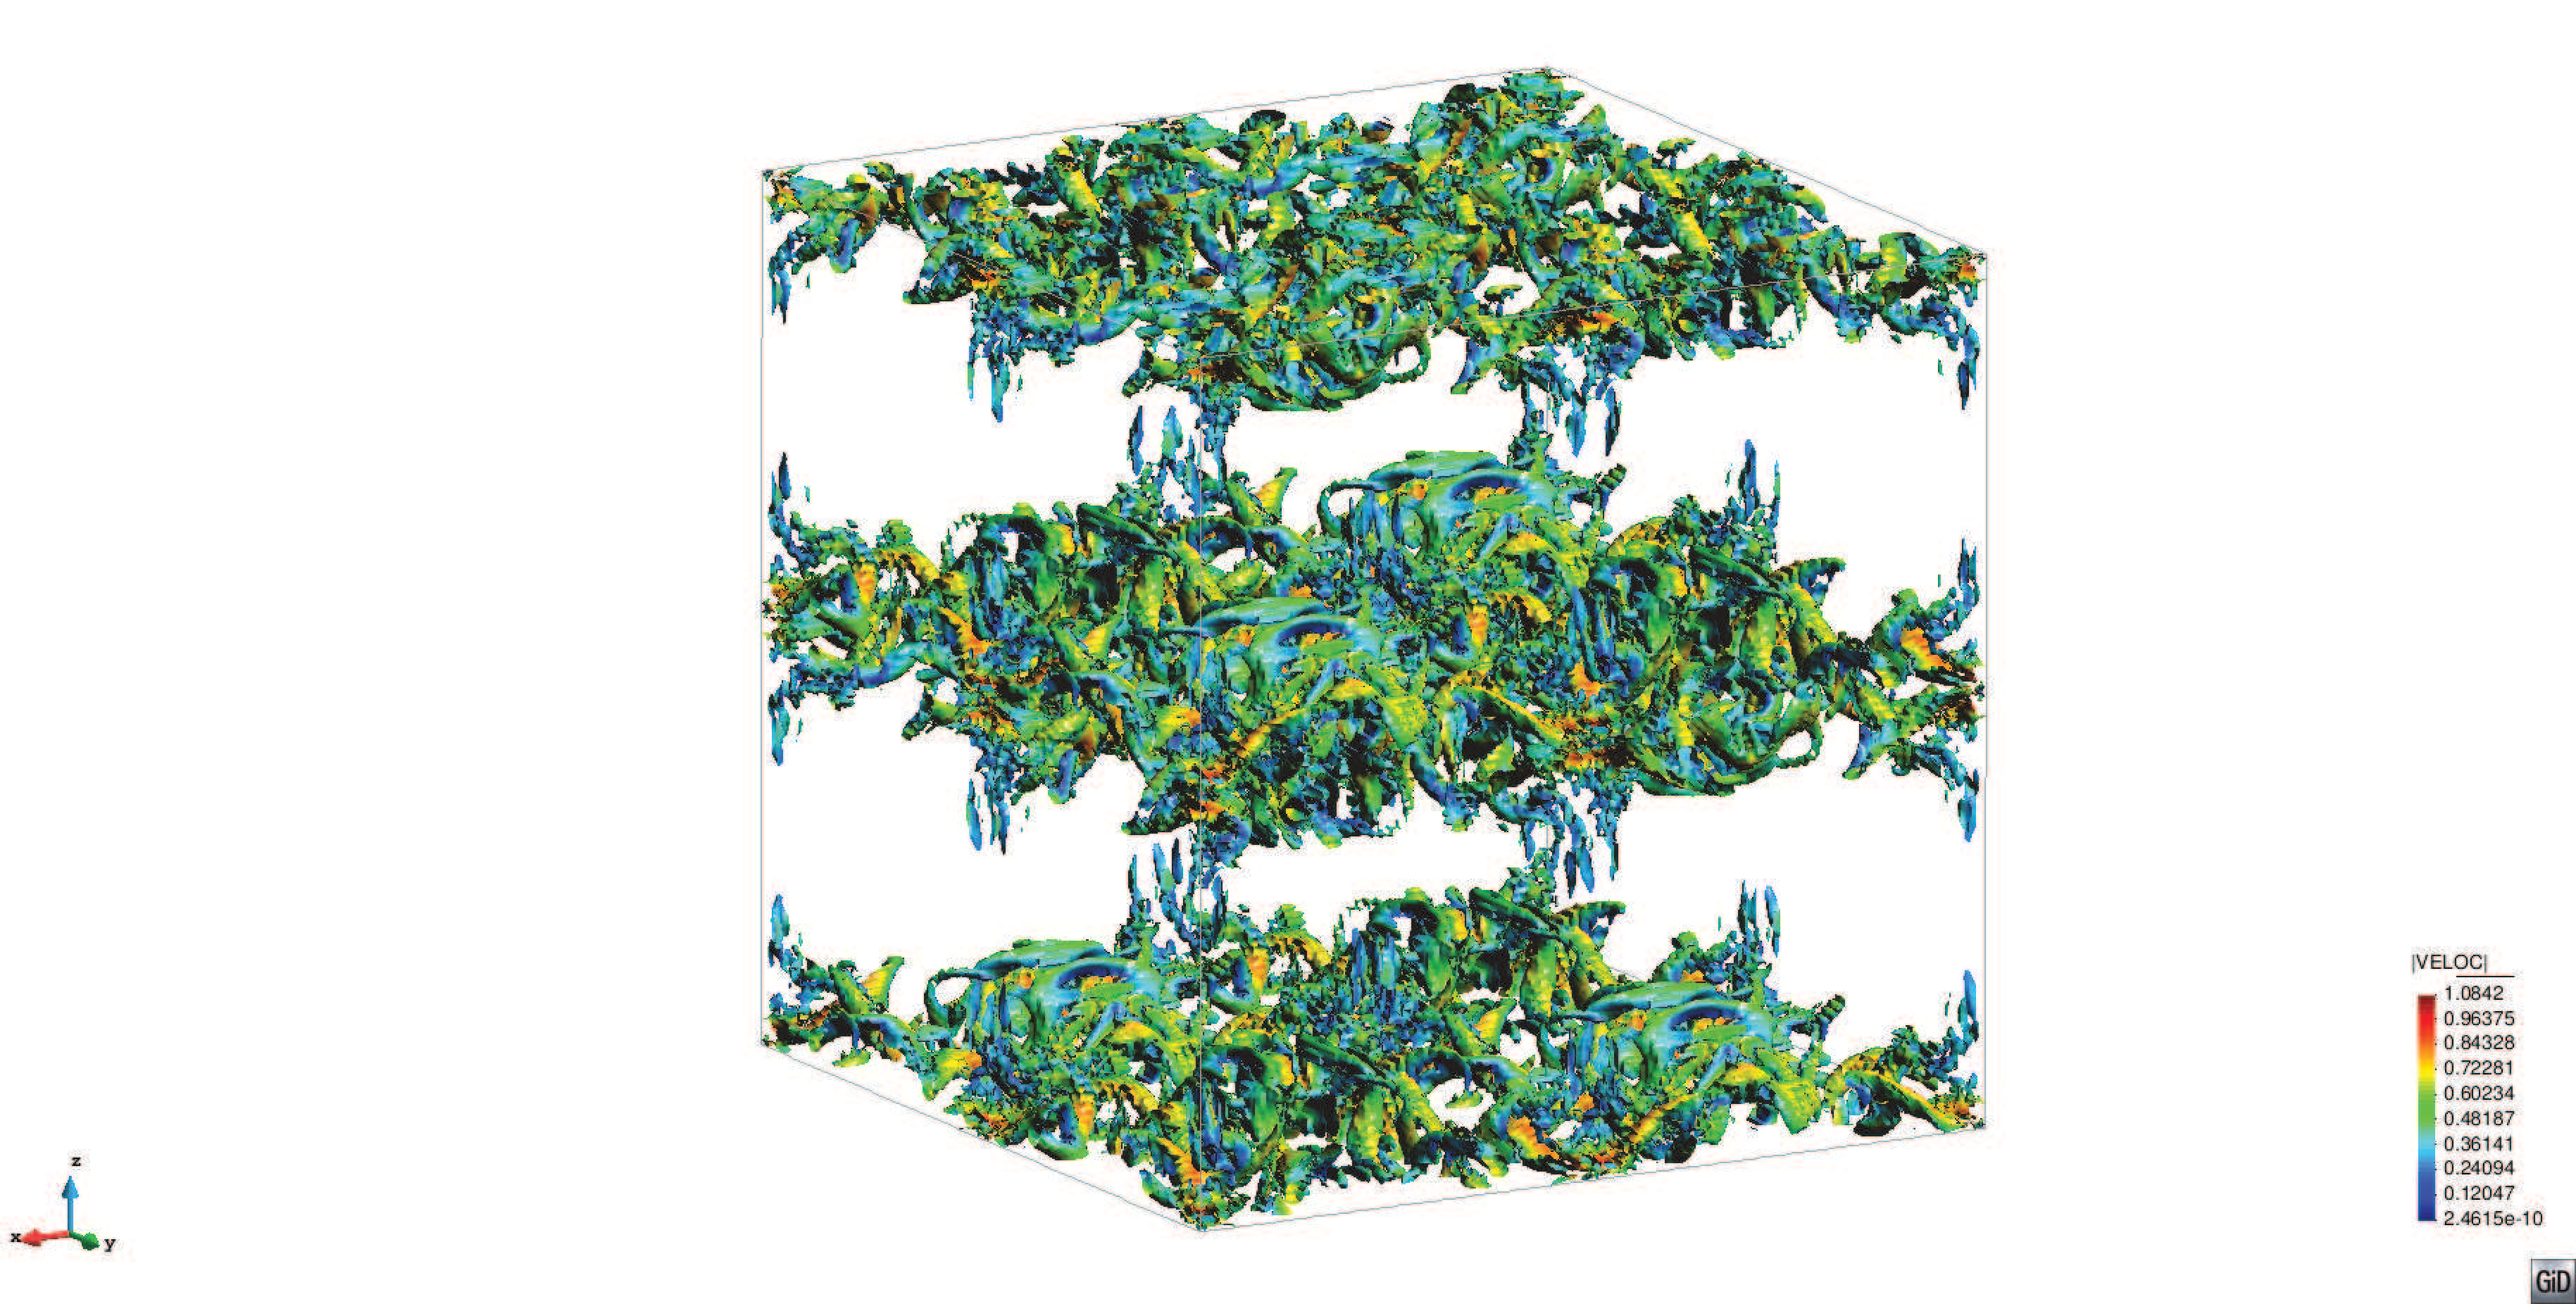
\includegraphics[width=1.0\textwidth]{Figures/isovorti_veloc_6}}{Movies/TGV.flv}
  \caption{Velocity isosurface}
 \end{figure} }
\end{frame}
%----------------------------------------------------------------------------------------
\begin{frame}
 \frametitle{TGV {\small Taylor-Green Vortex flow}}
 \textbf{Energy dissipation rate (refinement):}
 \vspace*{-1.0cm}
 \begin{columns}
   \begin{column}{0.5\textwidth}
   \begin{figure}
     \centering	
     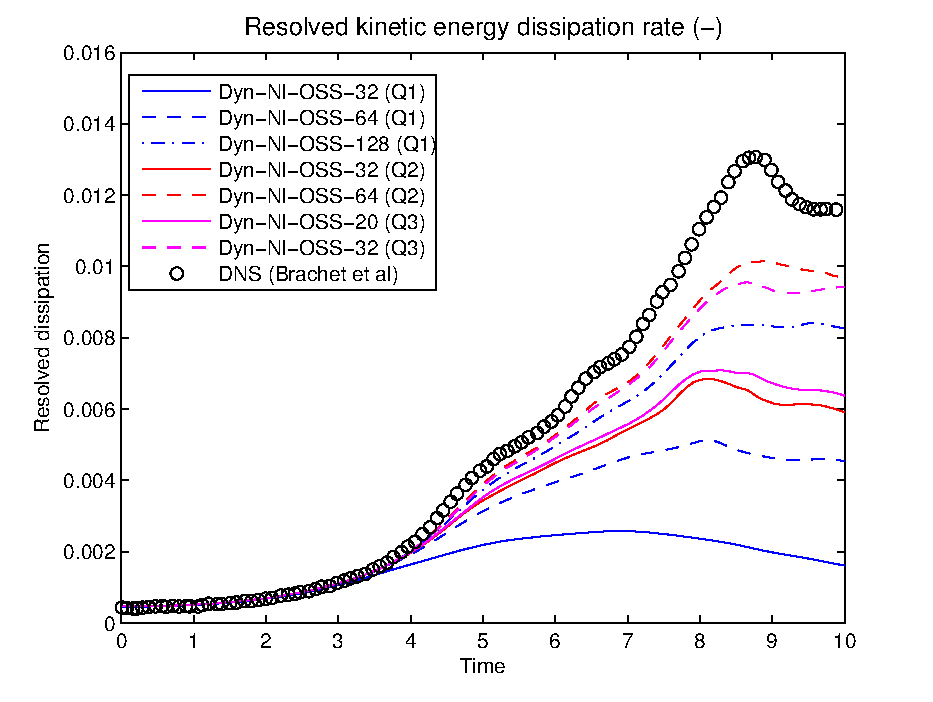
\includegraphics[width=1.1\textwidth]{Figures/ens_hp_10_new_resolved.pdf}
     \vspace*{-0.8cm}
     \caption{Resolved scales}
   \end{figure}
   \end{column}
   \begin{column}{0.5\textwidth}
   \begin{figure}
     \centering	
     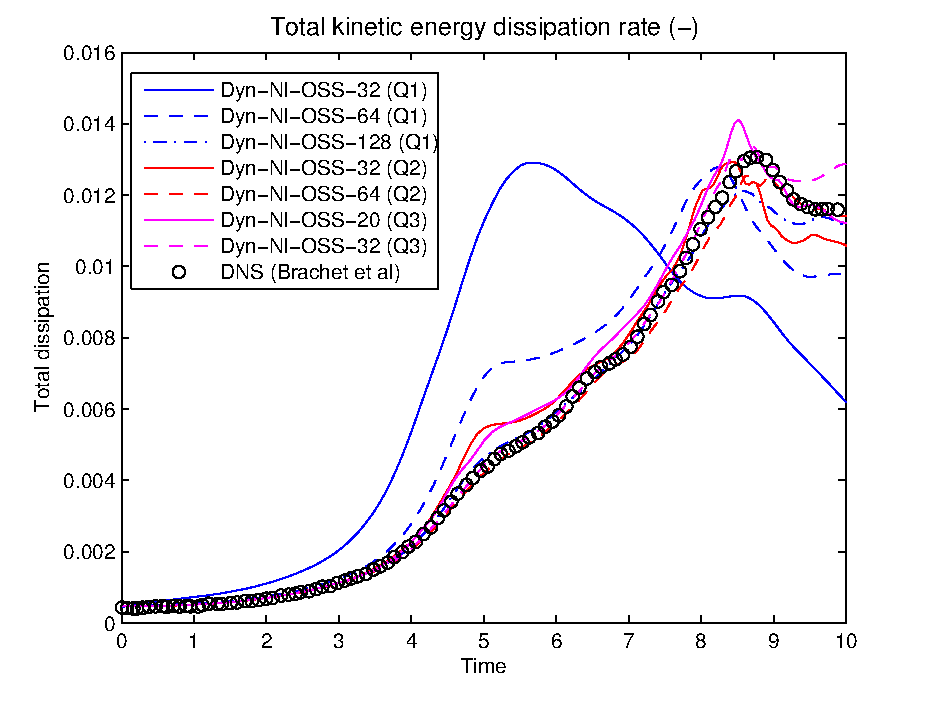
\includegraphics[width=1.1\textwidth]{Figures/ens_hp_10_new_total.pdf}
     \vspace*{-0.8cm}
     \caption{Total}
   \end{figure}
   \end{column}
 \end{columns}
 \begin{overlayarea}{\textwidth}{1.5cm}
 \only<2->{
 \vspace*{-0.3cm}
 \begin{itemize}
  	\item \alert<2>{Good agreement with the DNS} taking account the subscales
  	\only<3->{\item \alert<3>{More accurate results increasing the order} of approximation}
  \end{itemize}}
  \end{overlayarea}
\end{frame}
%----------------------------------------------------------------------------------------
\addtocounter{framenumber}{-1}
\begin{frame}
 \frametitle{TGV {\small Taylor-Green Vortex flow}}
 \vfill
 {\large
 \begin{itemize}
 	\item All results until now are compared against \textbf{DNS}
 \end{itemize}
 \vspace*{0.5cm}
  \begin{itemize}
  	\item Are our methods comparable with \textbf{LES} models?
 \end{itemize}}
 \vfill
\end{frame}
%----------------------------------------------------------------------------------------
\begin{frame}
 \frametitle{TGV {\small Taylor-Green Vortex flow}}
 \textbf{Energy dissipation rate (against LES model):}
 \vspace*{-1.0cm}
 \begin{columns}
   \begin{column}{0.5\textwidth}
   \begin{figure}
     \centering	
     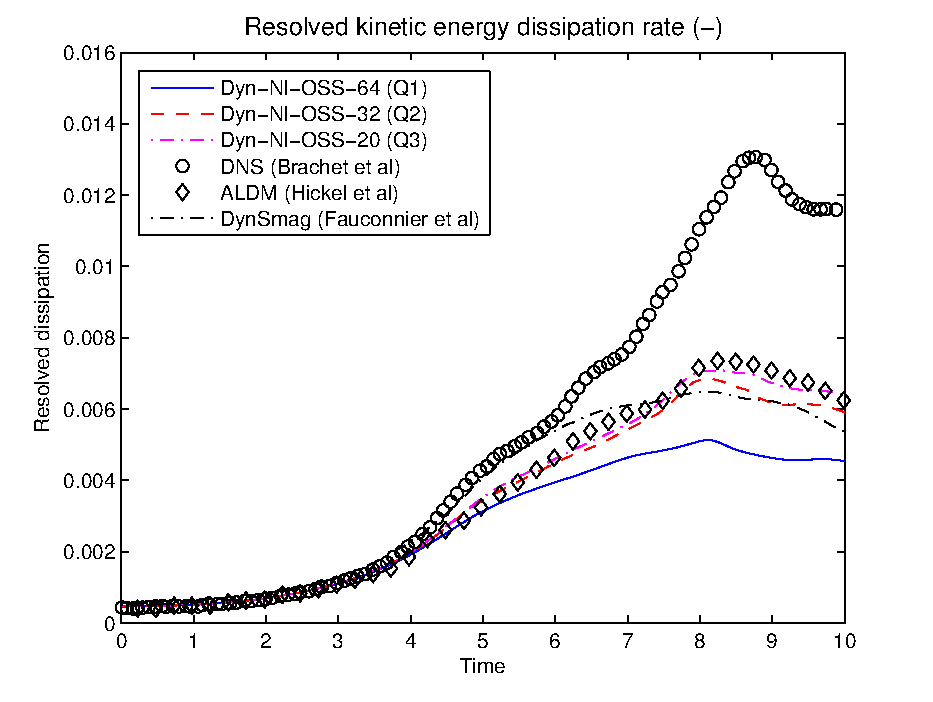
\includegraphics[width=1.1\textwidth]{Figures/ens_64dofs_dynsmag_resolved.pdf}
     \vspace*{-0.8cm}
     \caption{Resolved scales}
   \end{figure}
   \end{column}
   \begin{column}{0.5\textwidth}
   \begin{figure}
     \centering	
     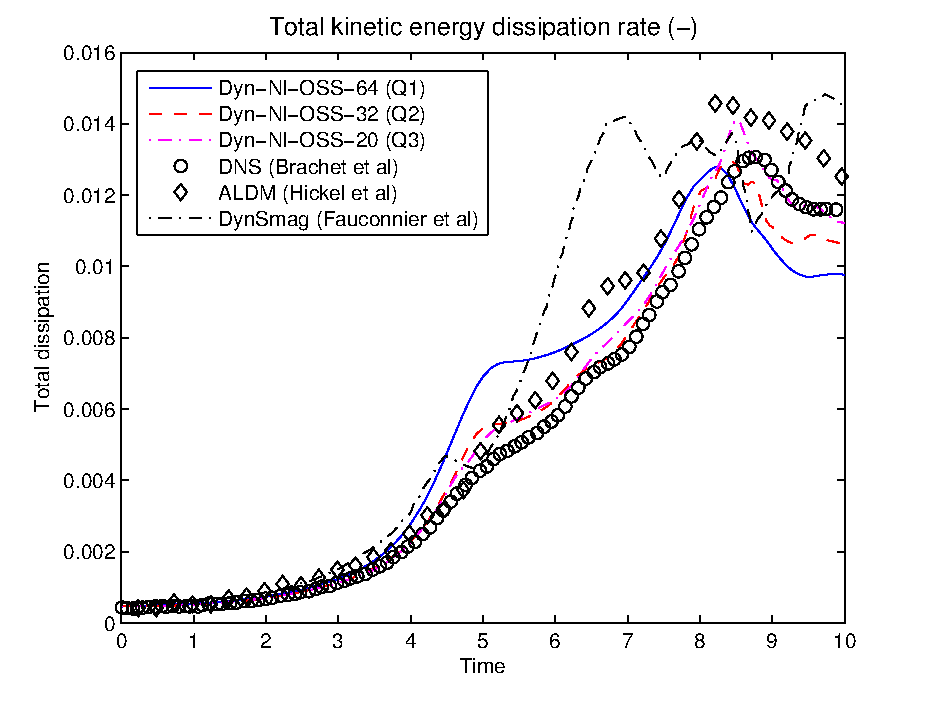
\includegraphics[width=1.1\textwidth]{Figures/ens_64dofs_dynsmag_total.pdf}
     \vspace*{-0.8cm}
     \caption{Total}
   \end{figure}
   \end{column}
 \end{columns}
 \begin{overlayarea}{\textwidth}{1.5cm}
  \only<2->{
  \vspace*{-0.3cm}
 \begin{itemize}
  	\item \alert<2>{Good agreement with the LES models} on resolved scales
  	\only<3->{\item \alert<3>{Better results than LES models} adding subscales counterpart}
  \end{itemize}}
  \end{overlayarea}
\end{frame}

%=========================================================================================
% 2.3.3.TCF
% ----------------------------------------------------------------------------
\subsubsection{TCF}
\begin{frame}[t]
\frametitle{TCF {\small Turbulent Channel Flow}}
\only<1>{
\textbf{Problem setting:}
\begin{itemize}
  	\item Wall bounded flow
    \item $Re_\tau=180$ and $Re_\tau=395$
    \item Mesh resolution: $32^3-Q1$ (stretched elements near the wall)
  \end{itemize}
  \begin{figure}
    \centering	
    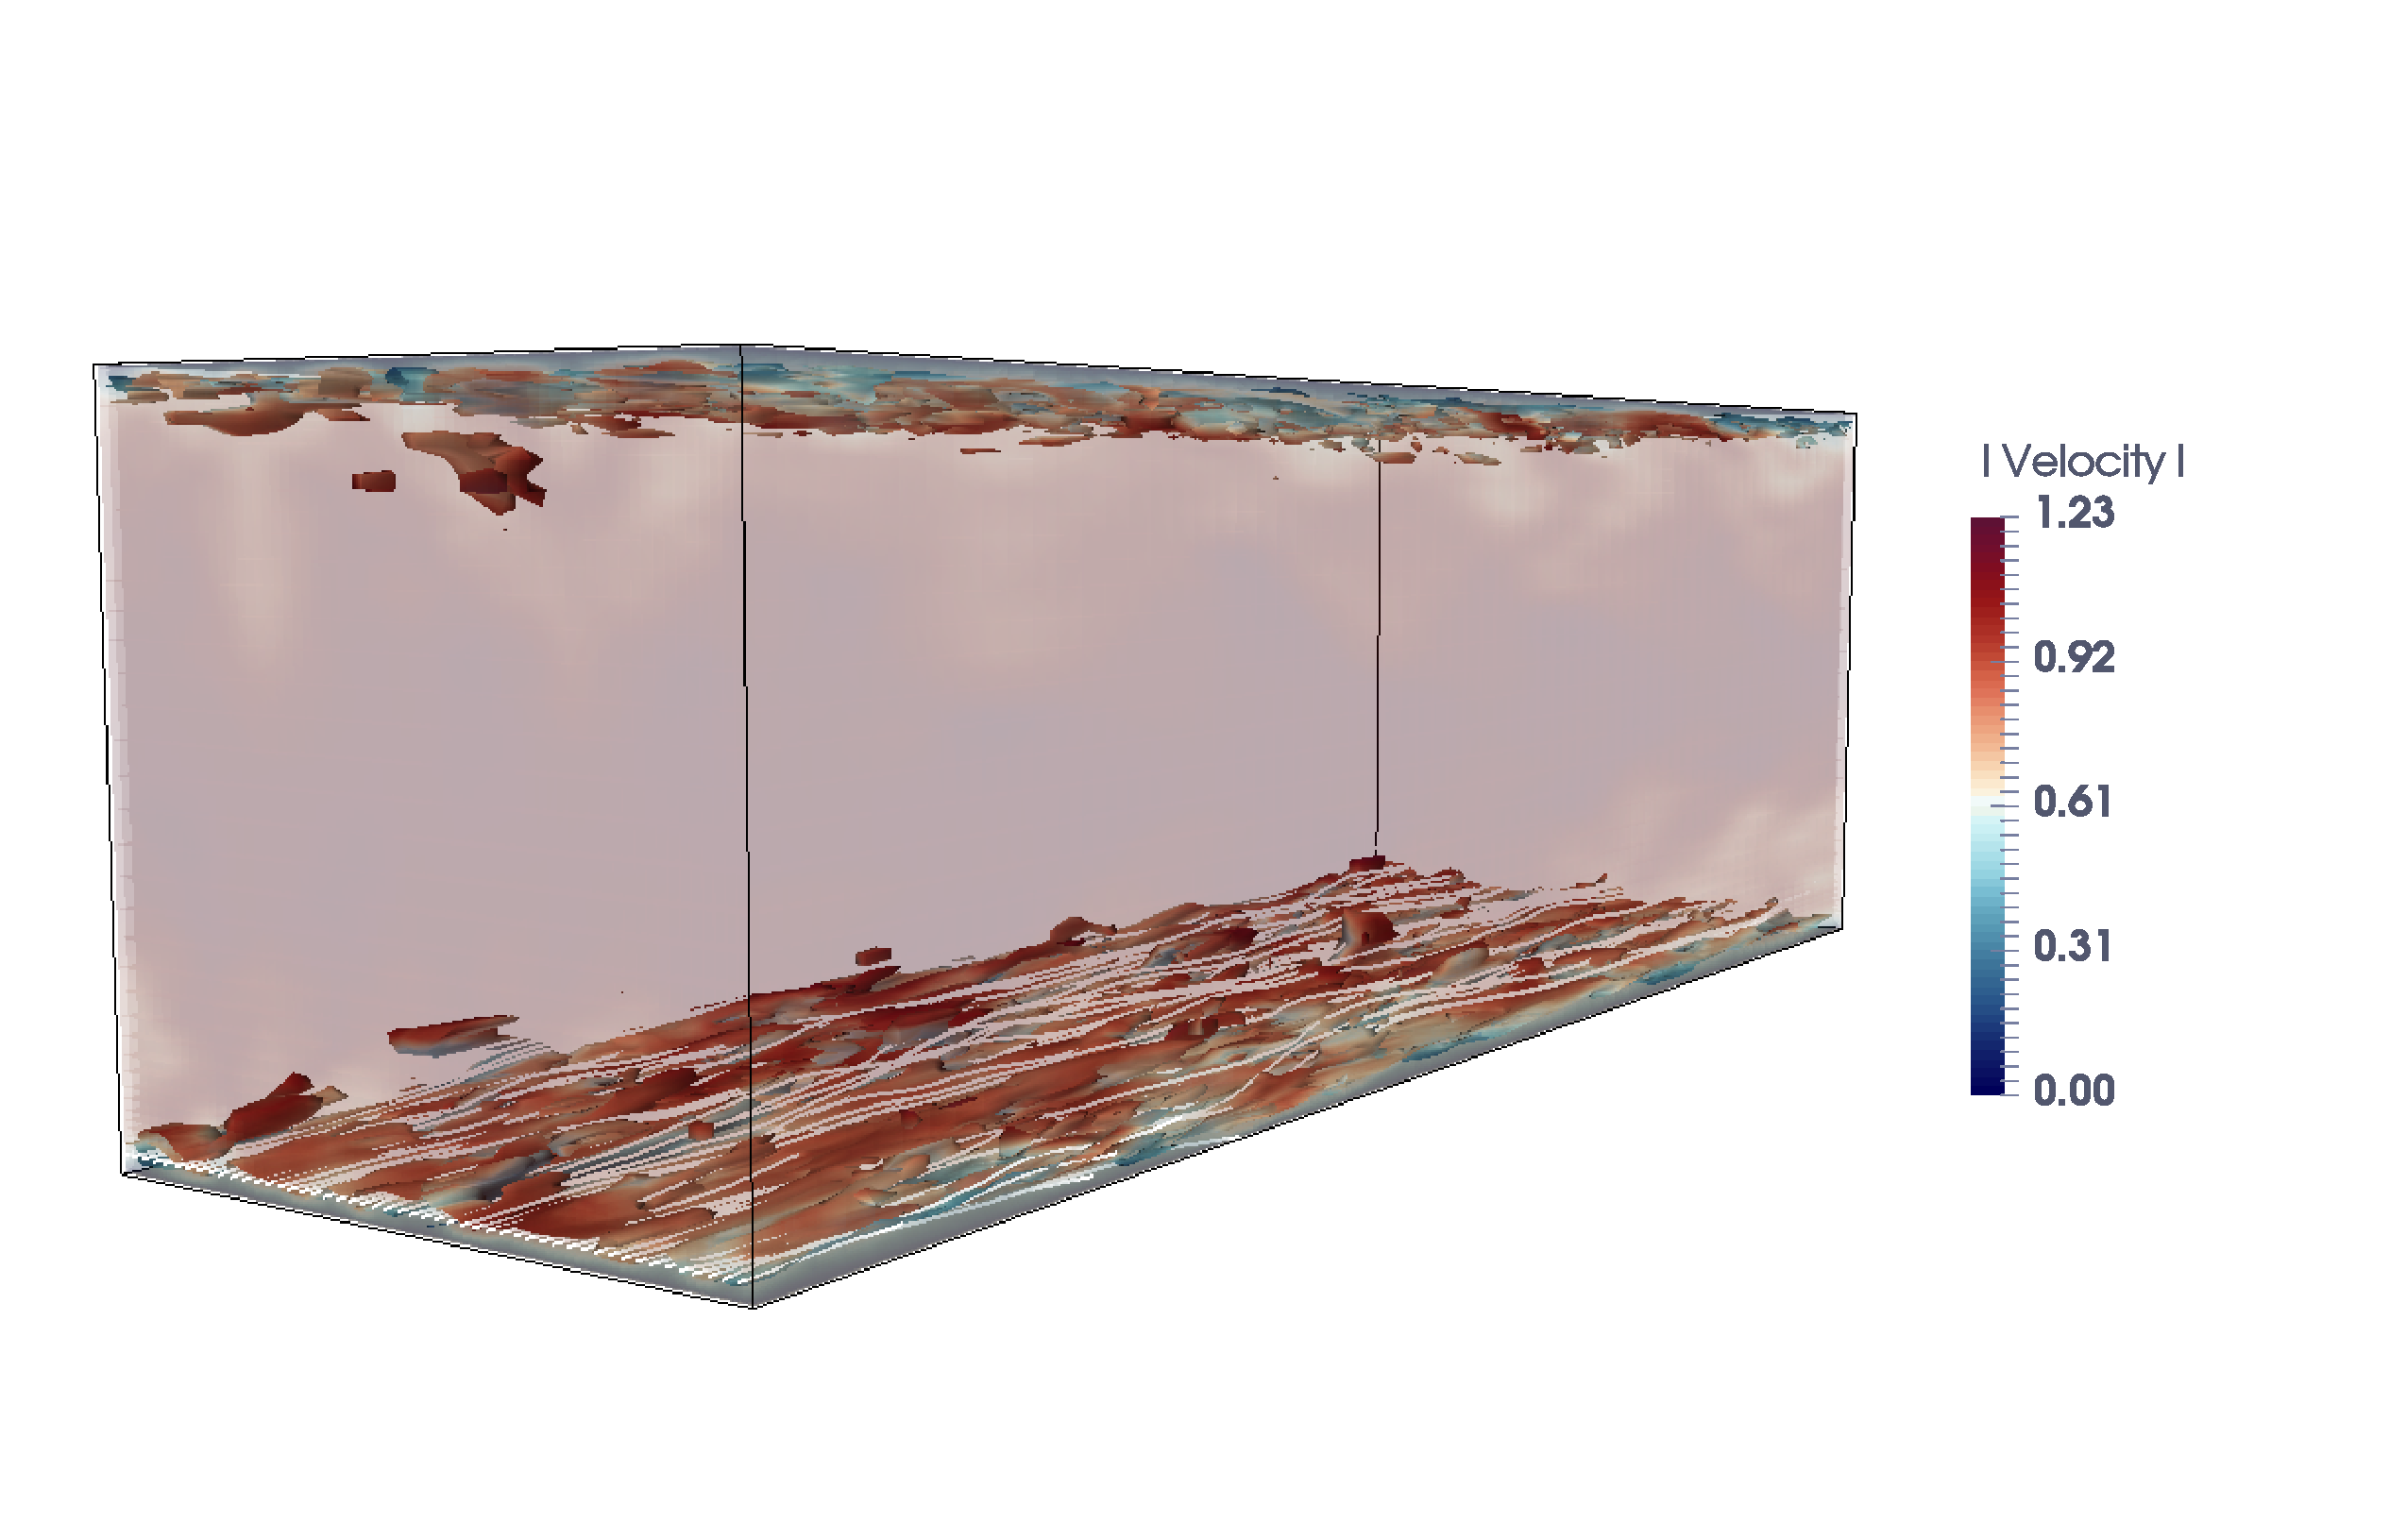
\includegraphics[width=0.8\textwidth,clip=true,trim=0cm 0cm 8cm  5cm]{Figures/cha395_32el_70}
  \end{figure}}
\only<2>{
\begin{figure}[h!]
\centering    
\movie[label=show3,width=1.0\textwidth,poster,autostart,showcontrols,loop]{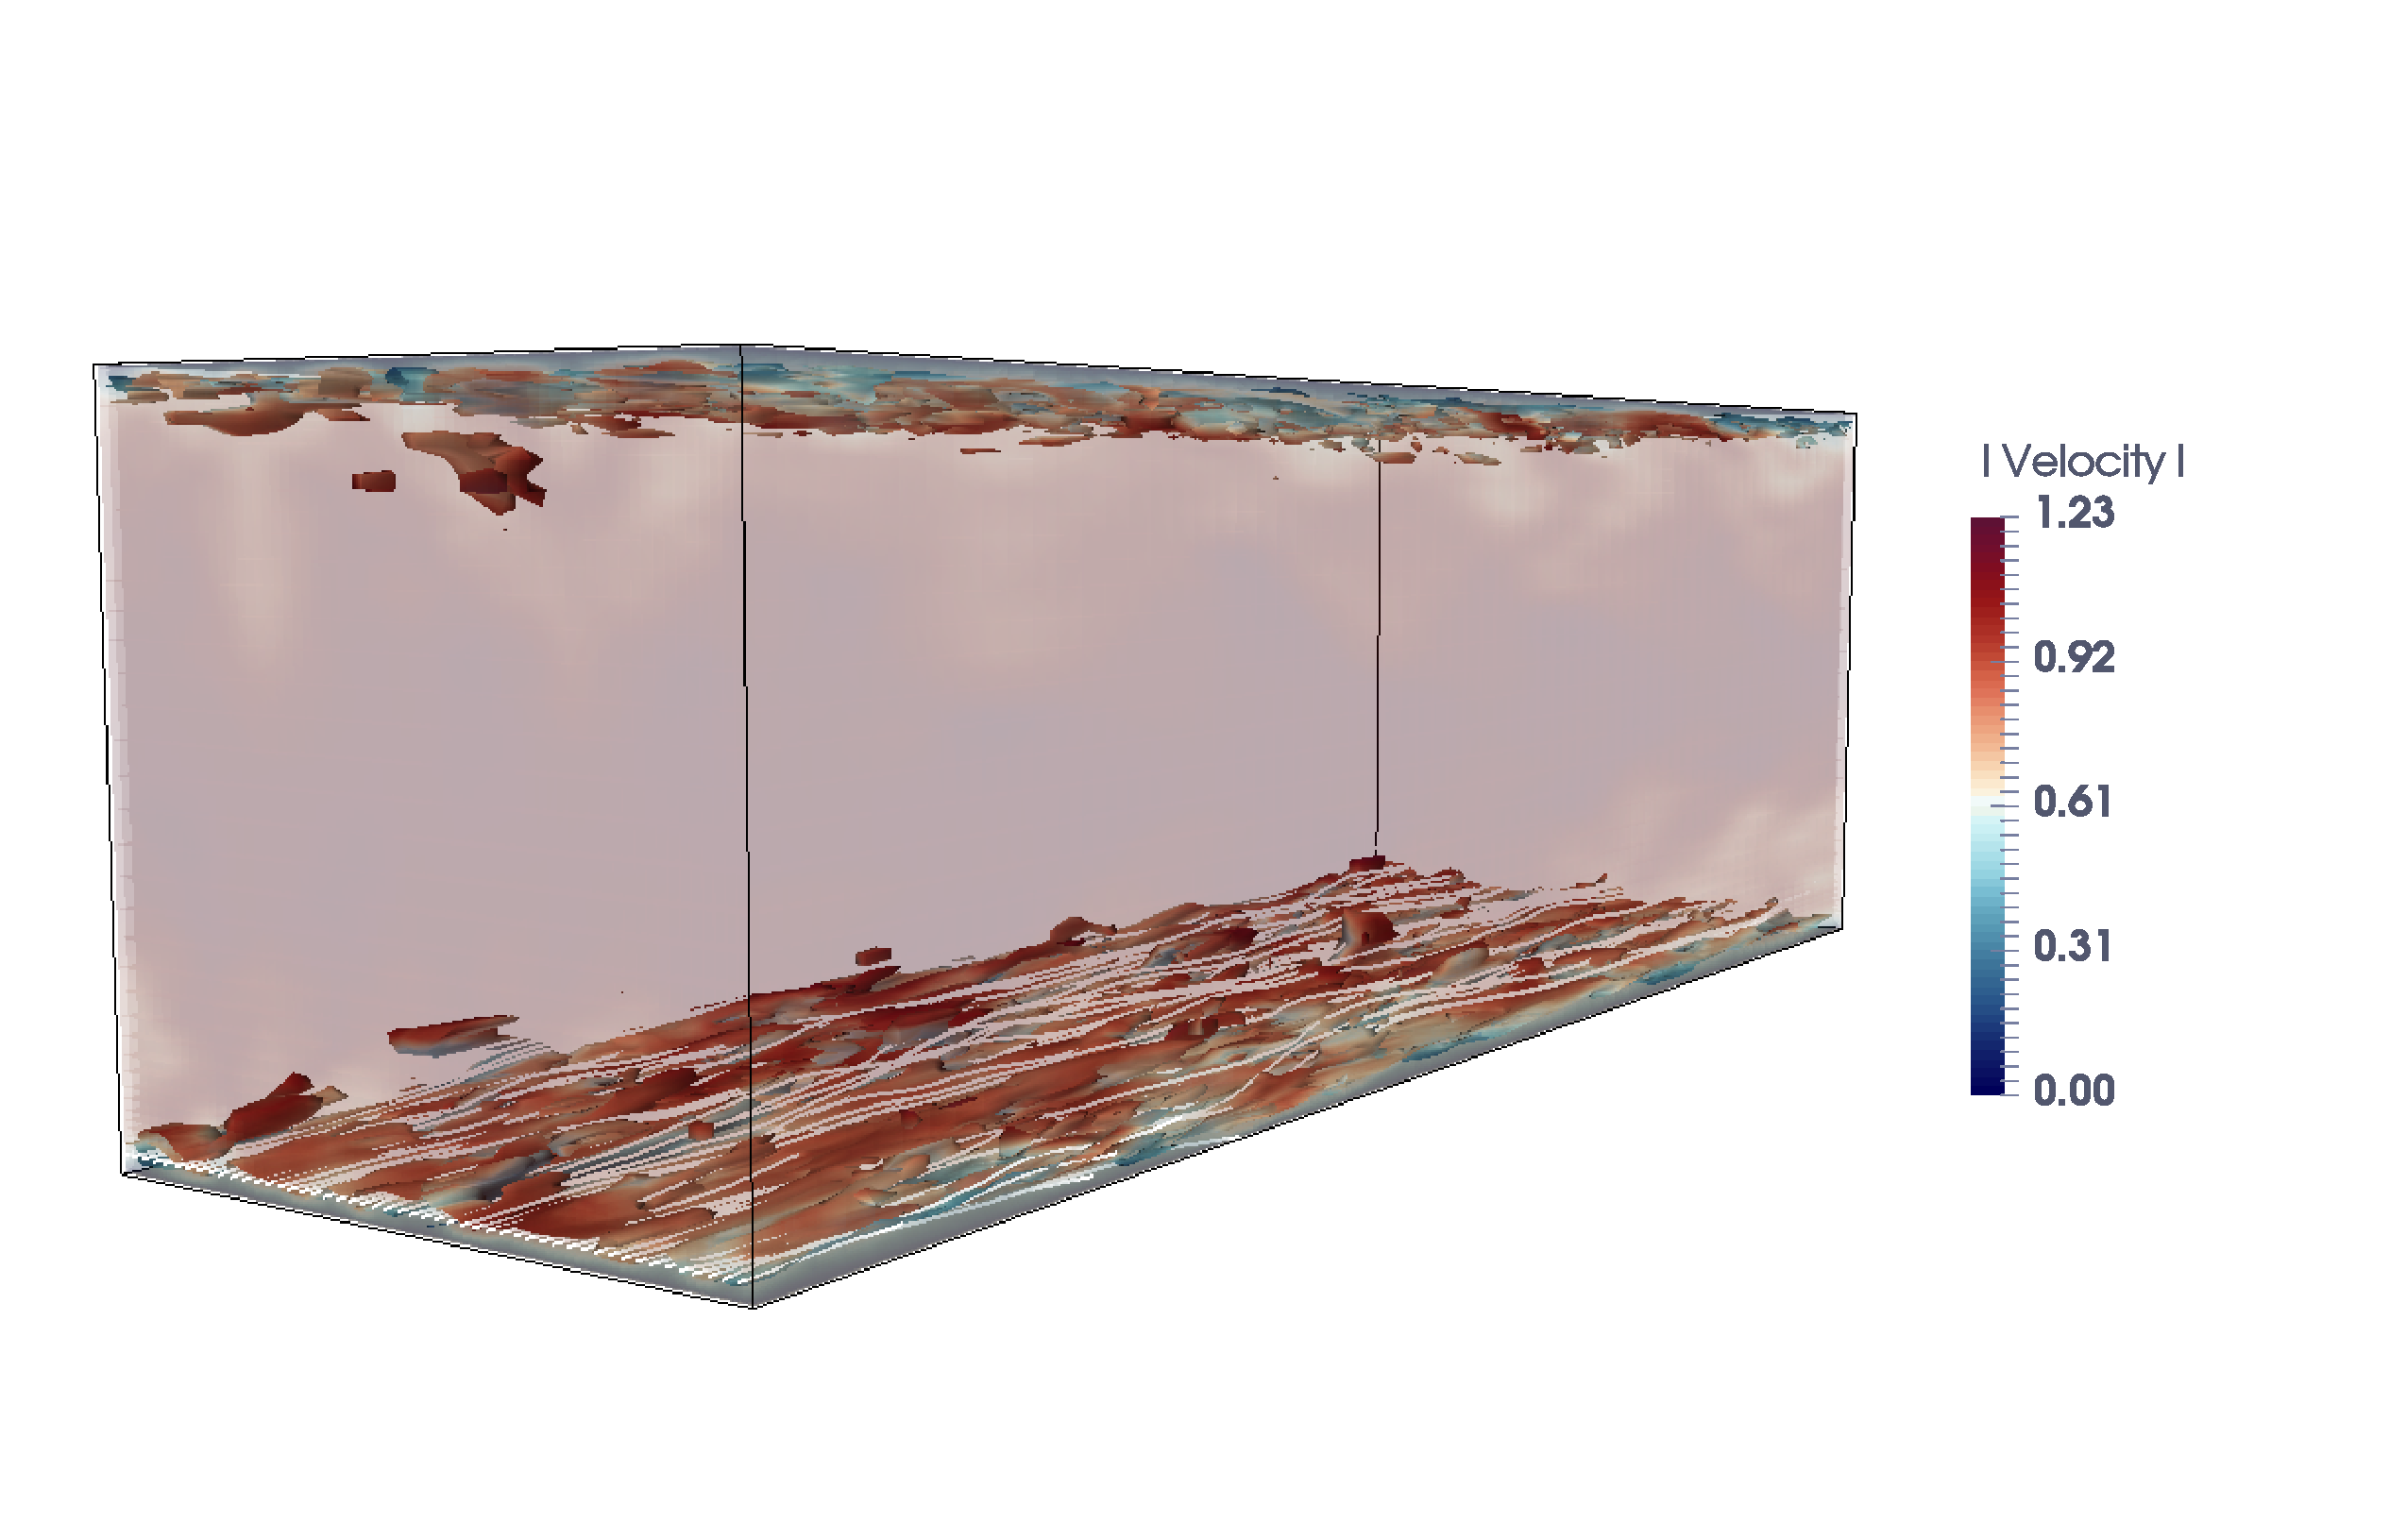
\includegraphics[width=1.0\textwidth]{Figures/cha395_32el_70}}{Movies/TCF.avi}
%\includemedia[activate=onclick,width=1.0\textwidth]{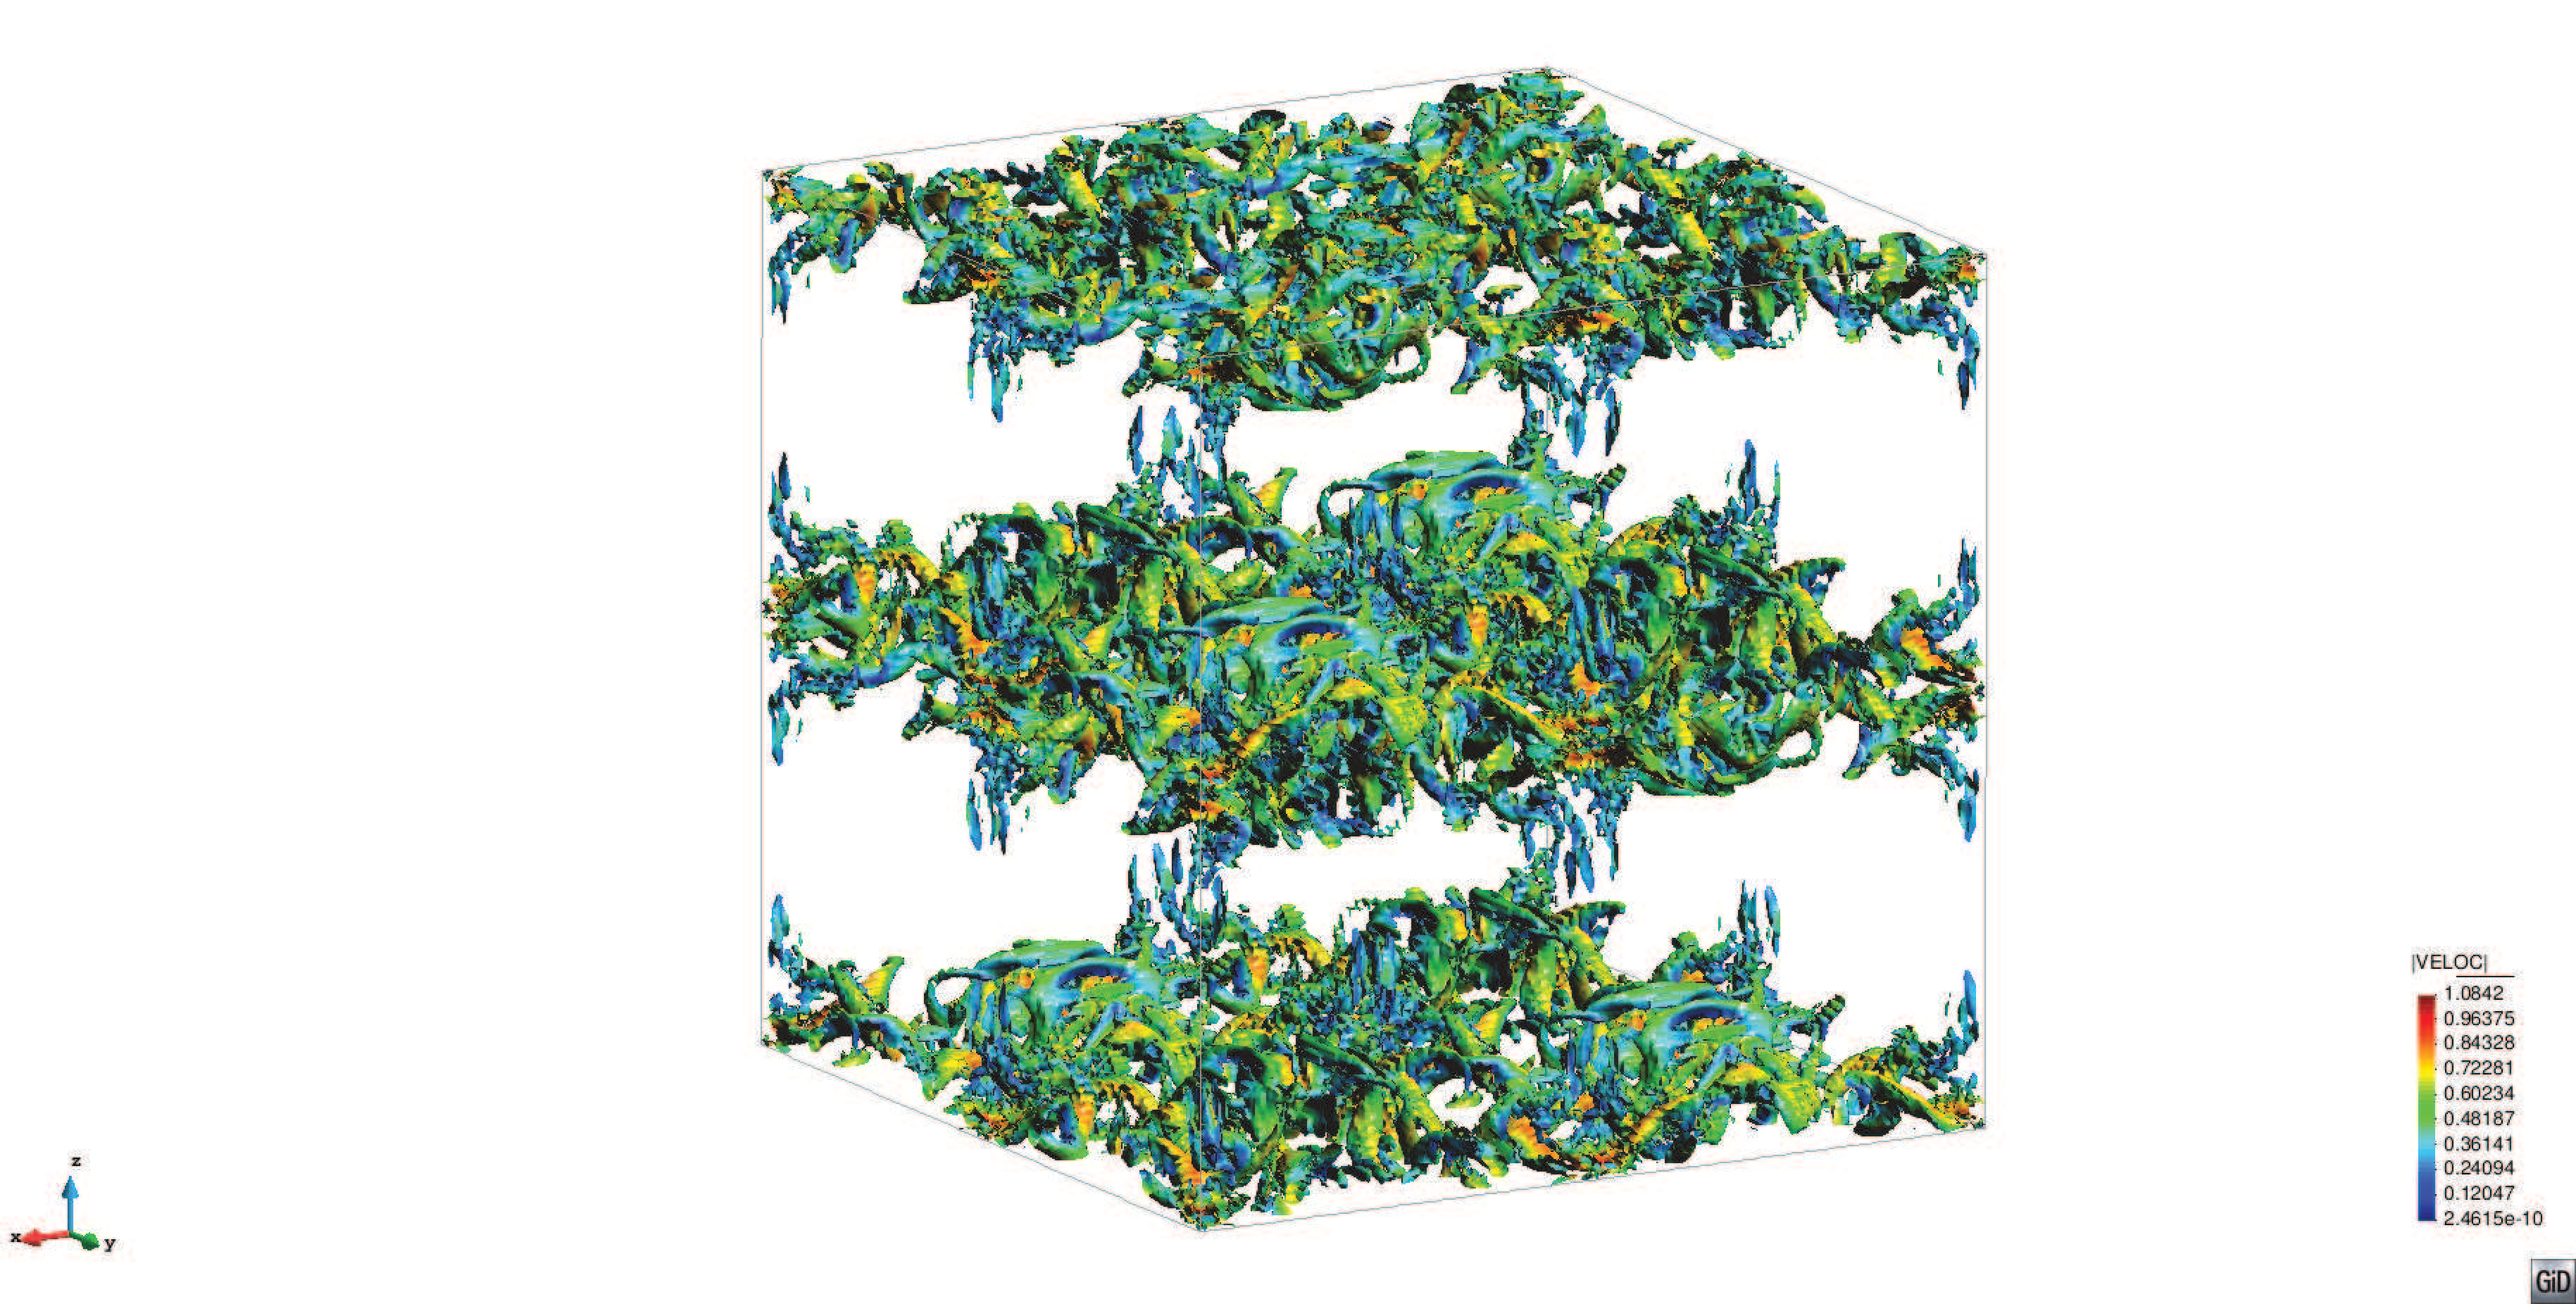
\includegraphics[width=1.0\textwidth]{Figures/isovorti_veloc_6}}{Movies/TGV.flv}
  \caption{Velocity isosurface}
\end{figure}}
\end{frame}
%---------------------------------------------------------------------------
\begin{frame}[t]
\frametitle{TCF {\small Turbulent Channel Flow}}
\textbf{Mean streamwise velocity (models):}
 \vspace*{-0.3cm}
  \begin{figure}
    \centering	
    \only<1-3>{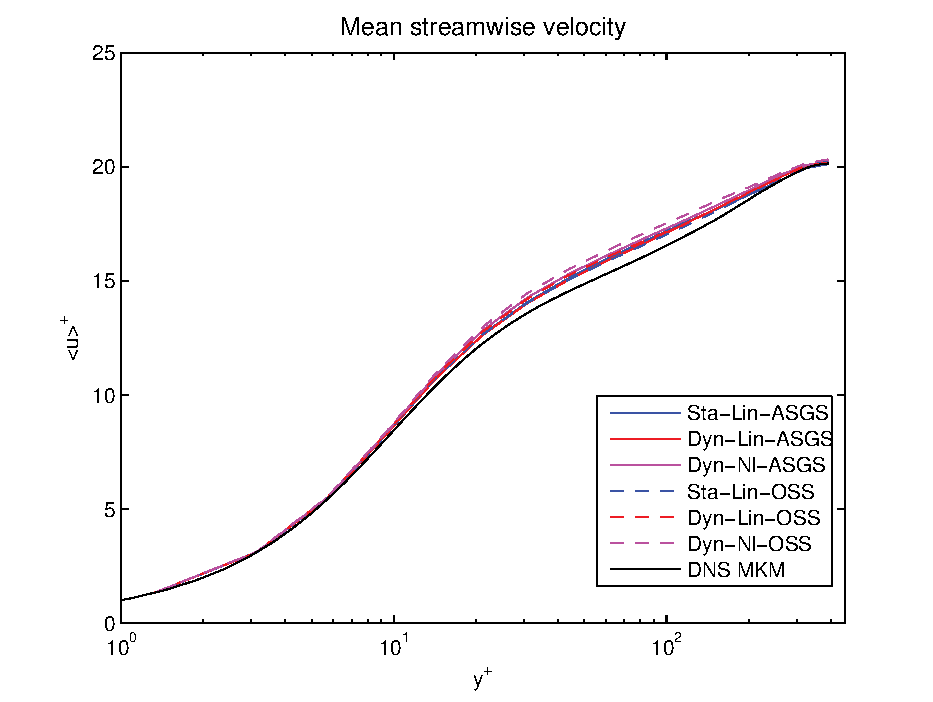
\includegraphics[width=0.65\textwidth]{Figures/Rb_TCF/umean}}
    \only<4>{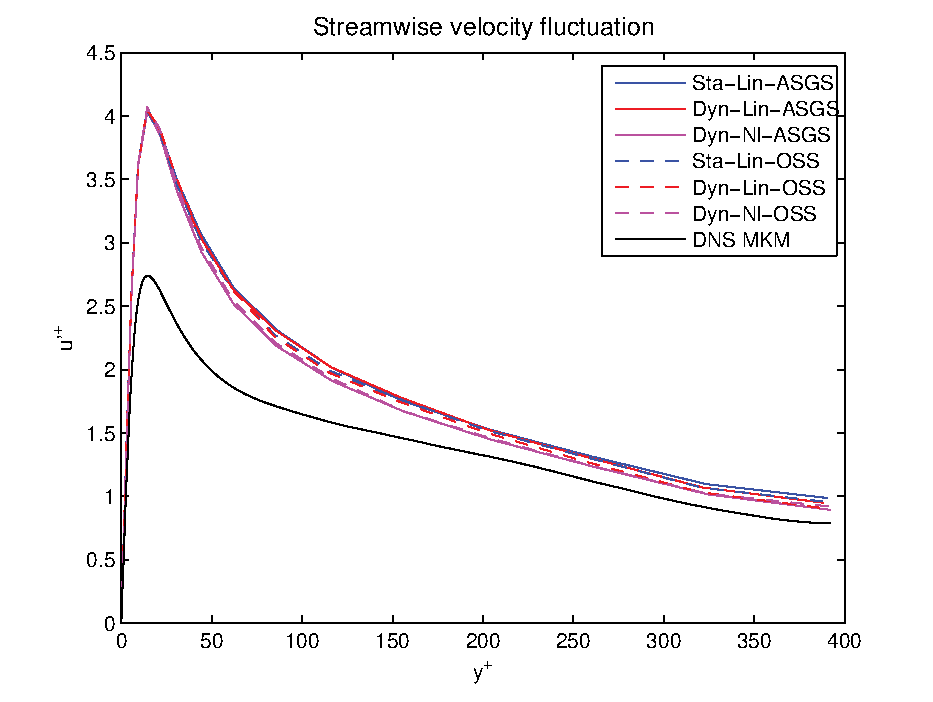
\includegraphics[width=0.65\textwidth]{Figures/Rb_TCF/ufluc}}
    \only<5>{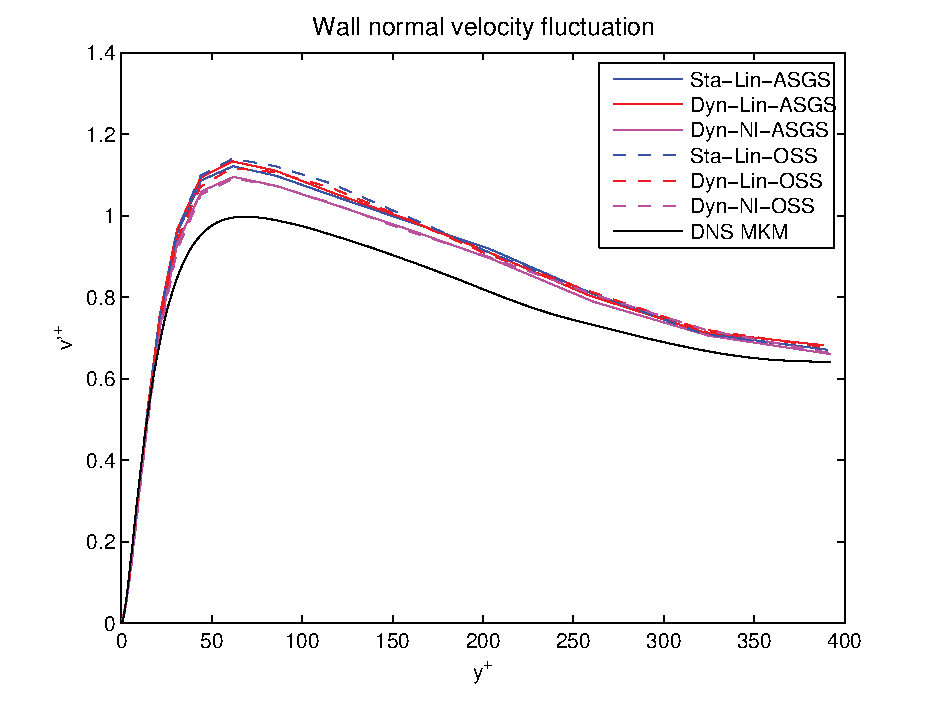
\includegraphics[width=0.65\textwidth]{Figures/Rb_TCF/vfluc}}
    \only<6>{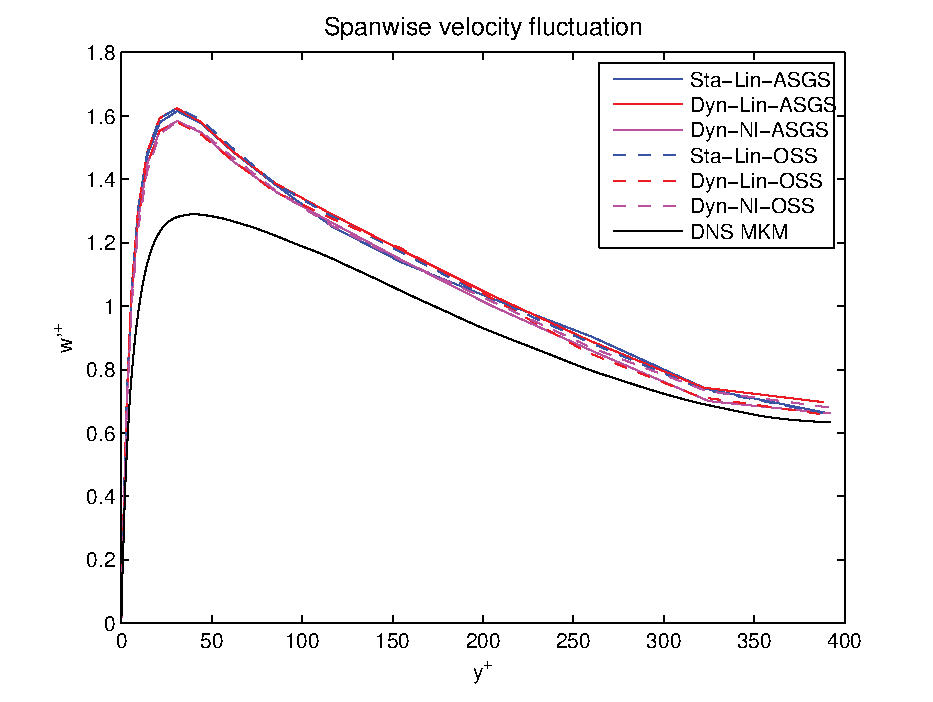
\includegraphics[width=0.65\textwidth]{Figures/Rb_TCF/wfluc}} 
  \end{figure}
  \vspace*{-0.5cm}
   \begin{overlayarea}{\textwidth}{1.5cm}
 \only<2->{
 \begin{itemize}
  	\item \alert<2>{Small differences between methods}
  	\only<3->{\item Very \alert<3>{accurate results} compared against the \alert<3>{DNS}}
  \end{itemize}}
  \end{overlayarea}
\end{frame}

%=========================================================================================
% 2.4.CONCLUSIONS
% ----------------------------------------------------------------------------
\subsection{Conclusions}
%----------------------------------------------------------------------------------------
\begin{frame}
\frametitle{RB-VMS Conclusions}
\vfill
\begin{itemize}
	\onslide<1->{\item VMS formulations of NS equations can be used for the numerical simulation of turbulent flows.}
	\onslide<2->{\item Our particular VMS modelling ingredients
  	\begin{itemize}
  		\item Dynamic subscales
  		\item Nonlinear subscales
  		\item Orthgonal subscales
  	\end{itemize}
	seem to be important to reduce the computational cost.}
	%(semidicrete stability, convergence to weak solutions).
	\onslide<3->{\item Among them dynamic and orthogonal subscales (linear or nonlinear) are the most effective.}
	\onslide<4->{\item The skewsymmetric formulation is important to keep stability.}
	%\item Further numerical examples are being carried out (Taylor Green, Channel flow).
\end{itemize}
\vfill
\end{frame}
%----------------------------------------------------------------------------------------
\begin{frame}
\frametitle{RB-VMS Limitations}
\vfill
\begin{itemize}
	\item<1-> \textbf{ASGS:}
	\begin{itemize}
		\item<2-> Poorly matrix conditioning $ \Rightarrow $ \alert{High} number of \alert{solver} iterations.
		\item<3-> No explicit projections $ \Rightarrow $ \algreen{3-}{Low} number of \algreen{3-}{nonlinear} iterations.
	\end{itemize}
	\item<4-> \textbf{OSS:}
	\begin{itemize}
		\item<5-> Better matrix conditioning $ \Rightarrow $ \algreen{5-}{Low} number of \algreen{5-}{solver} iterations.
		\item<6-> Explicit projection treatment $ \Rightarrow $ \alert{High} number of \alert{nonlinear} iterations.
	\end{itemize}
	\item<7-> \textbf{Desired:} 
		\begin{itemize}
		\item<7-> OSS with implicit projections.
		\end{itemize}
\end{itemize}
\vfill
\end{frame}


%=========================================================================================
% 3.MIXED FE VMS
% ----------------------------------------------------------------------------
\section{Mixed FE VMS}
\addtocounter{framenumber}{-1}
\frame{
\begin{minipage}[\textheight]{0.5\textwidth}
\vfill
\tableofcontents[currentsection,
				subsubsectionstyle=hide,
				sectionstyle=show/shaded, 
				subsectionstyle=show/show/hide]
\vfill
\end{minipage}
\begin{minipage}[\textheight]{0.4\textwidth}
  	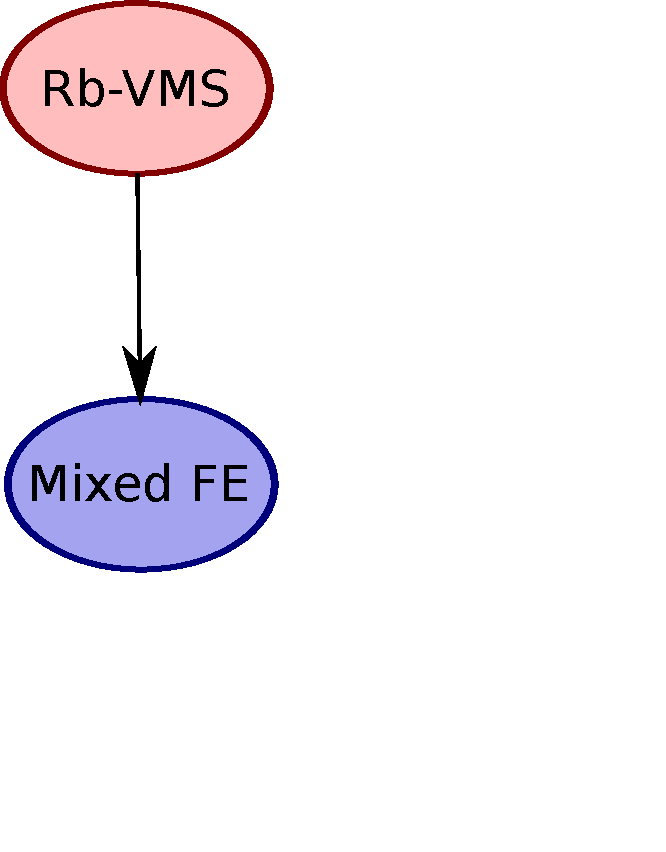
\includegraphics[width=1.1\textwidth]{Figures/index_2}
\end{minipage}
}
\begin{frame}
\frametitle{Motivation}
\vfill
\textbf{Step by step...}
\begin{itemize}
\item \algreen{1}{Residual-based VMS as LES models}
\alert<1>{\item Mixed FE formulations as LES models}
\item High-order time integration schemes
\item Velocity-pressure segregation
\item Scalable solvers
\end{itemize}
\vfill
\end{frame}

%=========================================================================================
% 3.1.FORMULATION
% ----------------------------------------------------------------------------
\subsection{Formulation}
\begin{frame}[t]
\frametitle{Semidiscrete problem}
\begin{block}{FEM equations}
\begin{overlayarea}{\textwidth}{2.0cm}
\vspace{-0.8cm}
\begin{align*}
% FEM EQUATIONS
\left( \mathbf{v}_{h},\partial _{t}\mathbf{u}_{h}\right) _{\Omega }
+ b\left(\mathbf{a},\mathbf{u}_h, \mathbf{v}_h\right)
+\left( \mathbf{\nabla v}_{h},\nu \mathbf{\nabla u}_{h}\right) _{\Omega} &
-\left( \mathbf{\nabla }\cdot \mathbf{v}_{h},p_{h}\right) _{\Omega }
\\[0.05in]
\onslide<1>{+\left( \mathbf{v}_{h},\partial _{t}\widetilde{\mathbf{u}}\right) _{\Omega}}
\alert<2->{+\left( \mathcal{L}^{\ast }\mathbf{v}_{h},\widetilde{\mathbf{u}}\right)_{\Omega^h}
-\left( \mathbf{\nabla }\cdot \mathbf{v}_{h},\widetilde{p}\right) _{\Omega^h}} &
=\left\langle \mathbf{v}_{h},\mathbf{f}\right\rangle_{\Omega }
\\[0.1in]
\left( q_{h},\mathbf{\nabla }\cdot \mathbf{u}_{h}\right) _{\Omega }
\alert<2->{-\left( \mathbf{\nabla }q_{h},\widetilde{\mathbf{u}}\right) _{\Omega^h}} & =0
\end{align*}
\end{overlayarea}
\end{block}
\begin{block}{SGS equations}
\vspace{-0.4cm}
\begin{align*}
% SGS EQUATIONS
\onslide<1>{\partial_{t}\widetilde{\mathbf{u}} +} \alert<2->{\tau_{m}^{-1} \widetilde{\mathbf{u}}}
&= \alert<2->{\mathcal{P} \mathbf{R}_{m}}
\\[0.05in]
%\\[0.1in]
\tau _{c}^{-1} \widetilde{p} & = \mathcal{P} R_{c}
\end{align*}
\end{block}
%\end{overlayarea}
\vspace{-0.2cm}
\begin{overlayarea}{\textwidth}{3.0cm}
\begin{equation*}
\onslide<1>{\mathcal{P} = I \quad \rm{(ASGS)},} \quad \quad \alert<2->{\mathcal{P} = P_h^{\perp}=I-P_h \quad \rm{(OSS)}}
\end{equation*}
\vspace{-0.2cm}
\begin{equation*}
\alert<2->{\mathbf{a=u}_{h}}\onslide<1>{+\widetilde{\mathbf{u}}}
\end{equation*}
\end{overlayarea}
\end{frame}
%----------------------------------------------------------------------------------------
\begin{frame}[t]
\frametitle{Term-by-term OSS}
\only<1>{
\begin{block}{FEM equations}
\begin{overlayarea}{\textwidth}{6.0cm}
\vspace{-0.8cm}
\begin{align*}
% FEM EQUATIONS
\left( \mathbf{v}_{h},\partial _{t}\mathbf{u}_{h}\right) _{\Omega }
+ b\left(\mathbf{a},\mathbf{u}_h, \mathbf{v}_h\right)
+\left( \mathbf{\nabla v}_{h},\nu \mathbf{\nabla u}_{h}\right) _{\Omega} &
-\left( \mathbf{\nabla }\cdot \mathbf{v}_{h},p_{h}\right) _{\Omega }
\\[0.05in]
\onslide<0>{+\left( \mathbf{v}_{h},\partial _{t}\widetilde{\mathbf{u}}\right) _{\Omega}}
\alert<1->{+\left( \mathcal{L}^{\ast }\mathbf{v}_{h},\widetilde{\mathbf{u}}\right)_{\Omega^h}
-\left( \mathbf{\nabla }\cdot \mathbf{v}_{h},\widetilde{p}\right) _{\Omega^h}} &
=\left\langle \mathbf{v}_{h},\mathbf{f}\right\rangle_{\Omega }
\\[0.1in]
\left( q_{h},\mathbf{\nabla }\cdot \mathbf{u}_{h}\right) _{\Omega }
\alert<1->{-\left( \mathbf{\nabla }q_{h},\widetilde{\mathbf{u}}\right) _{\Omega^h}} & =0
\end{align*}
\end{overlayarea}
\end{block}}
\only<2->{
\begin{block}{Term-by-term OSS (Codina 2008)}
\begin{overlayarea}{\textwidth}{6.0cm}
\vspace{-0.8cm}
\begin{align*}
&\left( \mathbf{v}_{h},\partial _{t}\mathbf{u}_{h}\right) _{\Omega }
+ b\left(\mathbf{a},\mathbf{u}_h, \mathbf{v}_h\right)
+\left( \mathbf{\nabla v}_{h},\nu \mathbf{\nabla u}_{h}\right) _{\Omega} 
-\left( \mathbf{\nabla }\cdot \mathbf{v}_{h},p_{h}\right) _{\Omega }
\\[0.05in]
&+\only<2>{\alert<2>{\left(\tau_m \mathbf{a}\cdot\nabla\mathbf{v}_{h},\mathcal{P}_h^\perp(\mathbf{a}\cdot\nabla\mathbf{u}_{h})\right)_{\Omega^h}}}
\only<3>{\alert<3>{\left(\tau_m \mathbf{a}\cdot\nabla\mathbf{v}_{h},\mathbf{a}\cdot\nabla\mathbf{u}_{h}\right)_{\Omega^h}-\left(\tau_m \mathbf{a}\cdot\nabla\mathbf{v}_{h},\boldsymbol{\eta}_{h}\right)_{\Omega^h}}}\\
&+\only<2>{\alert<2>{\left(\tau_c \nabla\cdot\mathbf{v}_{h},\mathcal{P}_h^\perp(\nabla\cdot\mathbf{u}_{h})\right) _{\Omega^h}} }
\only<3>{\alert<3>{\left(\tau_c \nabla\cdot\mathbf{v}_{h},\nabla\cdot\mathbf{u}_{h}\right) _{\Omega^h}} }
=\left\langle \mathbf{v}_{h},\mathbf{f}\right\rangle_{\Omega }
\\[0.1in]
%
&\left( q_{h},\mathbf{\nabla }\cdot \mathbf{u}_{h}\right) _{\Omega }
+\only<2>{\alert<2>{\left(\tau_m \nabla q_{h},\mathcal{P}_h^\perp(\nabla p_{h})\right) _{\Omega^h}} }
\only<3>{\alert<3>{\left(\tau_m \nabla q_{h},\nabla p_{h}\right) _{\Omega^h}-\left(\tau_m \nabla q_{h},\boldsymbol{\xi}_{h}\right) _{\Omega^h}}}
 =0
\end{align*}
\only<3->{
\begin{align*}
&\boldsymbol{\eta}_{h}:=\mathcal{P}_h(\mathbf{a}\cdot\nabla\mathbf{u}_{h})\\
&\boldsymbol{\xi}_{h}:=\mathcal{P}_h(\nabla p_{h})\\
&\mathcal{P}_h(\nabla\cdot\mathbf{u}_{h})\approx 0
\end{align*}}
\end{overlayarea}
\end{block}}
\end{frame}
%----------------------------------------------------------------------------------------
\begin{frame}
\frametitle{Matricial form}
%\begin{overlayarea}{\textwidth}{6.0cm}
\begin{itemize}
\item<1-> ASGS:
\begin{equation*}
\left[\begin{array}{c}
\M\dot{\U}\\
\mathbf{0}
\end{array}\right]+\left[\begin{array}{cc}
K+C+A_\tau&G\\
D&L_\tau
\end{array}\right]\left[\begin{array}{c}
\U\\
\P
\end{array}\right]=\left[\begin{array}{c}
\F_u\\
\mathbf{0}
\end{array}\right],
\end{equation*}
\item<2-> Term-by-term OSS:
\begin{equation*}
\left[\begin{array}{c}
M\dot{\U}\\
\mathbf{0}\\
\mathbf{0}\\
\mathbf{0}
\end{array}\right]+\left[\begin{array}{cccc}
K+C+A_\tau&G&B_{\eta,\tau}&0\\
D&L_\tau&0&B_{\xi,\tau}\\
B_{\eta,\tau}^T&0&M_{\eta,\tau}&0\\
0&B_{\xi,\tau}^T&0&M_{\xi,\tau}
\end{array}\right]\left[\begin{array}{c}
\U\\
\P\\
\ETA\\
\XI
\end{array}\right]=\left[\begin{array}{c}
\F_u\\
\mathbf{0}\\
\mathbf{0}\\
\mathbf{0}
\end{array}\right],
\end{equation*}
\item<3-> Term-by-term OSS with Inf-sup stable elements (mixed FE):
\begin{equation*}
\left[\begin{array}{c}
M\dot{\U}\\
\mathbf{0}\\
\mathbf{0}
\end{array}\right]+\left[\begin{array}{ccc}
K+C+A_\tau&G&B_\tau\\
D&0&0\\
B_\tau^T&0&M_\tau
\end{array}\right]\left[\begin{array}{c}
\U\\
\P\\
\ETA
\end{array}\right]=\left[\begin{array}{c}
\F_u\\
\mathbf{0}\\
\mathbf{0}
\end{array}\right],
\end{equation*}
\end{itemize}
%\end{overlayarea}
\end{frame}
%%----------------------------------------------------------------------------------------
%\begin{frame}
% \frametitle{TGV {\small Taylor-Green Vortex flow}}
% \textbf{Energy dissipation rate (different methods):}
% \begin{itemize}
% 	\itemsep-0.1cm
%  	\item Different mesh discretizations for ASGS and OSS ($ Q_1/Q_1 $,$ Q_2/Q_2 $)
%  	\item $ Q_2/Q_1 $ discretization for mixed FE OSS.
% \end{itemize}
% \vspace*{-0.5cm}
% \begin{figure}
%     \centering	
%     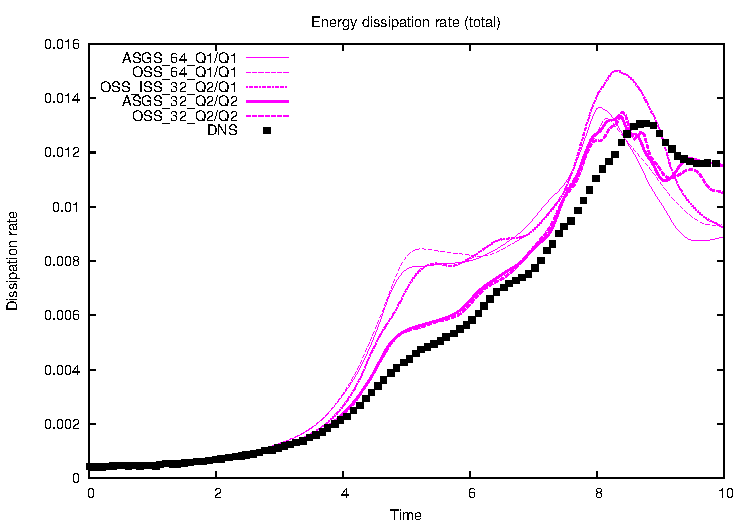
\includegraphics[width=0.6\textwidth]{Figures/oss_64_tot.pdf}
%     \vspace*{-0.2cm}
% \end{figure}
% \begin{overlayarea}{\textwidth}{1.5cm}
% \only<2->{
% \vspace*{-0.5cm}
% \begin{itemize}
% 	\itemsep-0.1cm
%  	\item \alert<2>{Good agreement with the DNS} (coarse mesh).
%  	\only<3->{\item \alert<3>{More accurate results with equal-order elements}.}
%  \end{itemize}}
%  \end{overlayarea}
%\end{frame}
%%----------------------------------------------------------------------------------------
%\begin{frame}
% \frametitle{TGV {\small Taylor-Green Vortex flow}}
% \textbf{Computational cost (different methods):}
% \begin{itemize}
% 	\itemsep-0.1cm
%  	\item Acumulated solver iterations.
% \end{itemize}
% \vspace*{-0.5cm}
% \begin{figure}
%     \centering	
%     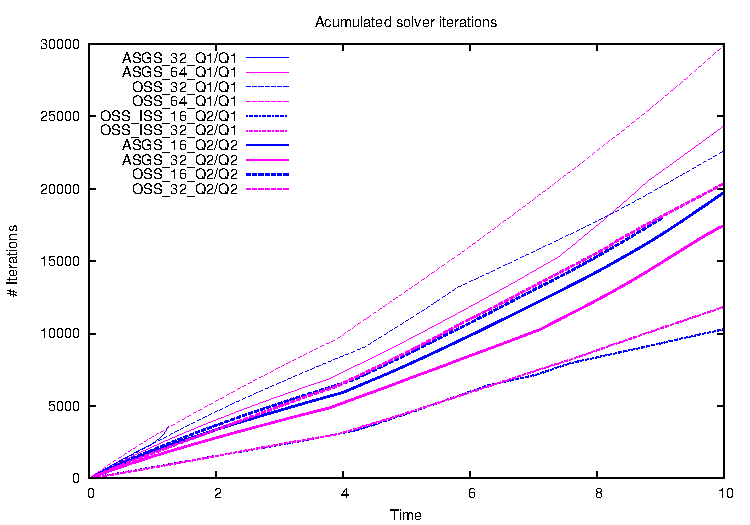
\includegraphics[width=0.7\textwidth]{Figures/oss_all_acu.pdf}
%     \vspace*{-0.2cm}
% \end{figure}
% \begin{overlayarea}{\textwidth}{1.5cm}
% \only<2->{
% \vspace*{-0.5cm}
% \begin{itemize}
% 	\itemsep-0.1cm
%  	\item \alert<2>{Mixed FE OSS cheapest}.
%  \end{itemize}}
%  \end{overlayarea}
%\end{frame}
%%----------------------------------------------------------------------------------------
%\begin{frame}
%\frametitle{Mixed FE OSS Conclusions}
%\begin{itemize}
%\item<1-> Better results for equal-order interpolations.
%\item<2-> Mixed FE OSS the cheapest method.
%\item<3-> Mixed FE OSS $ Q_2/Q_1 $ better and cheaper than other methods with $ Q_1/Q_1 $. 
%\end{itemize}
%\end{frame}

%=========================================================================================
% 3.2.BLOCK-PRECONDITIONING
% ----------------------------------------------------------------------------
\subsection{Block-preconditioning}
\begin{frame}
\frametitle{Block-recursive preconditioning}
%\begin{overlayarea}{\textwidth}{6.0cm}
\vspace{-0.3cm}
General case:
\only<1>{
\begin{equation*}
\left[\begin{array}{c}
M\dot{\U}\\
\mathbf{0}\\
\mathbf{0}\\
\mathbf{0}
\end{array}\right]+\left[\begin{array}{cccc}
K+C+A_\tau&G&B_{\eta,\tau}&0\\
D&L_\tau&0&B_{\xi,\tau}\\
-B_{\eta,\tau}^T&0&M_{\eta,\tau}&0\\
0&-B_{\xi,\tau}^T&0&M_{\xi,\tau}
\end{array}\right]\left[\begin{array}{c}
\U\\
\P\\
\ETA\\
\XI
\end{array}\right]=\left[\begin{array}{c}
\F_u\\
\mathbf{G}\\
\mathbf{0}\\
\mathbf{0}
\end{array}\right],
\end{equation*}}
\only<2-8>{
\begin{equation*}
\left[\begin{array}{c}
M\dot{\U}\\
\mathbf{0}\\\hdashline
\mathbf{0}\\
\mathbf{0}
\end{array}\right]+\left[\begin{array}{cc:cc}
K+C+A_\tau&G&B_{\eta,\tau}&0\\
D&L_\tau&0&B_{\xi,\tau}\\\hdashline
-B_{\eta,\tau}^T&0&M_{\eta,\tau}&0\\
0&-B_{\xi,\tau}^T&0&M_{\xi,\tau}
\end{array}\right]\left[\begin{array}{c}
\U\\
\P\\\hdashline
\ETA\\
\XI
\end{array}\right]=\left[\begin{array}{c}
\F_u\\
\mathbf{G}\\\hdashline
\mathbf{0}\\
\mathbf{0}
\end{array}\right],
\end{equation*}}
\only<9->{
\begin{equation*}
\left[\begin{array}{c}
M\dot{\U}\\
\mathbf{0}\\\hdashline
\mathbf{0}\\
\mathbf{0}
\end{array}\right]+\left[\begin{array}{cc:cc}
\multicolumn{1}{c|}{K+C+A_\tau}&G&B_{\eta,\tau}&0\\
\cline{1-2}
\multicolumn{1}{c|}{D}&L_\tau&0&B_{\xi,\tau}\\\hdashline
-B_{\eta,\tau}^T&0&M_{\eta,\tau}&0\\
0&-B_{\xi,\tau}^T&0&M_{\xi,\tau}
\end{array}\right]\left[\begin{array}{c}
\U\\
\P\\\hdashline
\ETA\\
\XI
\end{array}\right]=\left[\begin{array}{c}
\F_u\\
\mathbf{G}\\\hdashline
\mathbf{0}\\
\mathbf{0}
\end{array}\right],
\end{equation*}}
\vspace{-0.5cm}
\only<3->{
\begin{itemize}
\only<3-8>{\item Outer block matrix:}
\only<3>{
\begin{equation*}
\widetilde{A}=\left[\begin{array}{cc:cc}
M_{\eta,\tau}&0&-B_{\eta,\tau}^T&0\\
0&M_{\xi,\tau}&0&-B_{\xi,\tau}^T\\\hdashline
B_{\eta,\tau}&0&K+C+A_\tau&G\\
0&B_{\xi,\tau}&D&L_\tau
\end{array}\right]
\end{equation*}}
\only<4-8>{
\begin{align*}
\onslide<5->{
\widetilde{A}&=\left[\begin{array}{cc}
\widetilde{M}_{\tau}&-\widetilde{B}_{\tau}^T\\
\widetilde{B}_{\tau}&\widetilde{K}_\tau
\end{array}\right]=\left[\begin{array}{cc}
I&0\\
\widetilde{B}_{\tau}{\widetilde{M}_{\tau}}^{-1}&I
\end{array}\right]\left[\begin{array}{cc}
\widetilde{M}_{\tau}&-\widetilde{B}_{\tau}^T\\
0&\widetilde{S}
\end{array}\right],}\\
\onslide<6->{
\widetilde{S}&=\widetilde{K}_\tau+\widetilde{B}_{\tau}{\widetilde{M}_{\tau}}^{-1}\widetilde{B}_{\tau}^T,}\\
\onslide<7->{
P_U(\widetilde{A})&=\left[\begin{array}{cc}
\widetilde{M}_{\tau}&-\widetilde{B}_{\tau}^T\\
0&\widetilde{S}
\end{array}\right]^{-1}=\left[\begin{array}{cc}
\widetilde{M}_{\tau}^{-1}&\widetilde{M}_{\tau}^{-1}\widetilde{B}_{\tau}^T\widetilde{S}^{-1}\\
0&\widetilde{S}^{-1}
\end{array}\right],}\\ 
\onslide<8->{
\widetilde{S}^{-1}&\approx\widetilde{K}_\tau^{-1}.}
\end{align*}}
\only<9-12>{\item Inner block matrix:}
\only<9->{
\begin{align*}
\onslide<9->{
\widetilde{K}_\tau&=\left[\begin{array}{cc}
K_\tau&G\\
D&L_\tau
\end{array}\right]=\left[\begin{array}{cc}
I&0\\
DK_\tau^{-1}&I
\end{array}\right]\left[\begin{array}{cc}
K_\tau&G\\
0&S
\end{array}\right],}\\
\onslide<10->{
S&=L_\tau-DK_\tau^{-1} G,}\\
\onslide<11->{
P_U(\widetilde{K}_\tau)&=\left[\begin{array}{cc}
K_\tau&G\\
0&S
\end{array}\right]^{-1}=\left[\begin{array}{cc}
K_\tau^{-1}&-K_\tau^{-1}GS^{-1}\\
0&S^{-1}
\end{array}\right],}\\ 
\onslide<12->{
\widetilde{S}^{-1}&\approx L_p^{-1}.}
\end{align*}}
\end{itemize}}
%\end{overlayarea}
\end{frame}
%%----------------------------------------------------------------------------------------


%=========================================================================================
% 3.3.NUMERICAL EXPERIMENTS
% ----------------------------------------------------------------------------
\subsection{Numerical experiments}
\begin{frame}[t]
\frametitle{Numerical experiments}
\vfill
Manufactured analytical solution:
\begin{itemize}
\item Colliding flow.
\end{itemize}
\vspace{1cm}
Two different turbulent benchmarks:
\begin{itemize}
\item Taylor-Green Vortex (TGV) flow.
\item Turbulent Channel Flow (TCF).
\end{itemize}
\vfill
\end{frame}

%=========================================================================================
% 3.3.1.COLLIDING FLOW
% ----------------------------------------------------------------------------
\subsubsection{Analytical colliding flow}
%----------------------------------------------------------------------------------------
\begin{frame}
  \frametitle{Colliding flow}
  \textbf{Problem setting:}
  \begin{itemize}
    \itemsep-0.10cm
 	\item Analytical solution
  	\item $Re=25$ 
  	\item Mesh refinement: $ 4^3 $ to $ 64^3 $ $ Q1/Q1 $ elements (ASGS and OSS) or $ 2^3 $ to $ 32^3 $$ Q2/Q1 $ elements (OSS-ISS)
  \end{itemize}
  \vspace*{-0.3cm}
  \begin{figure}
    \centering	
    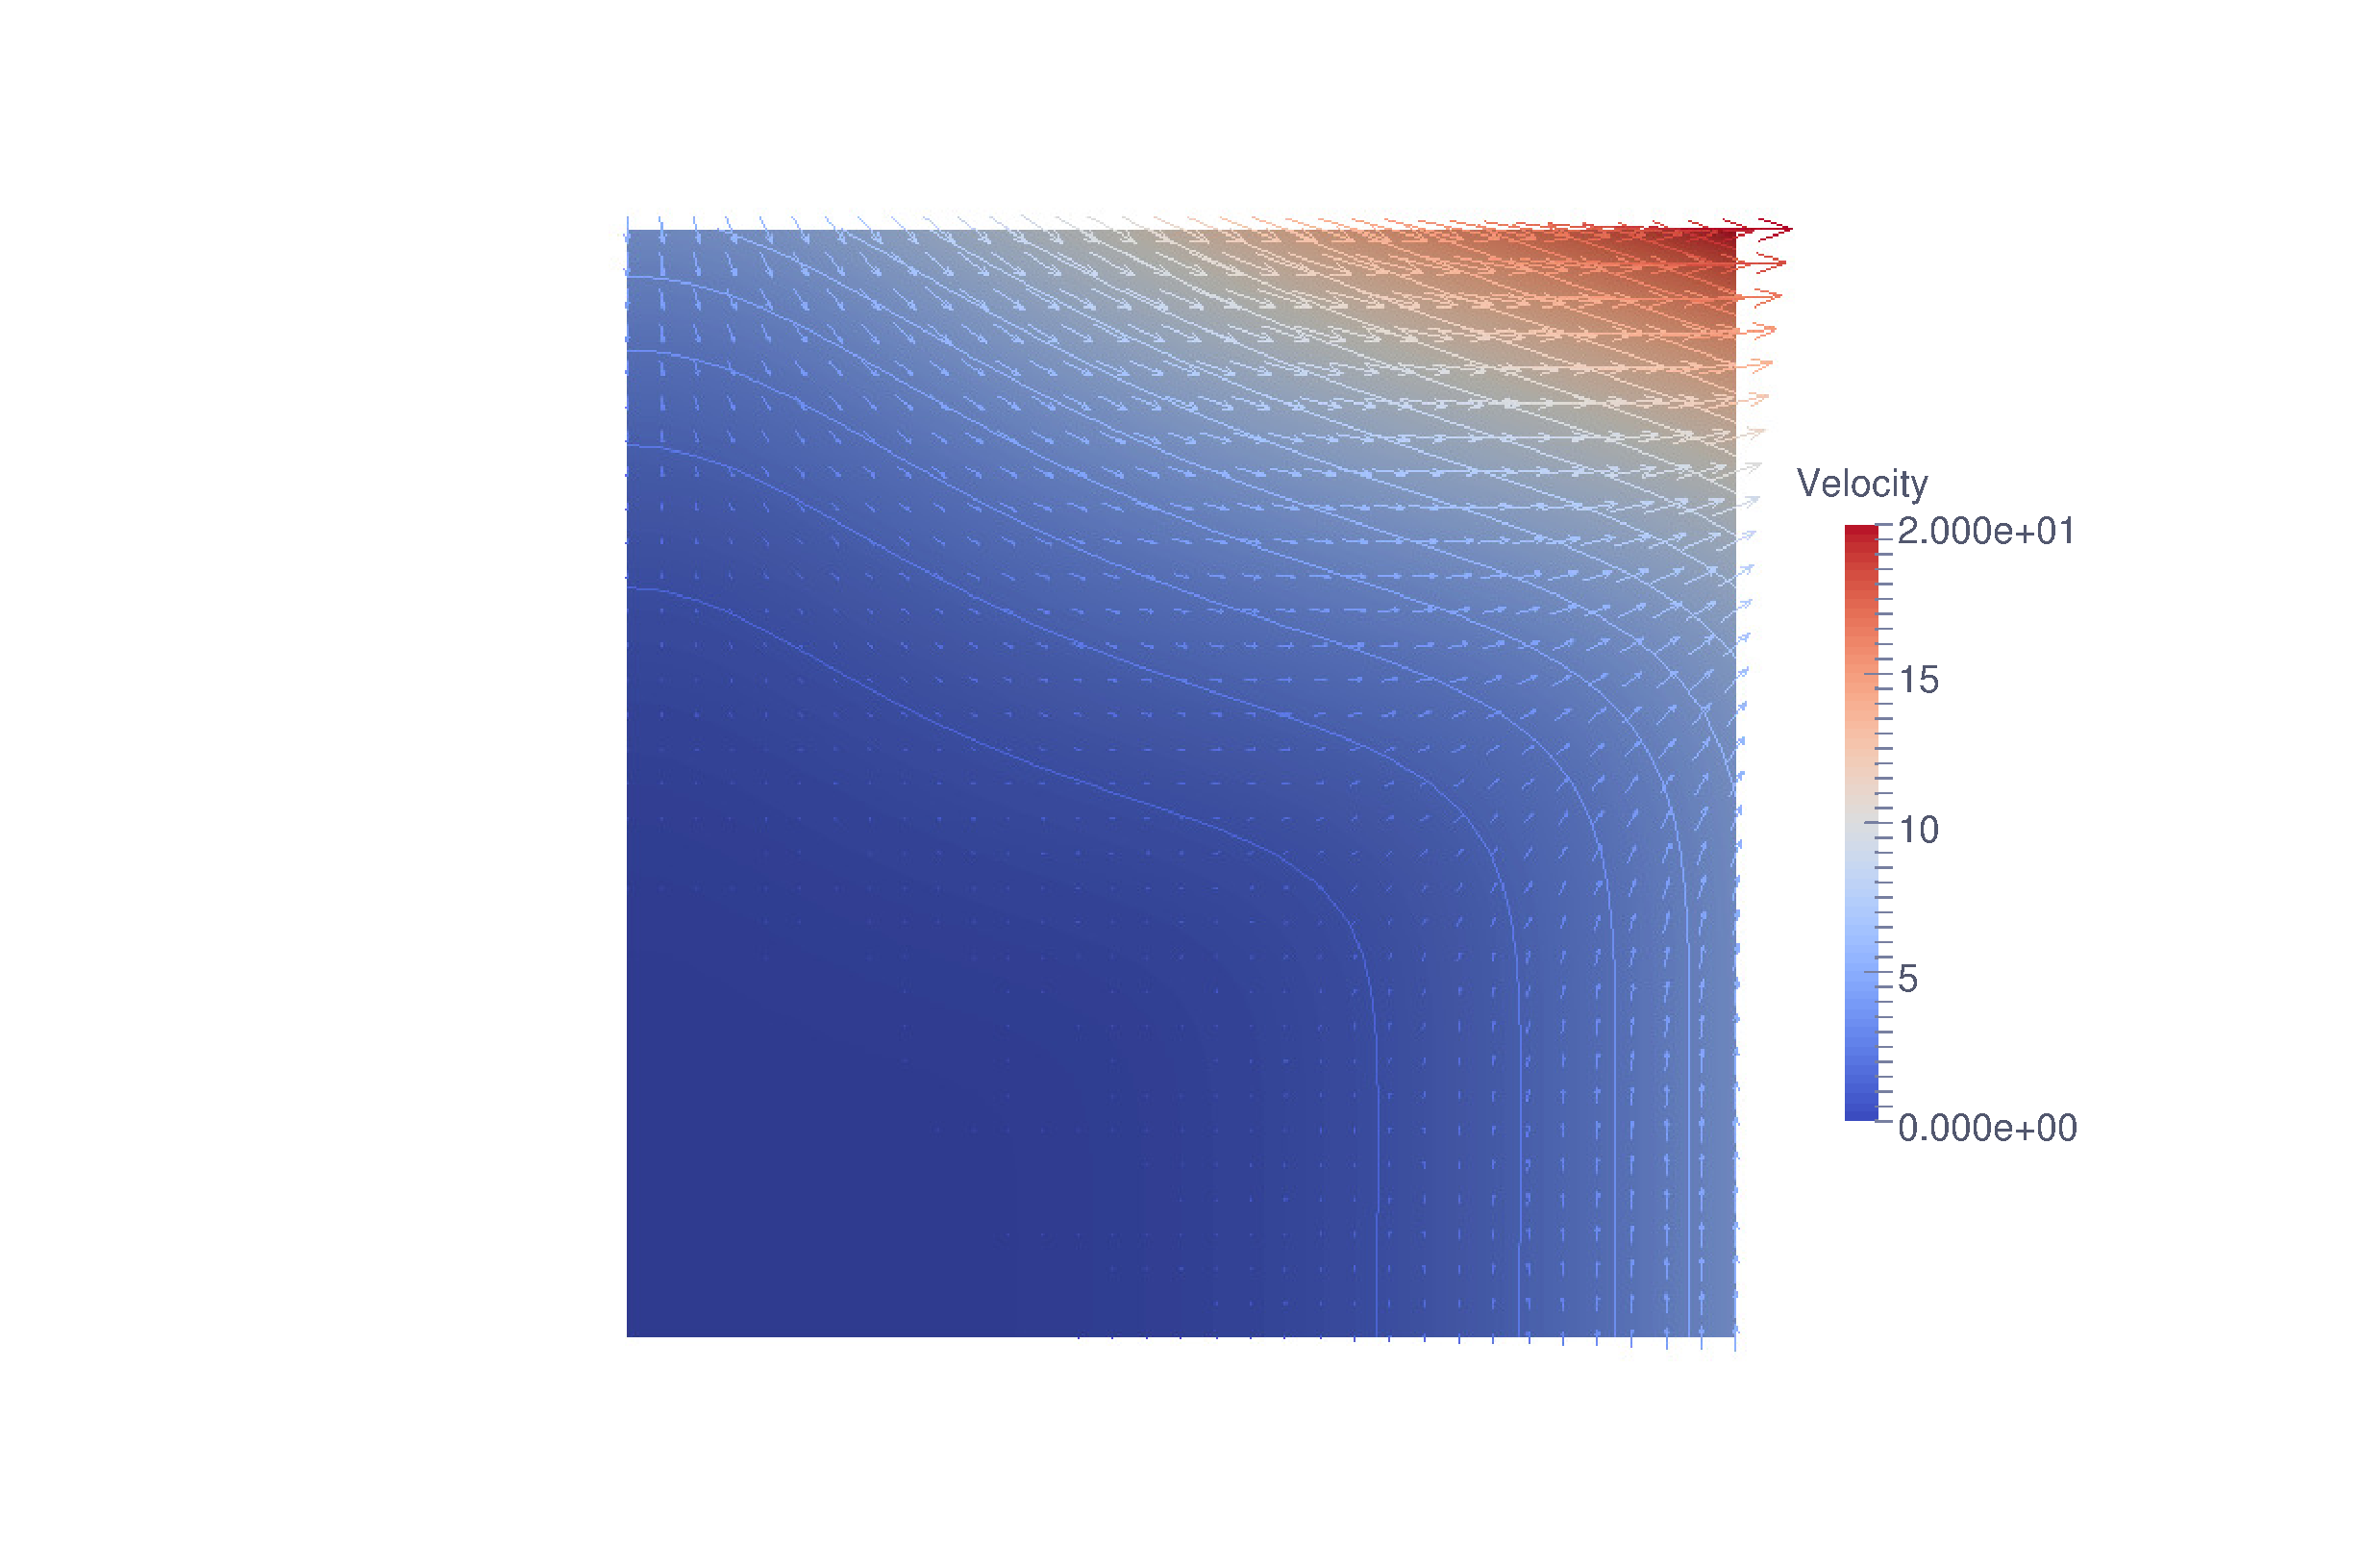
\includegraphics[trim=10cm 3.5cm 5cm 3cm, clip=true, width=0.5\textwidth]{Figures/colliding_flow.pdf}
	\vspace*{-0.2cm}
	\caption{Velocity field}
  \end{figure}
\end{frame}
%----------------------------------------------------------------------------------------
\begin{frame}
 \frametitle{Colliding flow}
 \textbf{Accumulated solver iterations:} (using $ P_U(\widetilde{A}) $)
  \vspace*{-0.25cm}
 \begin{figure}
     \centering	
     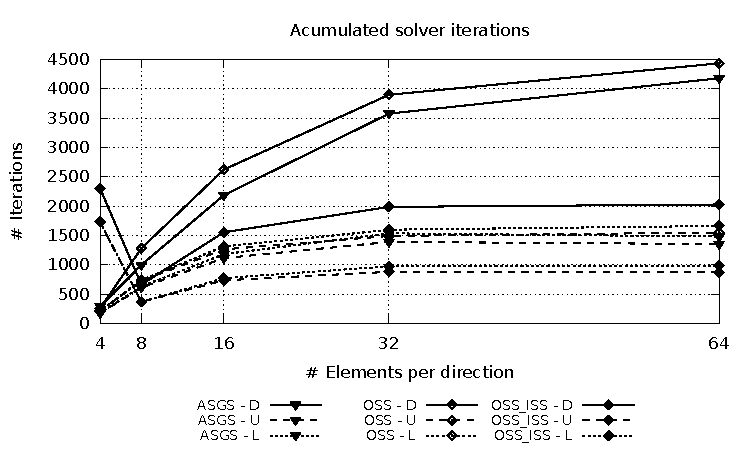
\includegraphics[width=0.8\textwidth]{Figures/colliding_iter.pdf}
   \end{figure}
 \begin{overlayarea}{\textwidth}{1.5cm}
 \only<2->{
 \vspace*{-0.6cm}
 \begin{itemize}
  	\item \alert<2>{$ P_U(\widetilde{K}_\tau) $ and $ P_L(\widetilde{K}_\tau) $ optimal block-preconditioners} for all methods
  	\only<3->{\item \alert<3>{Less solver iterations for the OSS-ISS method} with the same velocity DOFs}
  \end{itemize}}
  \end{overlayarea}
\end{frame}
%----------------------------------------------------------------------------------------
\begin{frame}
 \frametitle{Colliding flow}
 \textbf{Efficiency:} \only<1-2>{Velocity}\only<3>{Pressure}
   \vspace*{-0.25cm}
 \only<1-2>{
 \begin{figure}
     \centering	
     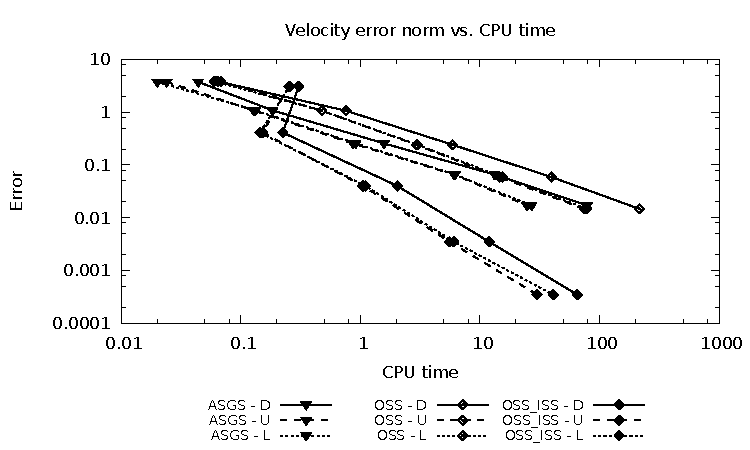
\includegraphics[width=0.8\textwidth]{Figures/colliding_errtu.pdf}
   \end{figure}}
\only<3->{
\begin{figure}
    \centering	
    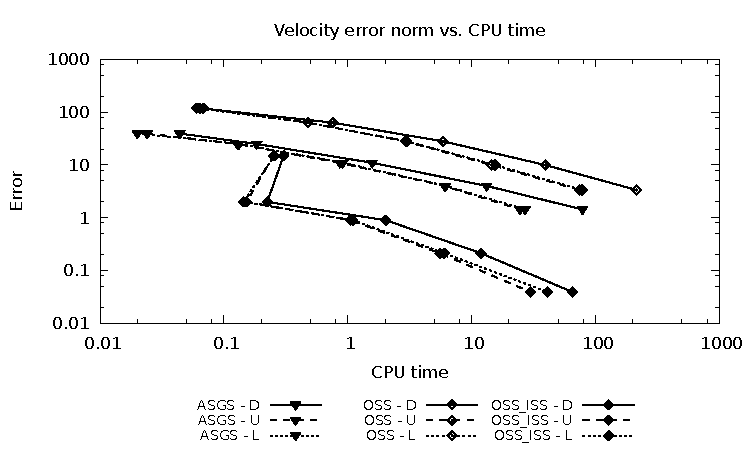
\includegraphics[width=0.8\textwidth]{Figures/colliding_errtp.pdf}
  \end{figure}}
 \begin{overlayarea}{\textwidth}{1.5cm}
  \vspace*{-0.5cm}
 \only<2>{
 \begin{itemize}
  	\item \alert<2>{OSS-ISS the most efficient method}
  \end{itemize}}
   \only<3->{
   \begin{itemize}
    	\item \alert<3>{Also for pressures}
    \end{itemize}}
  \end{overlayarea}
\end{frame}

%=========================================================================================
% 3.3.2.TGV
% ----------------------------------------------------------------------------
\subsubsection{TGV}
%----------------------------------------------------------------------------------------
\begin{frame}
 \frametitle{TGV {\small Taylor-Green Vortex flow}}
 \textbf{Effect of the grad-div term  $ (\tau_c\nabla\cdot\u,\nabla\cdot\v) $:} (coarse mesh)
 \vspace*{-0.1cm}
 \only<1-3>{
   \begin{figure}
     \centering	
     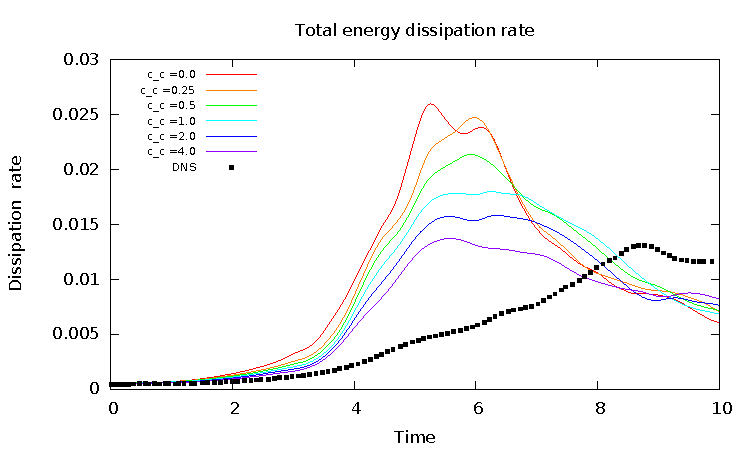
\includegraphics[width=0.75\textwidth]{Figures/TGV_OSS_ISS_tauc_tot.pdf}
     \vspace*{-0.3cm}
     \caption{Total energy dissipation rate.}
   \end{figure}}
 \only<4-5>{
    \begin{figure}
      \centering	
      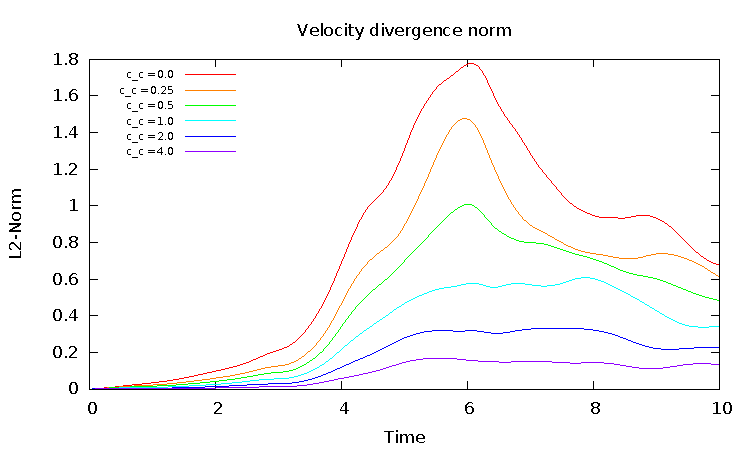
\includegraphics[width=0.75\textwidth]{Figures/TGV_OSS_ISS_tauc_div.pdf}
      \vspace*{-0.3cm}
      \caption{$\|\nabla\cdot\u\|$.}
    \end{figure}}  
 \only<6->{
   \begin{figure}
     \centering	
     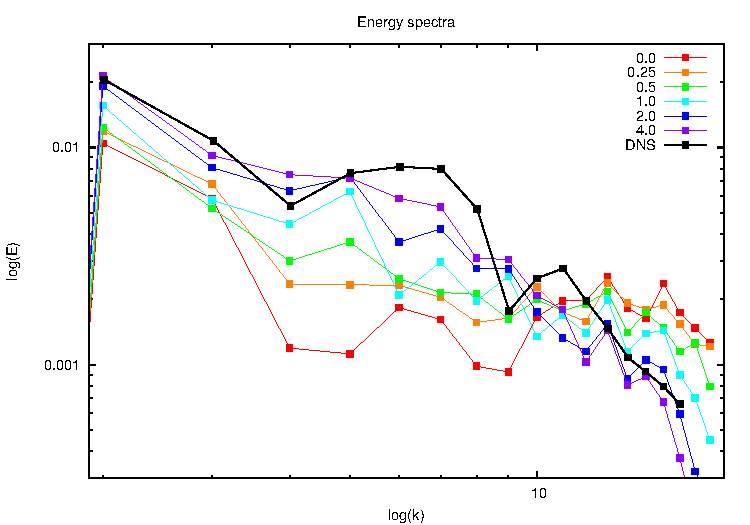
\includegraphics[width=0.65\textwidth]{Figures/TGV_OSS_ISS_tauc_spe.pdf}
     \vspace*{-0.3cm}
     \caption{Energy spectra.}
   \end{figure}}
 \begin{overlayarea}{\textwidth}{1.5cm}
 \vspace*{-0.5cm}
 \only<2-3>{
 \begin{itemize}
   	\item \alert<2>{Bad results} when $ c_c\rightarrow0 $.
   	\only<3>{\item Best option \alert<3>{$ c_c=4.0 $}.}
 \end{itemize}}
 \only<5>{
 \begin{itemize}
   	 \item \alert<5>{Incompressibility constraint not satisfied}.
 \end{itemize}}
 \only<7->{
 \begin{itemize}
   	\item \alert<7>{Overdissipation} on the \alert<7>{large scales} when $ c_c\rightarrow0 $.
   	\only<8>{\item \alert<8>{Infradissipation} on the \alert<8>{small scales} when $ c_c\rightarrow0 $.}
 \end{itemize}}
 \end{overlayarea}
\end{frame}

%=========================================================================================
% 3.3.3.TCF
% ----------------------------------------------------------------------------
\subsubsection{TCF}
%---------------------------------------------------------------------------
\begin{frame}[t]
\frametitle{TCF {\small Turbulent Channel Flow at $ Re_\tau=395 $}}
\textbf{Mean stream-wise velocity (models):}
 \vspace*{-0.3cm}
  \begin{figure}
    \centering	
    \only<1-3>{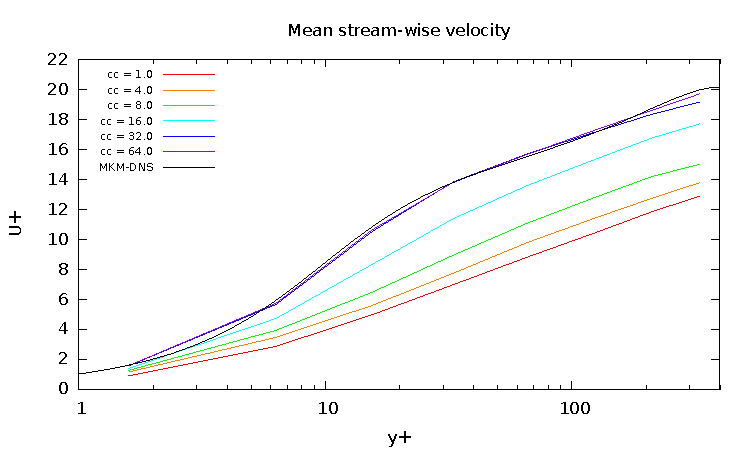
\includegraphics[width=0.75\textwidth]{Figures/tbt_TCF/umean}}
%    \only<4>{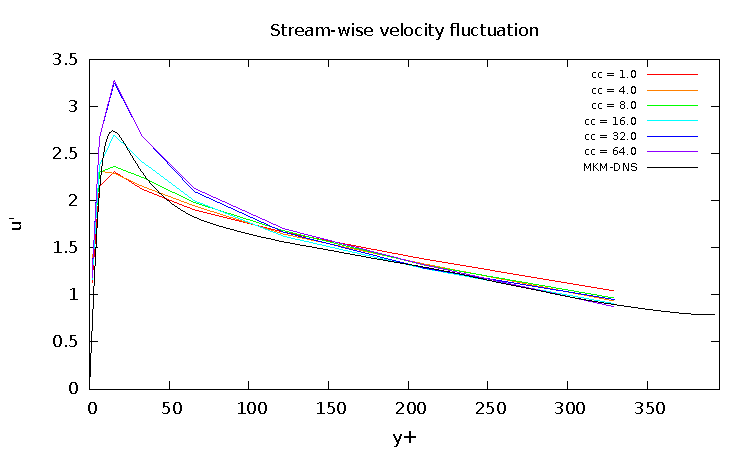
\includegraphics[width=0.75\textwidth]{Figures/tbt_TCF/ufluc}}
%    \only<5>{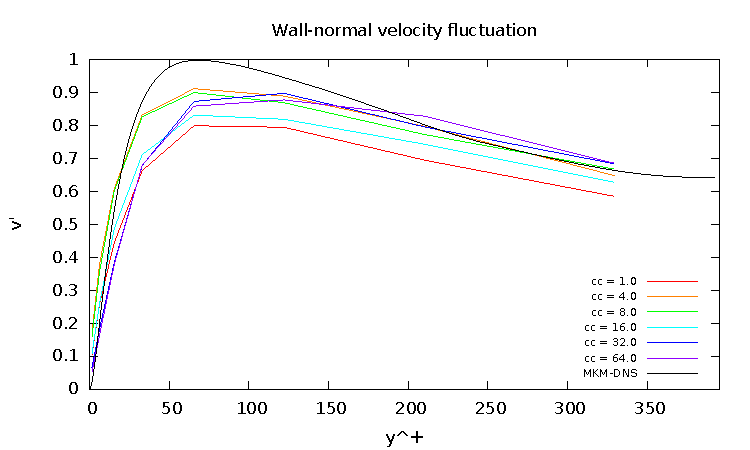
\includegraphics[width=0.75\textwidth]{Figures/tbt_TCF/vfluc}}
%    \only<6>{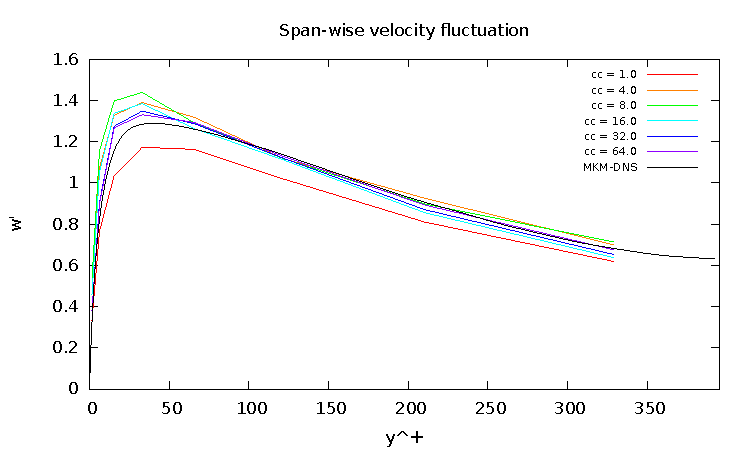
\includegraphics[width=0.75\textwidth]{Figures/tbt_TCF/wfluc}} 
  \end{figure}
  \vspace*{-0.5cm}
   \begin{overlayarea}{\textwidth}{1.5cm}
 \only<2->{
 \begin{itemize}
  	\item \alert<2>{Same behaviour} observed for TCF test
  	\only<3->{\item Best option \alert<3>{$ c_c=32.0 $}}
  \end{itemize}}
  \end{overlayarea}
\end{frame}

%=========================================================================================
% 3.4.CONCLUSIONS
% ----------------------------------------------------------------------------
\subsection{Conclusions}
%---------------------------------------------------------------------------
\begin{frame}
\frametitle{Mixed FE VMS Conclusions}
\vfill
\begin{itemize}
\item<1-> Scalable recursive block-preconditioners.
\item<2-> Sligthly better results for equal-order interpolations.
\item<3-> Mixed FE OSS the most efficient method. 
\item<4-> Mixed FE OSS keeps the index-2 DAE nature in time of the problem.
\end{itemize}
\vfill
\end{frame}
%---------------------------------------------------------------------------
\begin{frame}
\frametitle{Mixed FE VMS Limitations}
\vfill
\begin{itemize}
\item<1-> Strong dependency on the grad-div stabilization term.
\end{itemize}
\vfill
\end{frame}

%=========================================================================================
% 4.SRK
% ----------------------------------------------------------------------------
\section{Segregated Runge-Kutta}
\addtocounter{framenumber}{-1}
\frame{
\begin{minipage}[\textheight]{0.5\textwidth}
\vfill
\tableofcontents[currentsection,
				subsubsectionstyle=hide,
				sectionstyle=show/shaded, 
				subsectionstyle=show/show/hide]
\vfill
\end{minipage}
\begin{minipage}[\textheight]{0.4\textwidth}
  	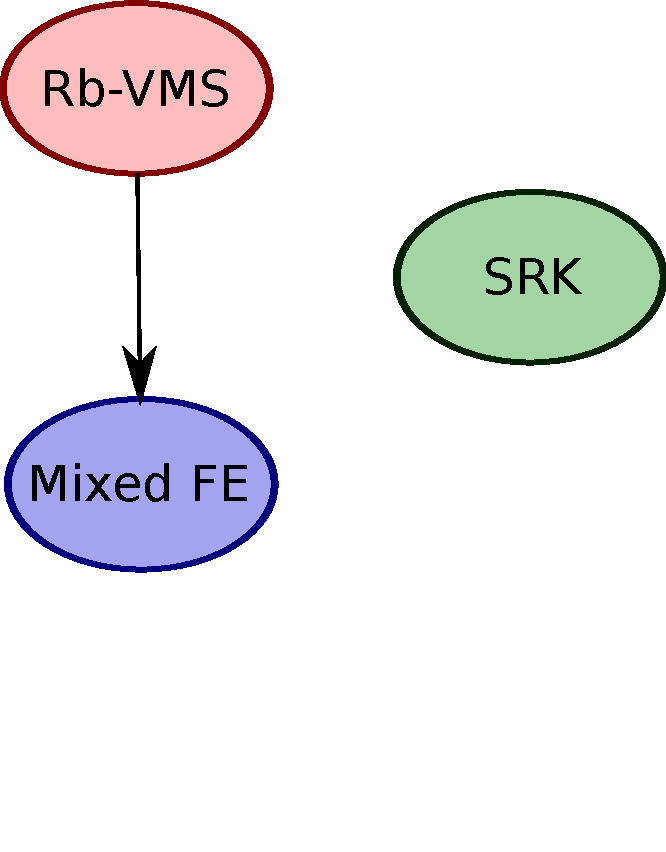
\includegraphics[width=1.1\textwidth]{Figures/index_3}
\end{minipage}
}
\begin{frame}
\frametitle{Motivation}
\vfill
\textbf{Step by step...}
\begin{itemize}
\item \algreen{1}{Residual-based VMS as LES models}
\item \algreen{1}{Mixed FE formulations LES}
\item \algreen{1}{High-order FE methods}
\alert<1>{\item High-order time integration schemes}
\alert<1>{\item Adaptive time stepping techniques}
\alert<1>{\item Velocity-pressure segregation}
\item Scalable solvers
\item Application
\end{itemize}
\vfill
\end{frame}

%=========================================================================================
% 4.1.FORMULATION
% ----------------------------------------------------------------------------
\subsection{Formulation}
%----------------------------------------------------------------------------------------
\begin{frame}[t]
\frametitle{Incomp. Navier Stokes equations}
\only<1-4>{Find $ \mathbf{u}$ and $p$ defined in $\Omega$}
\only<5->{Find $ \U$ and $\P$}
\only<1-4>{
\begin{align*}
\partial _{t}\mathbf{u}+ \mathbf{u}\cdot \mathbf{\nabla u}+\mathbf{
\nabla }p-\nu \nabla ^{2}\mathbf{u}& =\mathbf{f} \\
\mathbf{\nabla }\cdot \mathbf{u}& =0
\end{align*}}
\only<5>{
\begin{align*}
\dot{\U}+M^{-1}(K+C(\U))\U+ M^{-1}G\P&=\F,\\
D\U&= \G,
\end{align*}}
\only<6>{
\begin{align*}
&\dot{\U}+M^{-1}(K+C(\U))\U+ M^{-1}G\P=\F,\\
&-DM^{-1}G\P=DM^{-1}(K+C(\U)\U- \F) + \dot{\G},
\end{align*}}
with appropriate boundary conditions on $ \Gamma$.\vskip 0.3cm
\only<2->{
\begin{itemize}
\item<2-> \alert<2>{Laminar} case (no convection stabilization required).
\item<3-> Saddle-point structure (stability via \alert<3>{mixed FE}).
\item<4-> \alert<4>{Index-2 DAE} system (time integration with care)
\end{itemize}}
\end{frame}
%----------------------------------------------------------------------------------------
\begin{frame}
\frametitle{Velocity-pressure splitting}
\textbf{Existing methods: Fractional step / pressure segregation methods}
\begin{align*}
&\dot{\U}+M^{-1}(K+C(\U))\U+ M^{-1}G\alert{\P^*}=\F,&\mbox{in $(t^n,t^{n+1}]$,}\\
&-DM^{-1}G\P=DM^{-1}(K+C(\U)\U- \F) + \dot{\G},&\mbox{in $t^{n+1}$,}
\end{align*}
\only<1>{Some properties:
\begin{itemize}
\item $P^*$ extrapolation from previous time steps
\item Time-marching scheme for the momentum eq'on (ODE system!)
\item Velocity and pressure computations are segregated
\item A must for computational efficiency (coercive blocks)
\item 2nd order splitting error ( $>2$ unstable)
%\item Better preconditioning strategies (Poisson-type solvers)
\end{itemize}}
\onslide<2->{\emph{High-order} time integration:
\begin{itemize}
\item Fractional step techniques + (e.g.) Runge-Kutta for momentum equation: [Nikitin'06; Knikker'09; Kampanis et al'06...]
\item Introduce segregation error (2nd order)
\end{itemize}}
\onslide<3>{Drawbacks: 
\begin{itemize}
\item Segregation error can jeopardize high order time integrators
\item Effect of segregation on pressure error unclear (not reported in literature)
\end{itemize}}
\end{frame}
%----------------------------------------------------------------------------------------
\begin{frame}
\frametitle{Velocity-pressure splitting}
\textbf{Existing methods: Half-explicit RK methods (HERK)}
\vspace{-0.5cm}
\begin{overprint}
\onslide<1>
\begin{align*}
%\label{eq:IMEX_NS_iup_HE}
\frac{1}{\delta t}\U_i=\frac{1}{\delta t}\U_n + \sum_{j=1}^{i-1}\hat{a}_{ij} M^{-1} (K U_j + C(U_j) U_j + G P_j), \\
 D \U_i = \G(t_i),
\end{align*}
\onslide<2->
\begin{align*}
%\label{eq:IMEX_NS_fup_HE}
\frac{1}{\delta t}\U_i=\frac{1}{\delta t}\U_n - \sum_{j=1}^{i-1}\hat{a}_{ij} M^{-1} (K U_j + C(U_j) U_j + G P_j), \\
D \U_n - \delta t \sum_{j=1}^{i-1}\hat{a}_{ij} DM^{-1}(K U_j + C(U_j) U_j + G P_j) = \G(t_i).
\end{align*}
\end{overprint}
\vspace{0.3cm}
\only<2>{\emph{High-order} time integration:
\begin{itemize}
\item Recently applied to the Navier-Stokes equations [Sanderse \& Koren'12]
\item Velocity-pressure segregation by the time integrator 
\item No additional splitting needed (high-order feasible, not spoiled)
\end{itemize}}
\only<3>{Drawbacks: 
\begin{itemize}
\item All terms must be treated explicitly (viscous + convective terms)
\item Implicit treatment of interest when $\delta t_{\rm CFL}$ smaller than finest time scales of interest [Verstappen \& Veldman'03; Vreman \& Kuerten'14]
\item A straightforward application with implicit/IMEX integrators leads to, e..g, $D (M + \delta t K_V)^{-1} G$ matrix for the pressure (not affordable)
\end{itemize}}
\end{frame}
%----------------------------------------------------------------------------------------
\begin{frame}
\frametitle{Segregated RK methods}
\vfill
\begin{itemize}
\item<1-> \textbf{Observation:} No implicit / IMEX high-order integrators with implicit velocity-pressure segregation
\item<2-> \textbf{Target:} Develop such algorithms (of RK type)
\item<3-> \textbf{Result:} Segregated RK methods [Colom\'es \& SB'15]
\end{itemize}
\vfill
\end{frame}
%----------------------------------------------------------------------------------------
\begin{frame}
\frametitle{Segregated RK methods}
\textbf{The idea:}
\begin{enumerate}
\item Consider the projected momentum eq'on on the discretely divergence free space
\item<4-> Integrate the resulting ODE system w/ preferred IMEX RK method (diagonally implicit)...
\item<5-> $\mathcal{G}$ must include $G(DM^{-1}G)^{-1} \left( DM^{-1}(K+C(\U)\U - \F)+ \dot{\G} \right)$ for velocity-pressure segregation
\item<6-> The rest of terms can be treated implicitly / explicitly
\end{enumerate}
\begin{overprint}
\onslide<1>
\begin{align*}
&M\dot{\U}+(K+C(\U))\U+ G\P=\F,\\
&D\U= \G
\end{align*}
\onslide<2>
\begin{align*}
&M\dot{\U}+(K+C(\U))\U+ G\P=\F,\\
&-DM^{-1}G\P=DM^{-1}(K+C(\U)\U- \F) + \dot{\G}
\end{align*}
\onslide<3>
\begin{align*}
\label{eq:NS_galerkin_ou}
&M\dot{\U}+ P(K+C(\U))\U  = P\F + G(DM^{-1}G)^{-1} \dot{\G}, \\ & \qquad \hbox{with } \ P := 
(I - G(DM^{-1}G)^{-1}DM^{-1}) \end{align*}
\onslide<4->
\begin{align*}
&
M\dot{\U}=\mathcal{F}(\U)+\mathcal{G}(\U), \qquad \mathcal{F}: \hbox{ implicit terms},  \quad \mathcal{G}: \hbox{ explicit ones} %,\\
%&\dot{\G} + DM^{-1}(K+C(\U))\U+DM^{-1}G\P=DM^{-1}\F.
\end{align*}
\end{overprint}
\end{frame}
%----------------------------------------------------------------------------------------
\begin{frame}
\frametitle{Segregated RK methods}
It leads to the time-discrete algorithm:
\begin{align*}
\frac{1}{\delta t}M\U_i=\frac{1}{\delta t}M\U_n+\sum_{j=1}^ia_{ij}\mathcal{F}(\U_j)+\sum_{j=1}^{i-1}\hat{a}_{ij}\mathcal{G}(\U_j)
\end{align*}
After re-ordering (pressure again):
\begin{align*}
%\label{eq:IMEX_NS_p}
\frac{1}{\delta t}M\U_i=\frac{1}{\delta t}M\U_n+\sum_{j=1}^ia_{ij}\mathcal{F}(\U_j)+\sum_{j=1}^{i-1}\hat{a}_{ij}  \tilde{\mathcal{G}}(\U_j,\P_j),\\
- DM^{-1}G (\P_i)=DM^{-1}((K+C(\U_i))\U_i - \F(t_i)) +\dot{\G}(t_i)
\end{align*}
\begin{overprint}
\onslide<2>
\begin{itemize}
\item Viscous / convective can be treated implicitly / explicitly
\begin{align*}
&\mathcal{F}(\U) :=-K\U + \F - C(\U)\U, \qquad &&\tilde{\mathcal{G}(\U,P)} = -G P \qquad 
\hbox{ or } \\
&\mathcal{F}(\U) :=-K\U + \F,  \qquad && \tilde{\mathcal{G}}(\U,P) = - C(\U)\U - G P
\end{align*}
\end{itemize}
\onslide<3>
Features:
\begin{enumerate}
\item Segregation at the time integration level (no additional splitting)
\item High order achievable (the one of the ODE RK integration)
\item Implicit LES turbulent model (stabilization terms)
\end{enumerate}
\end{overprint}
\end{frame}
%----------------------------------------------------------------------------------------
\begin{frame}
\frametitle{Some properties}
\vfill
Some proved results [Colom\'es \& SB'15]:
\begin{itemize}
\item HERK and SRK methods are \emph{equivalent} for full explicit treatment
\item However, in SRK methods we are not enforcing implicitly the constraint...
\item We have proved that $D U(t) = G$ as soon as strongly imposed velocity traces are polynomials or order $p$ and $D U(0) = G(0)$
\\ {\small ($p$: order of IMEX RK time integrator) }
\item Equivalent when weakly enforced boundary conditions (dG)
\item Equal-order \& optimal velocity-pressure methods (of interest in FSI, etc.)
\end{itemize}
\vfill
\end{frame}



%=========================================================================================
% 4.2.NUMERICAL EXPERIMENTS
% ----------------------------------------------------------------------------
\subsection{Numerical experiments}
\begin{frame}[t]
\frametitle{Numerical experiments}
\vfill
Manufactured analytical solutions:
\begin{itemize}
\item Simple $ sin(t)\cdot\exp(t) $ function.
\end{itemize}
\vspace{1cm}
Laminar benchmark:
\begin{itemize}
\item 2D Laminar flow around a cylinder.
\end{itemize}
\vfill
\end{frame}

%=========================================================================================
% 4.2.1.ANALYTICAL
% ----------------------------------------------------------------------------
\subsubsection{Analytical solution}
%----------------------------------------------------------------------------------------
\begin{frame}
  \frametitle{Manufactured analytical solution}
  \textbf{Problem setting:}
  \begin{itemize}
    \itemsep-0.10cm
 	\item Analytical solution: \begin{align*}
 	&\u(x,y,t) = \left[\begin{array}{c}
 	 	x\\
 	 	-y
 	 	\end{array}\right]\sin(\frac{\pi}{10}t)\exp(\frac{t}{25}),\\
 	&p(x,y) = x+y.
 	\end{align*}
  	\item $Re=1/10/100$. 
  	\item Different IMEX Butcher tableaus with 1st, 2nd and 3rd order.
  \end{itemize}
\end{frame}
%----------------------------------------------------------------------------------------
\begin{frame}
\frametitle{Manufactured analytical solution}
\only<1>{
\textbf{Implicit convection:}
\begin{figure}[h!]
\centering
\subfigure[Velocity convergence, $\nu=0.01$]{\label{fig:IMEX_implcnv_RK_vel_analytical_nu0.01}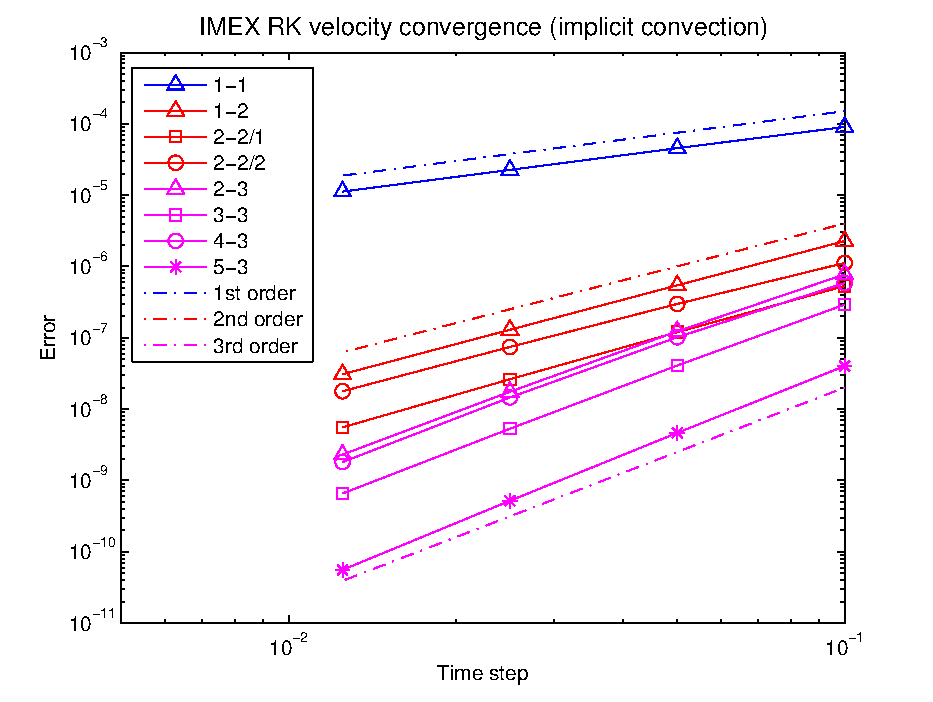
\includegraphics[width=0.49\textwidth]{Figures/vel_nu1dot0E-02_implconv}}    
\subfigure[Pressure convergence, $\nu=0.01$]{\label{fig:IMEX_implcnv_RK_pre_analytical_nu0.01}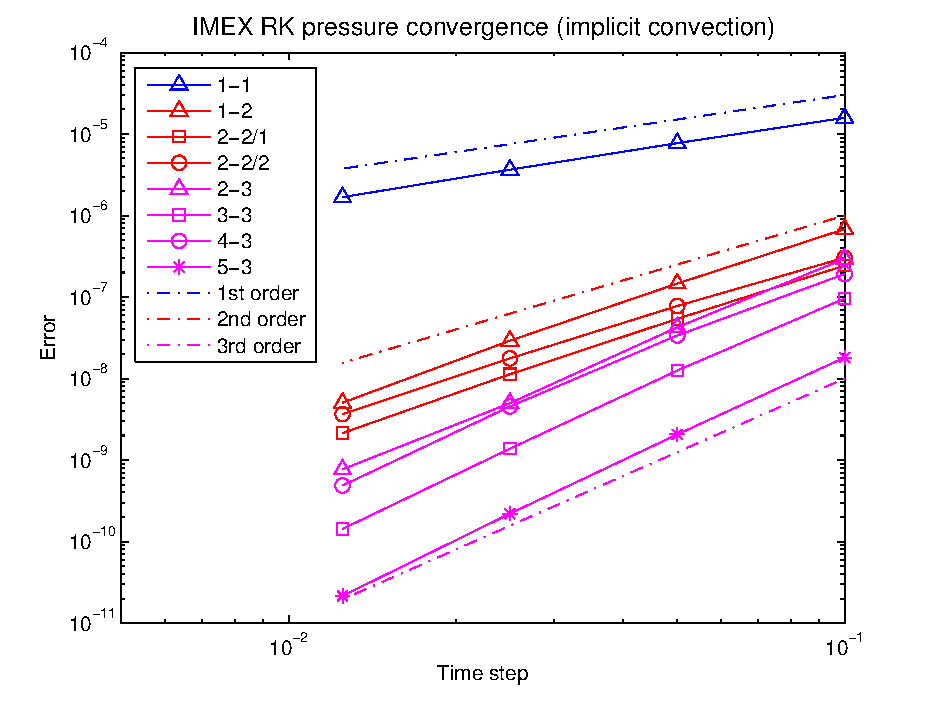
\includegraphics[width=0.49\textwidth]{Figures/pre_nu1dot0E-02_implconv}}
\caption{Fully implicit SRK.}
\label{fig:IMEX_implcnv_RK_analytical}
\end{figure}}
\only<2>{
\textbf{Explicit convection:}
\begin{figure}[h!]
\centering
\subfigure[Velocity convergence, $\nu=0.01$]{\label{fig:IMEX_explcnv_RK_vel_analytical_nu0.01}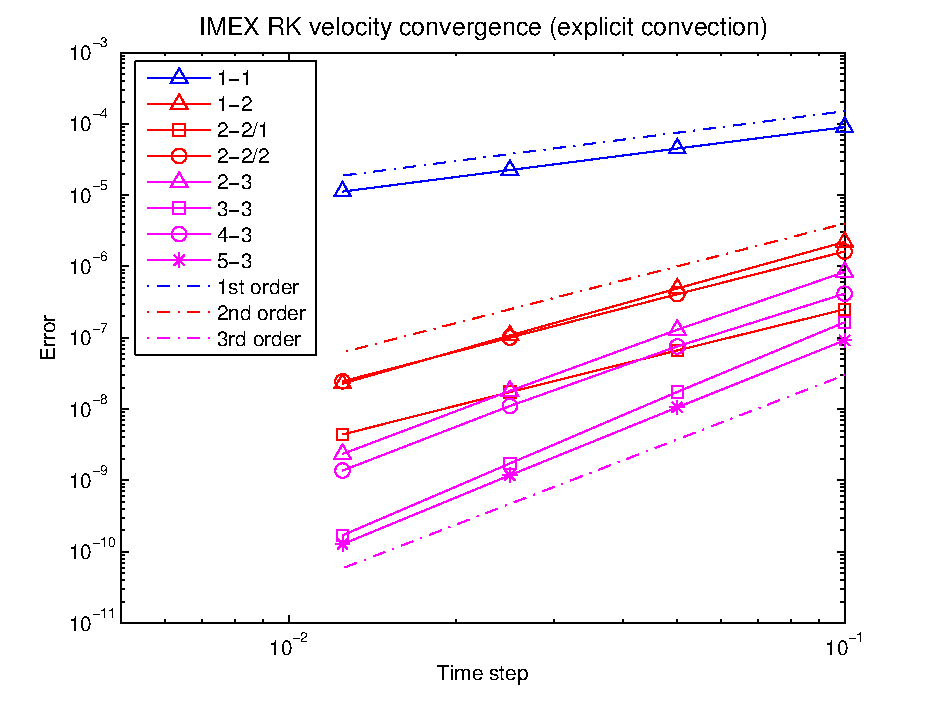
\includegraphics[width=0.49\textwidth]{Figures/vel_nu1dot0E-02_explconv}}    
\subfigure[Pressure convergence, $\nu=0.01$]{\label{fig:IMEX_explcnv_RK_pre_analytical_nu0.01}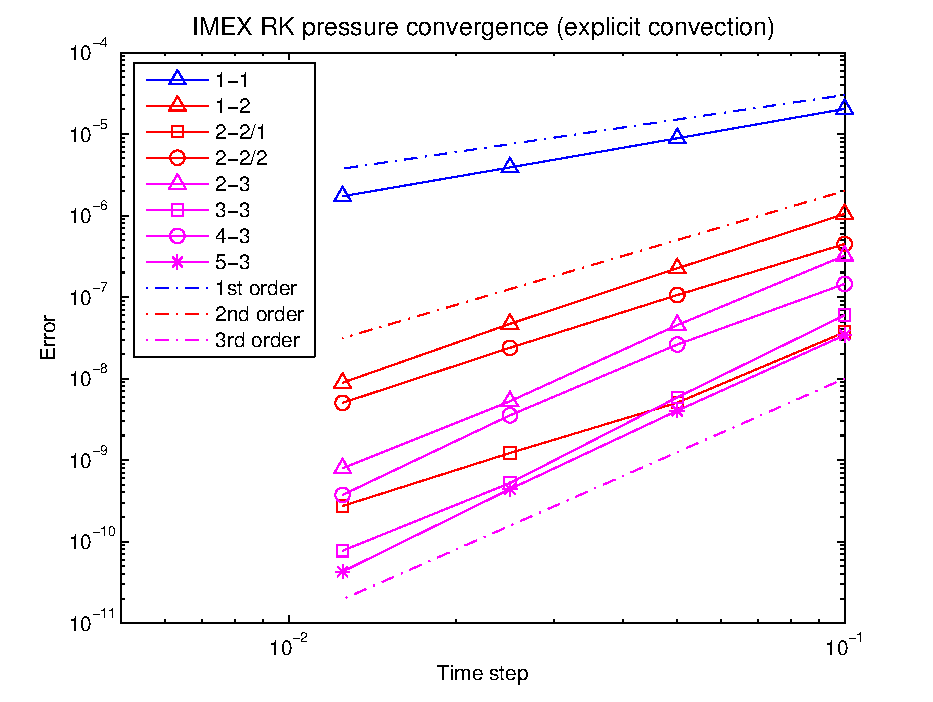
\includegraphics[width=0.49\textwidth]{Figures/pre_nu1dot0E-02_explconv}}
\caption{SRK convergence with convection integrated explicitly and diffusion integrated implicitly.}
\label{fig:IMEX_explcnv_RK_analytical}
\end{figure}}
\end{frame}




%=========================================================================================
% 4.2.2.CYLINDER
% ----------------------------------------------------------------------------
\subsubsection{Flow around a cylinder}
%----------------------------------------------------------------------------------------
\begin{frame}
  \frametitle{2D Laminar flow around a cylinder}
  \textbf{Problem setting:}
  \begin{itemize}
 	\item Widely used benchmark.
  	\item $Re=100$. 
  	\item Time convergence.
  	\item Drag and Lift coefficients.
  \end{itemize}
  \begin{figure}
   \centering	  
   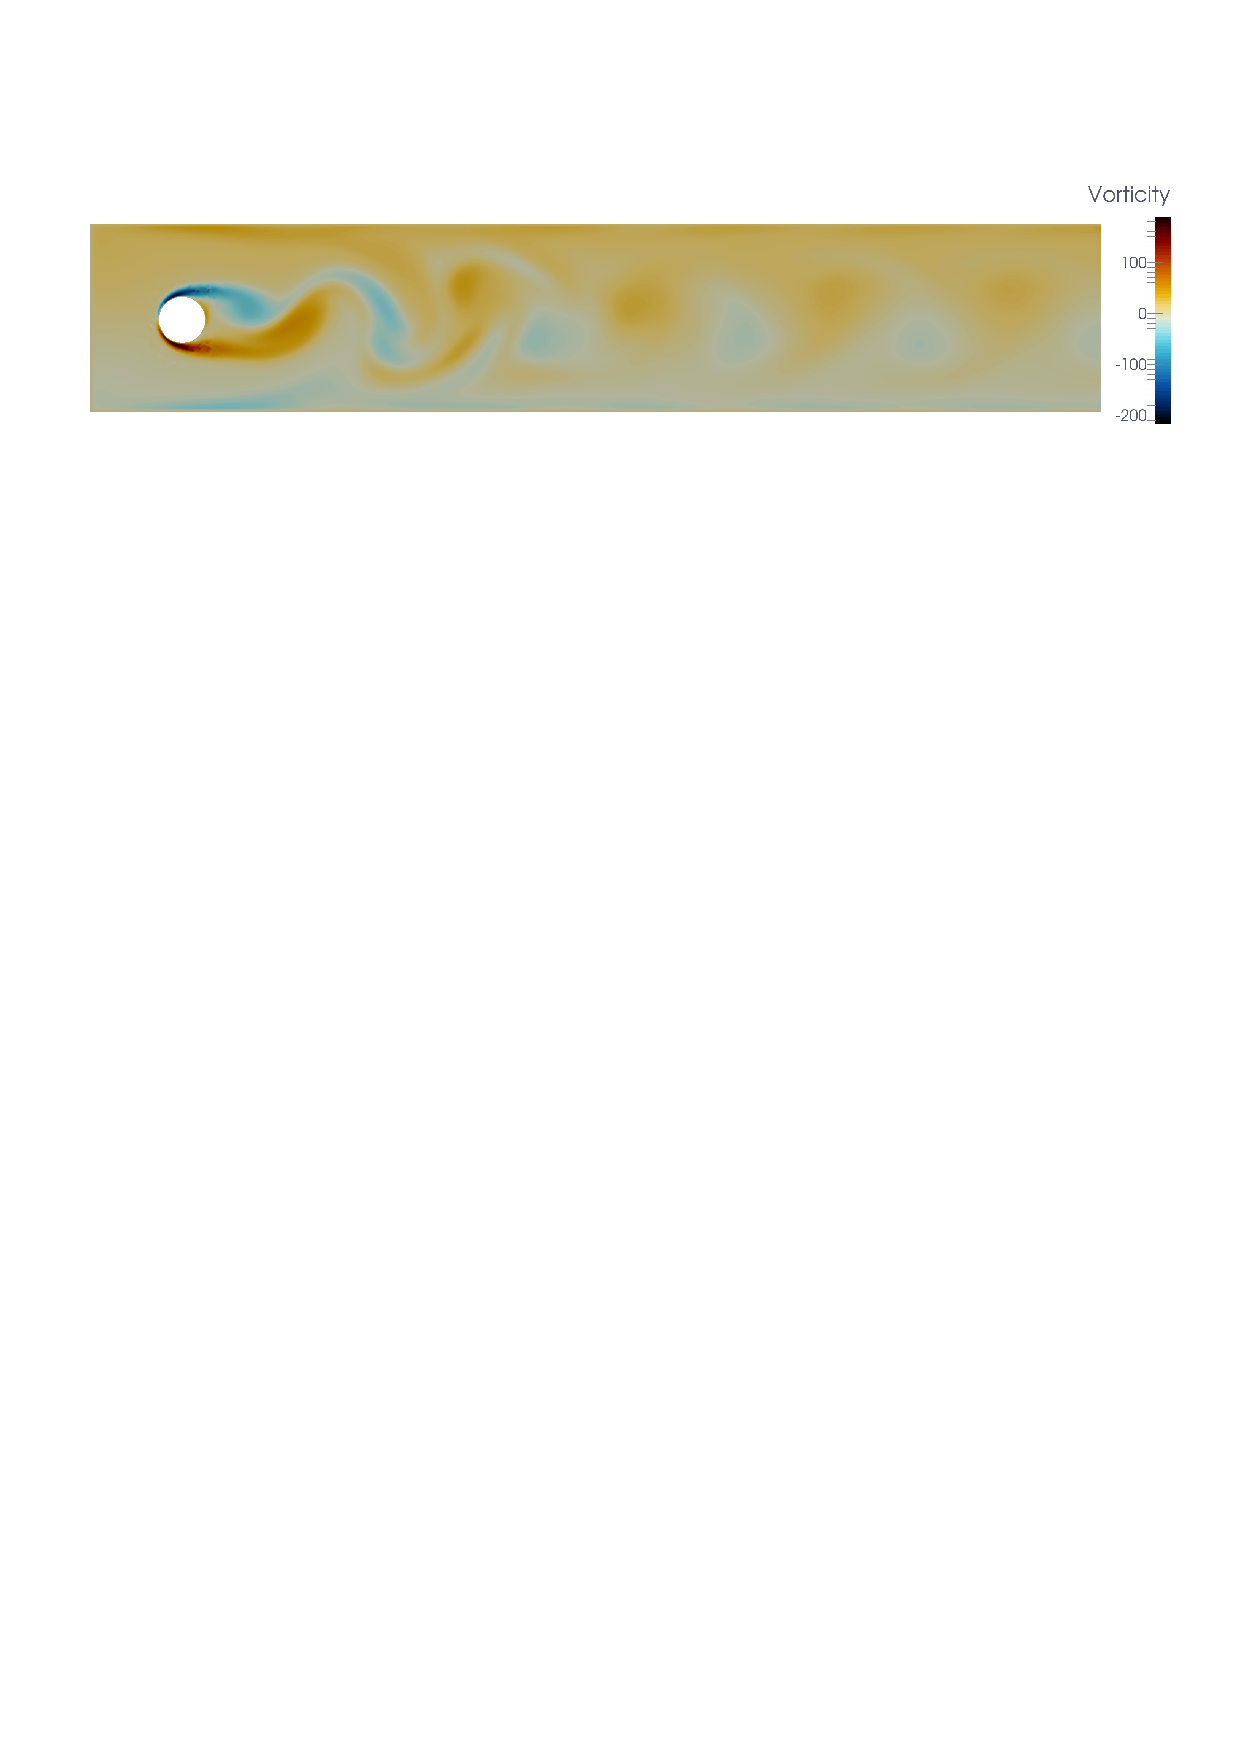
\includegraphics[clip=true,trim=1.5cm 22.5cm 1cm 3cm,width=1.0\textwidth]{Figures/vorticity}
     \caption{Vorticity field at $t=8.0$.}
     \label{fig:Cyl_vorti}
  \end{figure}
\end{frame}
%----------------------------------------------------------------------------------------
\begin{frame}
\frametitle{2D Laminar flow around a cylinder}
\textbf{Implicit \& explicit convection:}
\begin{figure}[h!]
  \centering
  \subfigure[Velocity convergence]{\label{fig:IMEX_RK_vel_cyl_impl_expl}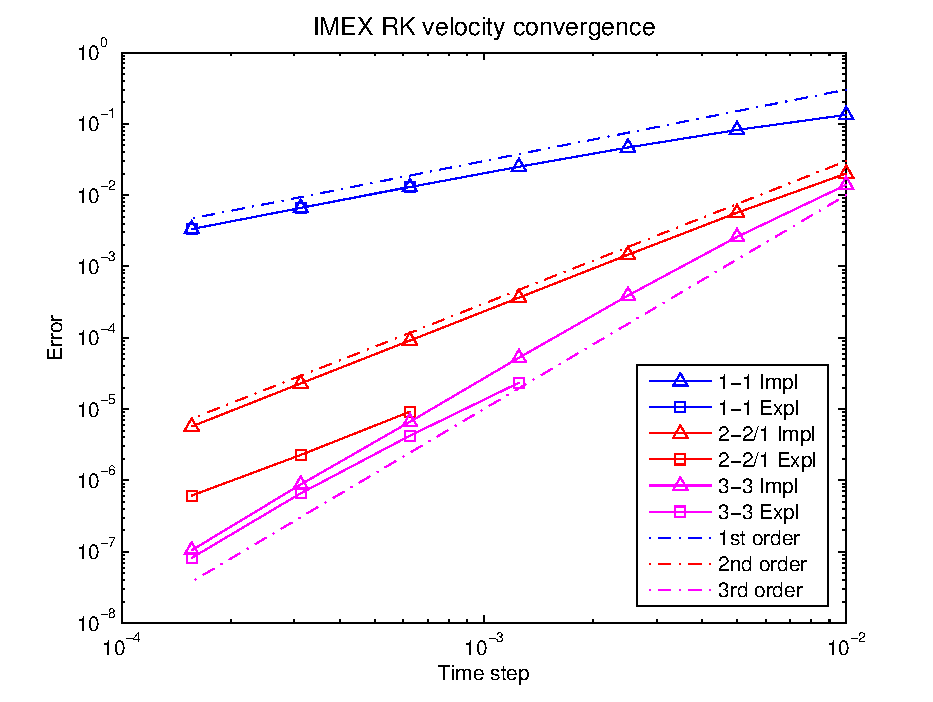
\includegraphics[width=0.49\textwidth]{Figures/vel_impl_expl}}    
  \subfigure[Pressure convergence]{\label{fig:IMEX_RK_pre_cyl_impl_expl}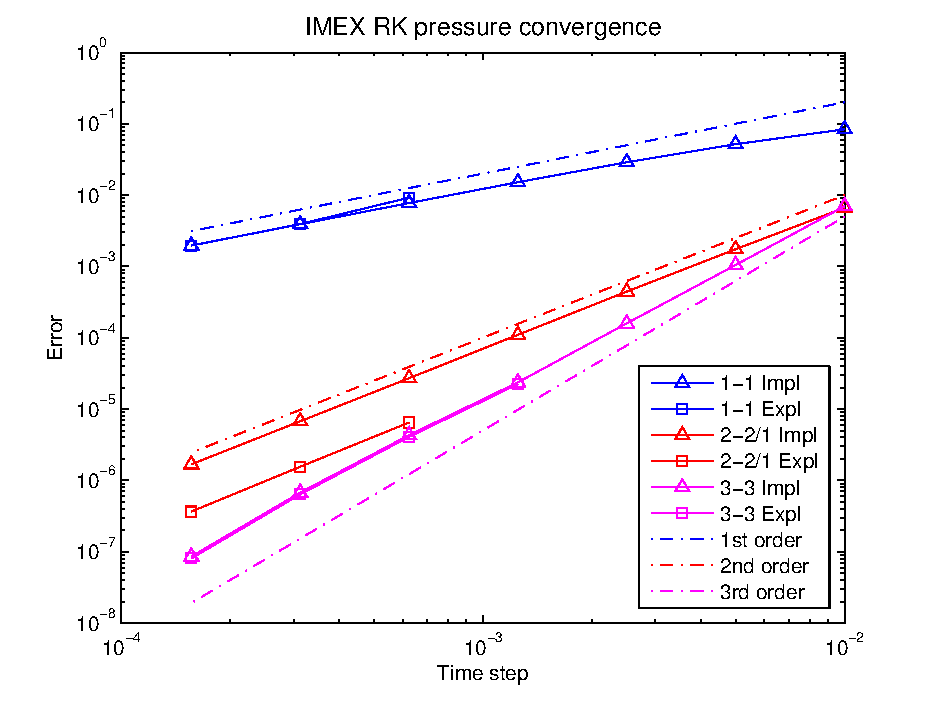
\includegraphics[width=0.49\textwidth]{Figures/pre_impl_expl}}
  \caption{Fully implicit and IMEX-SRK convergence rate comparison.}
  \label{fig:IMEX_RK_cyl_conv_impl_expl}
\end{figure}
\end{frame}




%=========================================================================================
% 4.3.CONCLUSIONS
% ----------------------------------------------------------------------------
\subsection{Conclusions}
%---------------------------------------------------------------------------
\begin{frame}
\frametitle{Segregated Runge-Kutta Conclusions}
\vfill
\begin{itemize}
\item<1-> Velocity-pressure segregated by the time integrator (IMEX RK)
\item<2-> No additional splitting needed
\item<3-> Equal order in time (pressure error not spoiled)
\end{itemize}
\vfill
\end{frame}
%---------------------------------------------------------------------------
\begin{frame}
\frametitle{Segregated Runge-Kutta Limitations}
\vfill
\begin{itemize}
\item<1-> Only for index-2 DAE. 
\item<2-> Not applicable for equal-order stabilization methods.
\end{itemize}
\vfill
\end{frame}

%=========================================================================================
% 5.SVMS
% ----------------------------------------------------------------------------
\section{Segregated VMS}
\addtocounter{framenumber}{-1}
\frame{
\begin{minipage}[\textheight]{0.5\textwidth}
\vfill
\tableofcontents[currentsection,
			  	subsubsectionstyle=hide,
				sectionstyle=show/shaded, 
				subsectionstyle=show/show/hide]
\vfill
\end{minipage}
\begin{minipage}[\textheight]{0.4\textwidth}
  	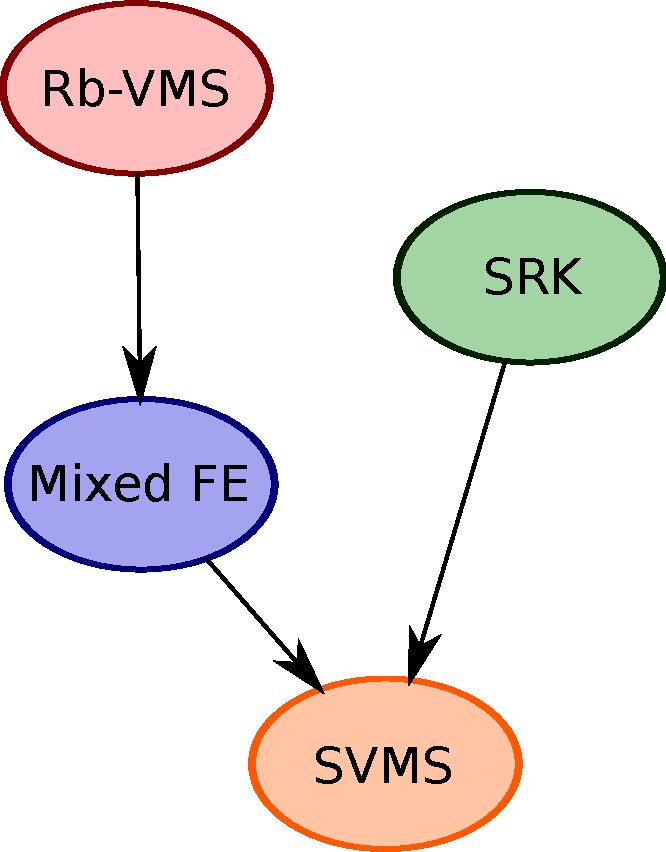
\includegraphics[width=1.1\textwidth]{Figures/index}
\end{minipage}
}
\begin{frame}
\frametitle{Motivation}
\vfill
\textbf{Step by step...}
\begin{itemize}
\item \algreen{1}{Residual-based VMS as LES models}
\item \algreen{1}{Mixed FE formulations LES}
\item \algreen{1}{High-order FE methods}
\algreen{1}{\item High-order time integration schemes}
\algreen{1}{\item Adaptive time stepping techniques}
\algreen{1}{\item Velocity-pressure segregation}
\alert<1>{\item Scalable solvers}
\alert<1>{\item Application}
\end{itemize}
\vfill
\end{frame}
%-----------------------------------------------------------------------------------------
\begin{frame}
\frametitle{Looking backward...}
\vfill
\begin{overlayarea}{\textwidth}{0.5\textheight}
\only<1-3>{
\textbf{VMS as LES models:}} \only<1>{\alert<1>{Residual-based VMS} methods}\only<2-3>{\alert<2-3>{Mixed FE VMS} methods}
\only<1>{
\begin{itemize}
\item Velocity + pressure stabilization, applied to equal-order FEs
\item Intensively tested methods (several works in the literature)
\item Nature of the problem changes, not DAE-2 type (!)
\item It prevents us to use segregated RK methods
\end{itemize}}
\only<2-3>{\begin{itemize}
\item Only the term that we need, i.e., convection stabilization
\item To keep accuracy, we use orthogonal projections ($ \mathcal{P}_h^\perp $)
\item Many choices for the $\mathcal{P}_h$ projector: local, global (OSS)
\item Discrete problem still index-2 DAE
\item Segregated RK schemes can be used
\end{itemize}
\only<3>{Now, we can use \alert<3>{Segregated RK methods for ILES of turbulent flows}}}
\end{overlayarea}
\vfill
\end{frame}

%=========================================================================================
% 5.1.FORMULATION
% ----------------------------------------------------------------------------
\subsection{Formulation}
%----------------------------------------------------------------------------------------
\begin{frame}[t]
\frametitle{Formulation}
\textbf{OSS-ISS}: \only<1-2>{Semi-discrete form}
\begin{enumerate}
\item<3-> Consider the projected momentum eq'on on the discretely divergence free space
\item<4-> Integrate the resulting ODE system w/ preferred IMEX RK method (diagonally implicit)...
\item<5-> $\mathcal{G}$ must include $G(DM^{-1}G)^{-1} \left( DM^{-1}(K+C(\U)+A_\tau)\U+B_\tau\ETA - \F_u) \right)$ for velocity-pressure segregation
\item<6-> We treat the projection term implicit or explicit, according the convective term.
\end{enumerate}
\begin{overprint}
\only<1>{
\begin{equation*}
\left[\begin{array}{c}
M\overset{.}{\U}\\
\mathbf{0}\\
\mathbf{0}
\end{array}\right]+\left[\begin{array}{ccc}
K+C(\U)+A_\tau&G&B_\tau\\
D&\alert<4>{0}&0\\
-B_\tau^T&0&M_\tau
\end{array}\right]\left[\begin{array}{c}
\U\\
\P\\
\ETA
\end{array}\right]=\left[\begin{array}{c}
\F_u\\
\mathbf{0}\\
\mathbf{0}
\end{array}\right],
\end{equation*}}
\only<2>{
\begin{align*}
M\dot{\U}+(K+C(\U)+A_\tau)\U+G\P+B_\tau\ETA&=\F_u,\\
M_\tau\ETA-B_\tau^T\U&=\mathbf{0},\\
D\U&=\mathbf{0}.
\end{align*}}
\only<3>{
\begin{align*}
&M\dot{\U}+(K+C(\U)+A_\tau)\U+G\P+B_\tau\ETA=\F_u,\\
&M_\tau\ETA-B_\tau^T\U=\mathbf{0},\\
&-DM^{-1}G\P=DM^{-1}(K+C(\U)\U+B_\tau\ETA- \F_u).
\end{align*}}
\only<4->{
\begin{align*}
&
M\dot{\U}=\mathcal{F}(\U\only<4-6>{,\alert<6>{\ETA}})+\mathcal{G}(\U\only<7>{,\alert<7>{\ETA}},\alert<5>{\P}), \qquad \mathcal{F}: \hbox{ implicit terms},  \quad \mathcal{G}: \hbox{ explicit ones} \\
&M_\tau\ETA-B_\tau^T\U=\mathbf{0},\\
&-DM^{-1}G\P=DM^{-1}((K+C(\U)+A_\tau)\U+B_\tau\ETA- \F_u).
\end{align*}}
\end{overprint}
\end{frame}
%----------------------------------------------------------------------------------------
\begin{frame}[t]
\frametitle{Final discrete problem}
At each stage of the Runge-Kutta scheme: (explicit convective term and projection version)
\begin{align*}
\only<1>{&\frac{1}{\delta t}M\U_i=\frac{1}{\delta t}M\U_n+\sum_{j=1}^ia_{ij}\mathcal{F}(\U_j)+\sum_{j=1}^{i-1}\hat{a}_{ij}  \mathcal{G}(\U_j,\ETA_j,\P_j),}
\only<2->{&\alert<3>{\left(\frac{1}{\delta t}M+a_{ii}K\right)}\U_i=\frac{1}{\delta t}M\U_n+\sum_{j=1}^{i-1}\left[a_{ij}\mathcal{F}(\U_j)+\hat{a}_{ij}  \mathcal{G}(\U_j,\ETA_j,\P_j)\right],}\\
&\alert<4>{M_\tau}\ETA_i-B_\tau^T\U_i=\mathbf{0},\\
&- \alert<5>{DM^{-1}G}(\P_i)=DM^{-1}((K+C(\U_i)+A_\tau)\U_i+B_\tau\ETA_i - \F_u(t_i)).
\end{align*}
\only<3->{
\begin{itemize}
\item<3-> \alert<3>{Elasticity-type} matrix for the momentum equation.
\item<4-> \alert<4>{Mass-type} matrix for the projection equation.
\item<5-> \alert<5>{Darcy-type} system for the pressure equation.
\end{itemize}}
\end{frame}

%=========================================================================================
% 5.2.LARGE SCALE
% ----------------------------------------------------------------------------
\subsection{Large-scale solvers}
%----------------------------------------------------------------------------------------
\begin{frame}
\frametitle{Large scale simulations} 
\begin{overprint}
\onslide<1->{
\textbf{Momentum system matrix:} $\frac{1}{\delta t}M+a_{ii}K$
\begin{itemize}
\item Multilevel/overlapped Balancing domain decomposition (BDDC) for $M + \delta t K$
\item Excellent weak scalability results (up to $ \sim 460,000 $ IBM BG/Q cores) [Badia \textit{et al} '15]
\end{itemize} }
\onslide<2->{
\textbf{Pressure system matrix:} $D M^{-1} G$
\begin{itemize}
\item Spectrally equivalent to standard Laplacian $L_p$
\item Written as 
\begin{align*}
\left[ 
\begin{array}{cc}
M & G \\ 
D & 0
\end{array}
\right] \qquad \hbox{preconditioned w/} \qquad
\left[ 
\begin{array}{cc}
M & 0 \\ 
0 & L_p
\end{array}
\right] 
\end{align*}
\item Multilevel/overlapped Balancing domain decomposition (BDDC) for $L_p$
\item Excellent weak scalability results (up to $ \sim 460,000 $ IBM BG/Q cores) [Badia \textit{et al} '15]
\end{itemize}}
\end{overprint}
\end{frame}

%=========================================================================================
% 5.3.NUMERICAL EXPERIMENTS
% ----------------------------------------------------------------------------
\subsection{Numerical experiments}
\begin{frame}[t]
\frametitle{Numerical experiments}
\vfill
Three different turbulent benchmarks:
\begin{itemize}
\item Taylor-Green Vortex (TGV) flow
\item Turbulent Channel Flow (TCF)
\item Flow around a NACA profile
\end{itemize}
\vfill
\end{frame}

%=========================================================================================
% 5.3.1.TGV
% ----------------------------------------------------------------------------
\subsubsection{TGV}
%----------------------------------------------------------------------------------------
\begin{frame}
 \frametitle{TGV {\small Taylor-Green Vortex flow}}
 \textbf{Monolithc vs Segregated Runge-Kutta:}
 \vspace*{-0.3cm}
   \begin{figure}
     \centering	
     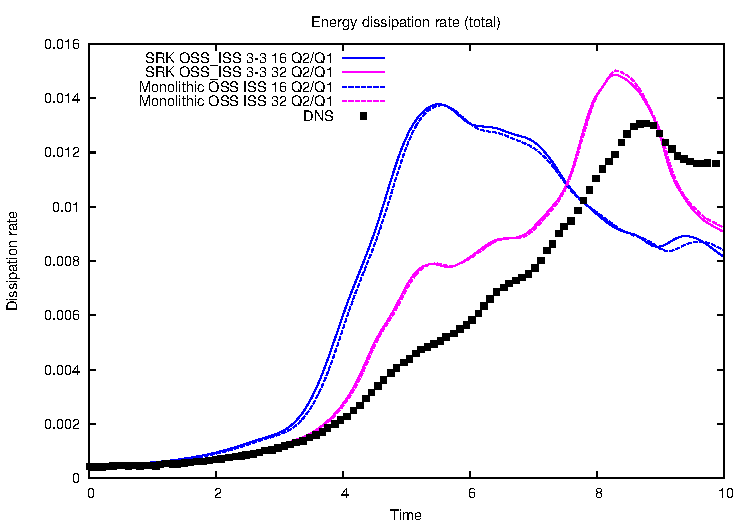
\includegraphics[width=0.65\textwidth]{Figures/plt_tg3d_tot.pdf}
     \vspace*{-0.3cm}
     \caption{Total energy dissipation rate}
   \end{figure}
 \begin{overlayarea}{\textwidth}{1.5cm}
 \only<2->{
 \vspace*{-0.5cm}
 \begin{itemize}
   	\item Almost \alert<2>{Identical results} obtained with Crank-Nicolson.
   	\only<3->{\item \alert<3>{IMEX and adaptive} time stepping.}
  \end{itemize}}
  \end{overlayarea}
\end{frame}
%----------------------------------------------------------------------------------------
\begin{frame}
 \frametitle{TGV {\small Taylor-Green Vortex flow}}
 \textbf{Weak scalability:}
 \vspace*{-0.1cm}
   \only<1-3>{
   \begin{figure}
     \centering	
     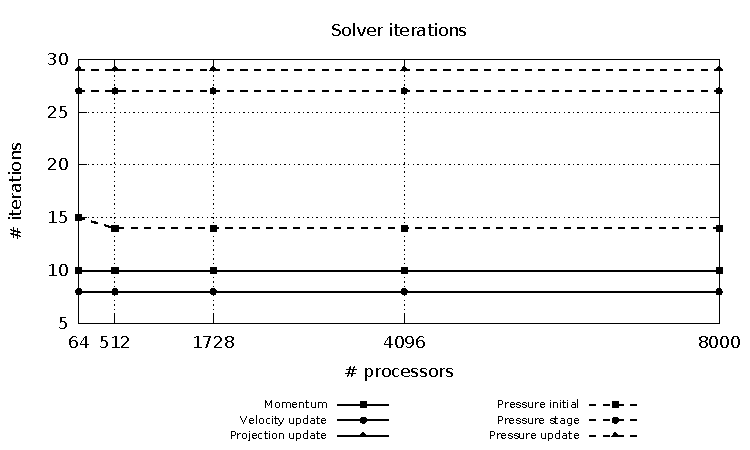
\includegraphics[width=0.75\textwidth]{Figures/iter_12_ce.pdf}
     \vspace*{-0.3cm}
     \caption{Solver iterations}
   \end{figure}}
   \only<4->{
   \begin{figure}
     \centering	
     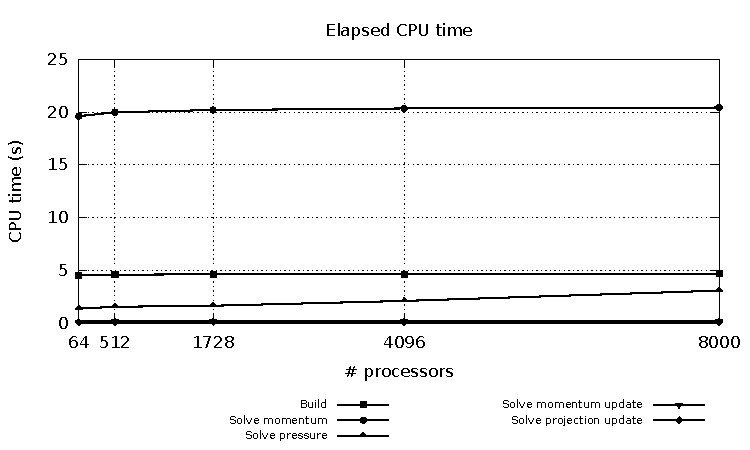
\includegraphics[width=0.75\textwidth]{Figures/time_12_ce.pdf}
     \vspace*{-0.3cm}
     \caption{CPU time}
   \end{figure}}
 \begin{overlayarea}{\textwidth}{1.5cm}
 \vspace*{-0.5cm}
 \only<2-3>{
 \begin{itemize}
   	\item \alert<2>{Perfect scalability} in terms of solver iterations.
   	\only<3->{\item \alert<3>{Darcy-type} problem requires \alert<3>{more iterations}.}
  \end{itemize}}
 \only<5->{
 \begin{itemize}
   	\item \alert<5>{Perfect scalability} in CPU time consumed.
   	\only<6->{\item \alert<6>{Momentum} problem requires \alert<6>{more time}.}
  \end{itemize}}
  \end{overlayarea}
\end{frame}

%=========================================================================================
% 5.3.2.TCF
% ----------------------------------------------------------------------------
\subsubsection{TCF}
%---------------------------------------------------------------------------
\begin{frame}[t]
\frametitle{TCF {\small Turbulent Channel Flow at $ Re_\tau=395 $}}
\textbf{LES for wall bounded flows?}
\vfill
\onslide<1->{
\textbf{Problem:} 
\begin{itemize}
\item LES models cannot accurately simulate boundary layers without stretched meshes
\end{itemize}}
\onslide<2->{
\textbf{Solution:}
\begin{itemize}
\item Use of weak boundary conditions (Nitche's method)
\item Impose the tangential traction on the wall from a wall law model [Bazilevs \textit{et al} '07]
\item We aslo impose weakly the wall-normal component
\end{itemize}
} 
\vfill
\end{frame}
%---------------------------------------------------------------------------
\begin{frame}[t]
\frametitle{TCF {\small Turbulent Channel Flow at $ Re_\tau=395 $}}
\textbf{Weak boundary conditions:}
 \vspace*{-0.3cm}
  \begin{figure}
    \centering	
    \only<1-3>{\includegraphics[width=0.75\textwidth]{Figures/SVMS_TCF/umean}}
    \only<4>{\includegraphics[width=0.75\textwidth]{Figures/SVMS_TCF/ufluc}}
  \end{figure}
  \vspace*{-0.5cm}
   \begin{overlayarea}{\textwidth}{1.5cm}
 \only<2->{
 \begin{itemize}
  	\item \alert<2>{We recover the strong BC results} when stretched mesh is used.
  	\only<3->{\item \alert<3>{Acceptable results} for uniform meshes.}
  \end{itemize}}
  \end{overlayarea}
\end{frame}

%=========================================================================================
% 5.3.3.NACA
% ----------------------------------------------------------------------------
\subsubsection{Flow around a NACA profile}
%---------------------------------------------------------------------------
\begin{frame}[t]
\frametitle{Turbulent flow around a NACA profile}
\begin{itemize}
\item Low Reynolds number, $ Re = 23000 $.
\item Weak boundary conditions \alert{also on the wall-normal component}.
\item Coarse mesh.
\end{itemize}
\begin{figure}[h]
  \centering
  \includegraphics[clip=true,trim=1cm 4cm 2cm 6cm,width=1.0\textwidth]{Figures/Q_criterion_3d}
  \caption{Q-criterion isosurfaces for a fully developed flow}
  \label{fig-TCF_isovorticity}
\end{figure}
\end{frame}

%=========================================================================================
% 5.4.CONCLUSIONS
% ----------------------------------------------------------------------------
\subsection{Conclusions}
%---------------------------------------------------------------------------
\begin{frame}
\frametitle{Segregated VMS Conclusions}
\vfill
\begin{itemize}
\item Implicit LES for mixed FEs + convection stabilization
\begin{itemize}
\item Similar behavior as VMS-type solvers
\item Not affecting nature of the system (index-2 DAE)
\end{itemize}
\item Large scale computations
\begin{itemize}
\item Segregation leads to coercive blocks to be solved
\item Highly scalable multilevel/overlapped implementation of BDDC
\end{itemize}
\item Weak boundary conditions on all components
\end{itemize}
\vfill
\end{frame}

%=========================================================================================
% 6.CONCLUSIONS
% ----------------------------------------------------------------------------
\section{Conclusions}
\addtocounter{framenumber}{-1}
\frame{\vfill\tableofcontents[currentsection,
							  subsubsectionstyle=hide,
							  sectionstyle=show/shaded, 
							  subsectionstyle=show/show/hide]
}
%---------------------------------------------------------------------------
\begin{frame}
\frametitle{Final Conclusions}
\vspace{-0.5cm}
\begin{figure}
\centering	
\only<1>{\includegraphics[width=0.8\textwidth]{Figures/conclusions_1}}
\only<2>{\includegraphics[width=0.8\textwidth]{Figures/conclusions_2}}
\only<3>{\includegraphics[width=0.8\textwidth]{Figures/conclusions_3}}
\only<4-5>{\includegraphics[width=0.8\textwidth]{Figures/conclusions}}
\end{figure}
\only<1-4>{
\begin{itemize}
\item<1-> Demonstrated suitability of \alert<1>{Residual-based VMS methods as LES models}
\item<2-> Defined \alert<2>{Mixed FE methods with convection stabilization}
\item<3-> Developed novel \alert<3>{Segregated Runge-Kutta methods} 
\item<4-> \alert<4>{Highly-scalable FE solvers} for the simulation of turbulent incompressible flows
\end{itemize}}
\only<5>{
{\bf Thesis goal }\\
Highly scalable Finite Element (FE) framework for Large Eddy Simulations (LES) of incompressible turbulent flows}
\vfill
\end{frame}
%---------------------------------------------------------------------------
\begin{frame}
\frametitle{Acknowledgements}
\vfill
I would like to thank
\begin{itemize}
\item my advisor, Santiago Badia
\item all LSSC team
\item my family
\end{itemize}
\vfill
\end{frame}
%---------------------------------------------------------------------------
\begin{frame}
\vfill
\begin{center}
{\huge Thank you!}
\end{center}
\begin{thebibliography}{1}
{
\scriptsize
\bibitem{bmp1}
OC, Santiago Badia, Ramon Codina and Javier Principe
\newblock Assessment of variational multiscale models for the large eddy simulation of turbulent incompressible flows
\newblock Computer Methods in Applied Mechanics and Engineering, 2015

\bibitem{bmp1}
OC and Santiago Badia
\newblock Segregated Runge-Kutta schemes for the incompressible Navier-Stokes equations 
\newblock International Journal for Numerical Methods in Engineering, 2016

\bibitem{bmp1}
OC, Santiago Badia and Javier Principe
\newblock Mixed finite element methods with convection stabilization for the large eddy simulation of incompressible turbulent flows
\newblock Computer Methods in Applied Mechanics and Engineering, 2016

\bibitem{bmp1}
OC and Santiago Badia
\newblock Segregated Runge-Kutta time integration of convection-stabilized mixed finite element  schemes for wall-unresolved LES of incompressible flows
\newblock Submitted, 2016
}
\end{thebibliography}
\vfill
\end{frame}



%=========================================================================================
% 7.APPENDIX
% ----------------------------------------------------------------------------


%\begin{frame}
%\frametitle{Outline}
%%\framesubtitle{Handwriting}
%
%\begin{itemize}
%    \item Line 1.
%    \only<2->{
%    \item Line 2.\\
%        {\handwriting \textcolor{tangocolordarkchameleon}{Less formal} }
%    }
%    \only<3->{
%    \item Line 3.\\
%        {\handwriting \textcolor{tangocolordarkscarletred}{
%        Less formal, different color.} }
%    }
%\end{itemize}
%
%
%\end{frame}
%% ----------------------------------------------------------------------------
%
%
%% ----------------------------------------------------------------------------
%\begin{frame}
%\frametitle{Blocks}
%
%\begin{block}{Standard Block}
%    This is a standard block.
%\end{block}
%
%\begin{exampleblock}{Example Block}
%    This is an example block.
%\end{exampleblock}
%
%\begin{alertblock}{Alert Block}
%    This is an alert block.
%\end{alertblock}
%
%
%
%\end{frame}
%% ----------------------------------------------------------------------------
%
%
%% ----------------------------------------------------------------------------
%\usebackgroundtemplate{
%   \includegraphics[width=\paperwidth,
%                    height=\paperheight]{aletsch}
%}
%\begin{frame}
%\ \\ \ \\
%\centering \Large \textcolor{white}{Questions?}
%
%\end{frame}
%\usebackgroundtemplate{}
%% ----------------------------------------------------------------------------


\end{document}
